\documentclass[a5paper]{book}% Tipo libro
% medidas del papel
\usepackage[paperwidth=15cm, paperheight=20cm]{geometry}
\usepackage[utf8]{inputenc}
\usepackage[T1]{fontenc}
\usepackage[spanish, es-tabla]{babel}
\usepackage{amsmath}
\usepackage{amssymb}
\usepackage{graphicx}
\usepackage{acronym}
\usepackage{float} 
\usepackage{mathpazo}
\usepackage{fancyhdr}
\usepackage{tikz,tkz-tab} %
\usepackage{easyReview} % revisar documentacion
\usepackage{tgbonum}
\usepackage{csquotes}
\usepackage{imakeidx}
\makeindex[columns=3, title=Alphabetical Index, intoc]
\usepackage[backend=biber, style=numeric, hyperref=true]{biblatex}
\usepackage{longtable}
\usepackage[table,dvipsnames]{xcolor}
\usepackage{titling}
\usepackage{needspace}

\addbibresource{bibliografia.bib}

\definecolor{enlace}{rgb}{0.6, 0.3, 0.6} % Un verde oscuro

\usepackage{hyperref}
\hypersetup{
    colorlinks=true,
    linkcolor=enlace,
    filecolor=magenta,      
    urlcolor=red,
    citecolor=blue,
    pdftitle={analisis regulatorio}}

\usepackage{tcolorbox, empheq} %
\tcbuselibrary{skins,breakable,listings,theorems}
% \usepackage[none]{hyphenat}% elimina la separacion de palabras

\usepackage{titlesec}   % customizing section titles
\usepackage{wasysym} % conjunto de simbolos

% formato del titulo
\titleformat{\chapter}[frame]
{\filright\bfseries}
{ \enspace  \fbox{CAPÍTULO \color{titlegreen}\thechapter} \enspace}
{1.1em}{\Large\bfseries\filcenter\color{titleblue}}

\usepackage{titlesec}
\usepackage{xcolor} % Para definir colores, opcional pero recomendado

% --- Definir un color para los títulos (opcional) ---
\definecolor{titleblue}{rgb}{0.0, 0.2, 0.4} % Un azul oscuro
\definecolor{titlegreen}{rgb}{0.0, 0.4, 0.4} % Un verde oscuro

% --- Formato de la SECCIÓN ---
% [block] -> El título ocupa su propio párrafo
% \Large\bfseries -> Letra grande y en negrita
% \thesection -> El número de la sección
% \titlerule[0.8pt] -> Una línea horizontal debajo del título
\titleformat{\section}[block]
  {\Large\bfseries\color{titleblue}}
  {\thesection.}
  {1em}
  {}

% --- Formato de la SUBSECCIÓN ---
% [hang] -> Formato estándar, el título puede ocupar varias líneas
% \large\bfseries -> Ligeramente más pequeño que la sección, en negrita
\titleformat{\subsection}
  {\large\bfseries\color{titlegreen}}
  {\thesubsection.}
  {1em}
  {}
  
% --- Formato de la SUB-SUBSECCIÓN ---
% \normalsize\itshape -> Tamaño normal, pero en cursiva para diferenciarlo
\titleformat{\subsubsection}[frame]
  {\normalsize\bfseries\color{titlegreen}}
  {\thesubsubsection.}
  {1em}
  {}

% --- Ajuste del espaciado ANTES y DESPUÉS de los títulos ---
% \titlespacing*{comando}{espacio-izq}{espacio-antes}{espacio-después}
% El asterisco (*) evita que se añada espaciado al inicio de una página.
\titlespacing*{\section}{0pt}{3.5ex plus 1ex minus .2ex}{2.3ex plus .2ex}
%\titlespacing*{\subsection}{0pt}{3.25ex plus 1ex minus .2ex}{1.5ex plus .2ex}
%\titlespacing*{\subsubsection}{0pt}{3.25ex plus 1ex minus .2ex}{1.5ex plus .2ex}
\titlespacing{\subsection}{12pc}{1.5ex plus .1ex minus .2ex}{1pc}
\titlespacing{\subsubsection}{12pc}{1.5ex plus .1ex minus .2ex}{1pc}

% estilo de cajas
\tcbset{width=0.6\linewidth,colback=gray!5!white,colframe=gray!75!black}


\fancyhf{} % Limpia todos los campos de encabezado y pie de página


% estilo de pagina
\pagestyle{fancy}

% Redefine \chaptermark para que no convierta a mayúsculas
% \markboth{texto para páginas izquierdas}{texto para páginas derechas}
% El segundo argumento vacío es para que no afecte a \rightmark (secciones)
\renewcommand{\chaptermark}[1]{\markboth{\thechapter. #1}{}}

% Asigna el contenido al encabe
\fancyhead[LO]{\small \leftmark}
\fancyhead[RE]{\small Capitulo \thesection}
\fancyhead[LE,RO]{\small página \bfseries\thepage   }
\fancyfoot[R]{\textit{\hyperref[sec:tabladecontendos]{tabla de contenido}}}            % clear page footer


\title{ANÁLISIS REGULATORIO}
\author{Alejandro Palacios}
% quita la indentacion de la primera línea  del parrafo.
\setlength{\parindent}{0cm}
% estilo de pagina
%\pagestyle{headings}

\renewcommand{\figurename}{\small\it  figura.}
% personalización de los caption
\usepackage[font=small,labelfont=bf,
labelsep=endash]{caption}

%% Para colocar un simbolo a los item
\renewcommand{\labelitemi}{\color{ForestGreen}{$\blacktriangleright$}}
%% para colocar color a las listas enumeradas
\renewcommand{\labelenumi}{\bfseries\color{red}{\theenumi .}} 

\begin{document}
	
\maketitle

  \begin{acronym}
  \acro{CND}{Centro Nacional de Despacho}
  \acro{COMTRADE}{Registros de falla originales}
  \acro{DNA}{Demanda no atendida}
  \acro{EDAC}{Esquema de Desconexión Automática de Carga}
  \acro{ENS}{Energía No Suministrada}
  \acro{FMECA}{Metodología de Análisis de Modos, Efectos de Falla y Criticidad (Failure Mode Effect and Criticality Analysis)}
  \acro{FNCER}{Fuentes no convencionales de energía renovable}
  \acro{LAC}{Liquidación y Administración de Cuentas}
  \acro{OR}{Operador de red}
  \acro{PENS}{Porcentaje de Energía no  Suministrada}
  \acro{RCM}{Mantenimiento Centrado en Confiabilidad}
  \acro{RETIE}{Reglamento técnico de las instalaciones eléctricas}
  \acro{SAEB}{Sistemas de Almacenamiento de Energía Eléctrica con Baterías}
  \acro{SDL}{Sistema de distribución local}
  \acro{SIN}{Sistema Interconectado Nacional}
  \acro{SP}{Sistema de potencia}
  \acro{STN}{Sistema de transmisión nacional}
  \acro{STR}{Sistema de transmisión regional}
  \acro{SOE}{Sequence Of Events}
  \acro{UPME}{Unidad de planeación minero energética}
\end{acronym}

\begin{center}
\begin{minipage}[c]{\linewidth}
            \textit{Este documento se desarrolla  un resumen regulatorio de las principales normas expedidas por los entes de control y  vigilancia en Colombia para el sector eléctrico, en  particular lo concerniente a la distribución de energía.}
\end{minipage}
\end{center}


\tableofcontents
\label{sec:tabladecontendos}
\clearpage

\printbibliography

\chapter*{ESTRUCTURA DE LA CONVOCATORIA}

\textit{Coordinar y controlar la operación y mantenimiento de la red de energía de acuerdo con las normas
 técnicas establecidas por la empresa, con el fin de garantizar su funcionamiento permanente.
}


 \section{Funciones del cargo}

 Las funciones del cargo Ingeniero de Operación y Mantenimiento  son las siguientes:
 
 \begin{itemize}
 \item  Analizar el funcionamiento del Sistema de Distribución local con el fin de programar y coordinar  las actividades relacionadas con la operación y/o Mantenimiento requeridas para garantizar la calidad del servicio y de la potencia.
\item  Coordinar y supervisar la ejecución de las diferentes actividades de operación y mantenimiento predictivo,  preventivo y correctivo de la red de servicios.
\item  Administrar adecuadamente los equipos, materiales Y herramientas requeridas para las actividades a realizar por el personal a su cargo.
\item  Propender por el cumplimiento de los indicadores de gestión establecidos para el área.
\item  Formular iniciativas tendientes a la optimización de los procesos y procedimientos de operación y mantenimiento de la red de servicios.
\item  Coordinar los diferentes grupos de trabajo para efectuar las actividades programadas en  el Sistema de Distribución Local de Energía.
\item  Elaborar informes de las actividades desarrolladas con la oportunidad y periodicidad requeridas.
\item  Realizar la supervisión, coordinación y control de las subestaciones, redes eléctricas y sus equipos asociados utilizando las herramientas y
medios de comunicación disponibles. 9. Participar en la supervision, coordinación, programación y configuración de los equipos de comunicación y/o operación de subestaciones.
\item  Coordinar oportunamente con el área de comercialización la prestación técnica del servicio de acuerdo con los respectivos contratos de compra
y venta de energía.
\item  Supervisar, revisar, verificar y controlar el uso de la infraestructura eléctrica por parte de los prestadores del servicio de Alumbrado Público y
operadoras de televisión por cable y telecomunicaciones, incluyendo la expansión y cobertura del servicio,
\item  Participar en la supervisión, coordinación y ajuste de las protecciones eléctricas instaladas en la conexión, la trensformación y el transporte del
Sistema de Distribución Local.
\item  Participar en la pianeacién, supervisión, coordinación, ejecución y control de las actividades propias de la medición de las fronteras comerciales de energía, tento a distancia como en el sitio.
\item  Presentar informes y estadísticas  periódicas de comportamiento del Sistema de Distribución Local con base en mediciones y parámetros establecidos en las normas y la reglamentación vigente.
\item  Mantener actualizado los manuales operativos del Sistema de Distribución Local.
\end{itemize}

\section{Conocimientos}

\subsection{CONOCIMIENTOS COMUNES}

\begin{itemize}
\item Derechos humanos
\item Gestión ambiental
\item Gestión de activos
\item Modelo integrado de pianeación y Gestión MIPG
\item Sistema de Gestión de calidad
\item Sistema de Gestion de salud y seguridad en el trabajo SG-SST
\item Ley anticorrupción
\item Élica empresarial
\item Ley de transparencia
\item Regulación y normetividad de servicios públicos
\item Ley disciplinaria de servidores públicos
\item Ley de acoso laboral
\item Reglamento intemo de trabajo
\item Modelo de operación por procesos
\item Portafolio de servicios
\item Gestión del riesgo
\end{itemize}

\subsection{CONOCIMIENTOS  BÁSICOS O ESENCIALES  POR NIVEL JERÁRQUICO}


\begin{itemize}
\item Gestión Contractual
\item  Gestión de Proyectos
\item Indicedores de Gestión
\item Formulación de Proyectos Bajo la Metodología General Ajustada (VIGA)
\end{itemize}

\subsection{CONOCIMIENTOS ESPECÍFICOS POR SUBPROCESO Y NIVEL JERÁRQUICO}

\begin{itemize}
\item «Reglamento Técnico de Instalaciones Eléctricas RETIE.
\item Compra de energía en el mercado de generadores.
\item «Infreestructura del sistema de distribución local de energia SDL.
\item Operación, funcionamiento y mantenimiento de las redes subterráneas y aéreas.
 su distribucion, protecciones, transformación y equipos.
\item «Regulación pertinente sobre la distribucién del servicio de energía.
\end{itemize}

  \section{COMPETENCIAS}

  \subsection{COMPETENCIAS COMPORTAMENTALES}

  \subsection{COMPETENCIAS FUNCIONALES}

  Las siguientes son las competencias funcionales :\\
  
  \begin{table}[H]
    \begin{tabular}{|p{0.5\linewidth}|p{0.5\linewidth}|}
      \hline
      \textbf{Actividad} &  \textbf{Competencia} \\\hline
      \textit{Distribuir energía} & Transportar energía eléctrica a través de las redes de distribución municipales o distitales, asegurando la distribucién conforme a parámetros del sistema eléctrico de energía    y la normativa asociada.\\\hline
      \textit{Evaluar y controlar la operación del sistema eléctrico de energía} &  Realizar el análiis y evaluación de la operación del sistema eléctico de energía, de acuerdo con parámetros de calidad, criterios técnicos y la normativa asociada. \\\hline
      \textit{Planificar la operación del sistema eléctrico de energía} & Planear la operación eléctrica de corto plazo de las redes del sistema eléctrico de energía y de los activos de  estas redes, conforme a los pianes definidos y en cumplimiento de la normativa asociada.\\\hline
    \end{tabular}
    \end{table}

  \section{RESPONSABILIDADES DEL ÁREA}

  Las siguientes son las responsabilidades del área:\\
  
  \begin{enumerate}
  \item Realizar la programación de las actividades sistemáticas del área funcional que permitan
 el cumplimiento de los objetivos y la implementación de las estrategias identificando su secuencia.
\item Analizar y aplicar la normatividad asociada a la operación del Sistema Eléctrico de Energía
 del Negocio de Energía.
\item Realizar el planeamiento de la operación de corto plazo del Sistema Eléctrico  de Energía, de acuerdo con lo definido en el marco regulatorio del sector eléctrico.
\item Realizar el inventario de la disponibilidad de los activos del Sisterna Eléctrico  de Energía y evaluar su estado para programar su  operación.
\item Coordinar con las dependencias adscritas a la Subgerencia de Distribución  la programación de los mantenimientos preventivos y correctivos del Sistema Eléctrico de Energía.
\item Coordinar con el Centro Nacional de Despacho el Estado  Operativo, la programación de mantenimientos preventivos y correctivos, la ejecución de racionamientos en el sistema interconectado del Sistema Eléctrico de Energía.
\item Coordinar, Analizar y evaluar las maniobras que sean presentadas en la Unidad.
\item Definir las necesidades de las compras de los elementos y equipos necesarios para ejecutar la operación del Sistema Eléctrico de Energía, estableciendo los parámetros  técnicos y términos de referencia.
\item Realizar  reportes de operación  de protecciones garantizar la operación  segura y confiable del sistema interconectado nacional.
\item Establecer los indicadores de gestión.
\item Calidad de potencia.
\item Garantizar por la regulación la descarga del sector de eléctrico información cotombiano.  desde los equipos de medición  utilizados para medir la calidad de la potencia en las variables solicitadas existencia.
\item Asegurar el almacenamiento de las interrupciones  y eventos  de sistema eléctrico.
\item Responder  por el almacenamiento de datos de la Calidad.
\item Proponer  soluciones medición.
\item Administrar  software, garantizando Gestionar su las funcionamiento tecnologías de de Operación manera confiable del Centro  y segura.
\item  Administrar y gestionar redes de comunicación.
\item Instalar  y mantener  la comunicación.
\item Adoptar los requerimientos de seguridad para la protección de activos del \ac{SDL},  que son consideradas críticas.
\item Realizar las labores de ingeniería necesarias para mantener operativas las aplicaciones  de tiempo real.
\item 
    \end{enumerate}
  
    \chapter{LISTA DE NORMAS Y REGLAMENTOS}

    \section{Leyes}

\begin{tabular}{|p{0.3\linewidth}|p{0.6\linewidth}|}
  \hline
  Legislación & DISPOSICIÓN \\\hline
  Ley 142 de 1994& Por la cual se establece el régimen de los servicios públicos domiciliarios y se dictan otras disposiciones.\\\hline
Ley 143 de 1994& Por la cual se establece el régimen para la generación, interconexión, transmisión, distribución y comercialización de electricidad en el territorio nacional– establece el régimen de las actividades del sector eléctrico colombiano\\\hline
  Resolución 1409 de 2012  & Trabajo seguro en alturas \\\hline
  Resolución 1348 de 2009 & Reglamento de salud ocupacional
en los procesos de generación, transmisión y distribución de
energía eléctrica en las empresas del sector eléctrico \\\hline
\end{tabular}

\section{Normatividad Calidad del servicio}

Las siguientes son referencias a la regulación con relación a la calidad del servicio  en el \ac{SIN}.\\\\

%% color de lineas
  \rowcolors{4}{gray!10!}{gray!40}
\begin{longtable}{|c|p{0.3\linewidth}|p{0.4\linewidth}|}

\caption{Reglamentos referentes a la calidad del servicio}
  % \label{tab:regcalidadservicio}
  \\\hline
   \rowcolor{black}\multicolumn{1}{|c|}{\color{white}\textbf{Resolución}}&\multicolumn{1}{|c|}{\color{white}\textbf{ALCANCE}} &  \multicolumn{1}{|c|}{\color{white}\textbf{DISPOSICIÓN}} \\\hline 
\endfirsthead

  \hline  \rowcolor{white}\multicolumn{3}{|l|}{\scriptsize \textit{\color{NavyBlue} \tablename\ \thetable{} -- continuación de la página anterior}} \\\hline
\hline \rowcolor{darkgray} \multicolumn{1}{|c|}{\color{white}\textbf{Resolución}} & \multicolumn{1}{c|}{\color{white}\textbf{ALCANCE}} & \multicolumn{1}{c|}{\color{white}\textbf{DISPOSICIÓN}}  \\\hline 
\endhead
\hline \rowcolor{white}\multicolumn{3}{|r|}{{\color{ForestGreen} \scriptsize \textit{\tablename\ \thetable{}\ ... Continua el la siguiente página}}} \\ \hline
\endfoot
\hline
\rowcolor{titleblue}\multicolumn{3}{|r|}{{ {\color{white}\scriptsize\textit fin de tabla}}} \\\hline
  \endlastfoot


  
  CREG 025 de 1995&  \ac{STN}, \ac{STR} y \ac{SDL} &  Por la cual se establece el \textbf{Código de Redes}, como parte del Reglamento de Operación del Sistema Interconectado Nacional.\\\hline

  CREG 070 de 1998 & \ac{SDL} & Establece reglas sobre la calidad del servicio en la distribución, introduciendo los conceptos de número y duración de las interrupciones. \\\hline

CREG 097 de 2008 &\ac{SDL} & Estableció una metodología integral para la remuneración de los Operadores de Red (OR) mediante establecimiento de los \textbf{cargos por uso} y un esquema de calidad del servicio más robusto. \\\hline
  
  CREG 011 de 2009 &  \ac{STN} y \ac{STR} & Estableció la metodología de remuneración de la actividad de transmisión de energía eléctrica, introduciendo un esquema explícito de calidad del servicio.\\\hline

  CREG 024 de 2013 &  \ac{STN} y \ac{STR}  & Modificó y complementó la metodología de remuneración del STN de la CREG 011 de 2009, ajustando aspectos relacionados con los planes de inversión y la valoración de los activos, manteniendo el enfoque de remuneración ligada a la disponibilidad.\\\hline

  CREG 015 de 2018& \ac{STR}  y \ac{SDL} &Por la cual se establece la metodología para la \textbf{remuneración} de la actividad de
distribución de energía eléctrica en el Sistema Interconectado
                                           Nacional.\\\hline

  CREG 36 de 2019 & \ac{STR}  y \ac{SDL}  & Es una modificación a la Resolución CREG 015 de 2018, específicamente en el artículo 1, y está relacionada con la regulación económica en el sector de energía y gas.\\\hline

   
\end{longtable}


\section{Normatividad Reporte de Eventos}

Los siguientes son la regulación con relación con relación al reporte de eventos.


%% color de lineas
  \rowcolors{4}{gray!10!}{gray!40}
\begin{longtable}{|c|p{0.3\linewidth}|p{0.4\linewidth}|}

\caption{Reglamentos referentes al reporte de eventos}
  % \label{tab:regcalidadservicio}
  \\\hline
   \rowcolor{black}\multicolumn{1}{|c|}{\color{white}\textbf{Resolución}}&\multicolumn{1}{|c|}{\color{white}\textbf{ALCANCE}} &  \multicolumn{1}{|c|}{\color{white}\textbf{DISPOSICIÓN}} \\\hline 
\endfirsthead

  \hline  \rowcolor{white}\multicolumn{3}{|l|}{\scriptsize \textit{\color{NavyBlue} \tablename\ \thetable{} -- continuación de la página anterior}} \\\hline
\hline \rowcolor{darkgray} \multicolumn{1}{|c|}{\color{white}\textbf{Resolución}} & \multicolumn{1}{c|}{\color{white}\textbf{ALCANCE}} & \multicolumn{1}{c|}{\color{white}\textbf{DISPOSICIÓN}}  \\\hline 
\endhead
\hline \rowcolor{white}\multicolumn{3}{|r|}{{\color{ForestGreen} \scriptsize \textit{\tablename\ \thetable{}\ ... Continua el la siguiente página}}} \\ \hline
\endfoot
\hline
\rowcolor{titleblue}\multicolumn{3}{|r|}{{ {\color{white}\scriptsize\textit fin de tabla}}}\\\hline
  \endlastfoot



  
  \end{longtable}
  

\begin{longtable}{|c|p{0.6\linewidth}|}
  \caption{Regulación CREG}\\
\hline \multicolumn{1}{|c|}{\textbf{Resolución}} & \multicolumn{1}{c|}{\textbf{DISPOSICIÓN}} \\ \hline 
\endfirsthead

\multicolumn{2}{c}
{\textit{ \tablename\ \thetable{} -- continuación de la página anterior}} \\
\hline \multicolumn{1}{|c|}{\textbf{Resolución}} & \multicolumn{1}{c|}{\textbf{DISPOSICIÓN}}  \\ \hline 
\endhead
\hline \multicolumn{2}{|r|}{{\textit{Continua el la siguiente página}}} \\ \hline
\endfoot
\hline
\multicolumn{2}{|r|}{{ {\scriptsize\textit  fin de tabla}}} \\
\hline
\endlastfoot


% \textbf{CREG 070 de 1998}& Codigo de Distribución \\\hline
% CREG 004 de 1999&Por la cual se aclaran y/o modifican las disposiciones establecidas en la Resolución CREG-051 de 1998, en la cual se aprobaron los principios generales y los procedimientos para definir el plan de expansión de referencia del Sistema de Transmisión Nacional y se estableció la metodología para determinar el \textbf{Ingreso Regulado} por concepto del Uso de este Sistema.\\\hline

CREG 039 de 1999& Por la cual se establecen las normas relacionadas
                  con las \textbf{pérdidas} de referencia en el
                  Sistema de Transmisión Nacional. \\\hline

CREG 080 de 1999& Por la cual se reglamentan las funciones de planeación, coordinación supervisión y control entre el \textbf{Centro Nacional de Despacho (CND)} y los agentes del SIN.\\\hline

CREG 022 de 2001&
Por la cual se modifican e incorporan las disposiciones establecidas
                  en la Resolución  CREG-051 de 1998, modificada por
                  las Resoluciones CREG-004 y CREG-045 de1999,mediante
                  las cuales se aprobaron los principios generales y
                  los procedimientos para definir el \textbf{plan de
                  expansión de referencia del Sistema de Transmisión
                  Nacional}, y se estableció la metodología para
                  determinar el \textbf{Ingreso Regulado} por concepto
                  del Uso de este Sistema.\\\hline
  
CREG 106 de 2006&Por la cual se modifican los procedimientos generales para la
                  asignación de\textbf{ puntos de conexión de
                  generadores} a los Sistema de Transmisión Nacional,
                  Sistemas de Transmisión Regional o Sistemas de
                  Distribución Local.\\\hline
  
% CREG 097 de 2008&  Por la cual se aprueban los principios generales y la metodología para el establecimiento de los \textbf{cargos por uso} de los Sistemas de Transmisión Regional y Distribución Local. \\\hline

% CREG 011 de 2009&Por la cual se establecen la metodología y \textbf{fórmulas tarifarías} para la remuneración de
% la actividad de transmisión de energía eléctrica en el Sistema de Transmisión
%                   Nacional.\\\hline
  
CREG 128 de 2010& Por la cual se establecen reglas para hacer la transición al nuevo esquema de
\textbf{calidad del servicio} en el Sistema de Transmisión Nacional adoptado por la
                  Resolución CREG-011 de 2009\\\hline

\textbf{CREG 156 de 2011}& Codigo de comercialización \\\hline
  
CREG 093 de 2012& Por la cual se establecen el reglamento para el \textbf{reporte de Eventos }y el procedimiento
para el cálculo de la \textbf{Energía No Suministrada}, y se precisan otras disposiciones relacionadas con la calidad del servicio en el Sistema de Transmisión Nacional\\\hline
  
CREG 094 de 2012& Por la cual se establecen el reglamento para el \textbf{reporte de Eventos} y el procedimiento para el cálculo de la \textbf{Energía No Suministrada}, y se precisan
                  otras disposiciones relacionadas con la calidad del servicio en los Sistemas de Transmisión Regional\\\hline
  
CREG 038 de 2014& \\\hline  
CREG 224 de 2016& Por la cual se establecen los criterios de
                  \textbf{confiabilidad} de la operación aplicables
                  para contingencias sencillas, como parte del Código
                  de Operación\\\hline

CREG 015 de 2018& Por la cual se establece la metodología para la \textbf{remuneración} de la actividad de
distribución de energía eléctrica en el Sistema Interconectado
                  Nacional.\\\hline
  
CREG 030  de 2018 & Por la cual se regulan las actividades de
                    autogeneración a pequeña escala y de generación
                    distribuida en el Sistema Interconectado
                    Nacional\\\hline
  
CREG 036 de 2019& Por la cual se modifican algunas disposiciones de la
                  Resolución CREG 015 de 2018.\\\hline
  
CREG 039 de 2019& Por la cual se establecen las normas relacionadas
                  con las \textbf{pérdidas} de referencia en el
                  Sistema de Transmisión Nacional.\\\hline
  
CREG 073 de 2019& Por la cual se modifica el artículo 2 de la Resolución CREG 224 de 2016 "por la cual
se establecen los criterios de \textbf{confiabilidad} de la operación aplicables para
                  contingencias sencillas, como parte del Código de Operación.\\\hline
  
CREG 28 del 2020 & Por la cual se aprueban las variables necesarias
                     para calcular los ingresos y cargos asociados con
                     la actividad de distribución de energía eléctrica
                     para el mercado de comercialización atendido por
                     Empresas Municipales de Cali
                     E.I.C.E. E.S.P.\\\hline
  
CREG 131 del 2020 & Medición AMI \\\hline
\end{longtable}




\begin{longtable}{|c|p{0.6\linewidth}|}
  \caption{Regulación CREG}\\
\hline \multicolumn{1}{|c|}{\textbf{ACUERDO}} & \multicolumn{1}{c|}{\textbf{DISPOSICIÓN}} \\ \hline 
\endfirsthead

\multicolumn{2}{c}%
{{\scriptsize\it\bfseries \tablename\ \thetable{} -- continuación de la página anterior}} \\
\hline \multicolumn{1}{|c|}{\textbf{ACUERDO}} & \multicolumn{1}{c|}{\textbf{DISPOSICIÓN}}  \\ \hline 
\endhead
\hline \multicolumn{2}{|r|}{{\scriptsize\it Continua el la siguiente página}} \\ \hline
\endfoot
\hline
\multicolumn{2}{|r|}{{\scriptsize\it fin de tabla}} \\
\hline
\endlastfoot

787 &
Por el cual se establecen las responsabilidades y los procedimientos a los cuales están
sujetos los agentes Transportadores, Operadores de Red, Generadores del SIN y el Centro
Nacional de Despacho –CND-, en la realización de informes referentes al \textbf{análisis de eventos}
que afecten la seguridad y confiabilidad del Sistema Interconectado Nacional –SIN\\\hline

963 & Mantenimientos de emergencia \\\hline

977 & Por el cual se aprueba el procedimiento para la \textbf{coordinación y ejecución} de las maniobras sobre activos de Uso del STN y STR y Conexión al STN \\\hline

1214 & Por el cual se aprueba el \textbf{Procedimiento para la entrada en operación comercial de proyectos de transmisión} que incluyan activos de uso del Sistema de Transmisión Nacional - STN -, del Sistema de Transmisión Regional - STR –, de usuarios conectados directamente al STN y de
recursos de generación \\\hline

1239 & Por el cual se aprueban las \textbf{Causas Detalladas para el Reporte de Maniobras Operativas}, Eventos y Cambios de Operatividad de activos del Sistema de Transmisión Nacional -STN- y del Sistema de Transmisión Regional -STR \\\hline

1254 & Por el cual se actualiza la definición y los \textbf{formatos de reporte de los parámetros técnicos de las plantas eólicas y solares fotovoltaicas} que se quieran conectar al Sistema de Transmisión Nacional STN, al Sistema de Transmisión Regional STR y al Sistema de Distribución Local
SDL \\\hline

1303 & Por el cual se actualizan los procedimientos para la \textbf{gestión integral de la demanda} \\\hline


\end{longtable}


\chapter{ESTRUCTURA DEL SECTOR ELÉCTRICO}

Los principios u objetivos de la prestación del servicio de electricidad son, de acuerdo al artículo 4 de  la ley  143 del 1994 \cite{LEY143}:

\begin{itemize}
\item\textit{ Eficiencia }: menor costo.
\item \textit{Calidad}: requisitos técnicos.
\item \textit{Continuidad}: deberá prestarse en caso de quiebra.
\item \textit{Adaptabilidad}: incorporación de nuevas tecnologías.
\item \textit{Neutralidad}: tratamiento igual para todos los usuarios.
\end{itemize}

El \ac{SIN} comprende la totalidad de las redes, subestaciones , generadores y usuarios se albergan en el \ac{SIN} , quien a su vez contiene el \ac{STN}, los  \ac{STR}'s y  los \ac{SDL}'s.

\section{STN: Sistema Transmisión Nacional}
Es el equivalente en el sector de transporte terrestre  a las autopistas nacionales, comprende las líneas, equipos de compensación, subestaciones, en el lado de baja y los correspondientes módulos de conexión de transformadores \cite{XM-2018-1}:
% \tcbox[colback=blue,colframe=red]{ejemplo}
\begin{center}
  \tcbox[colback=gray!40,colframe=gray!80]{V $\geq$ 220 kV.}
\end{center}

\begin{figure}[H]
  \centering
  \caption{Conformacion del STN}
  \includegraphics[width=0.5\linewidth]{STN_F}
\end{figure}

\section{STR: Sistema Transmisión Regional}
Esta conformado por los activos de conexión del \ac{OR} al \ac{STN}, conjunto de líneas, equipos y
subestaciones, con sus equipos asociados,  que no son usados en el \ac{SDL} y que operan en el nivel de tensión:
\cite{XM-2018-1}.

\begin{center}

  \begin{tcolorbox}[ title=STR:Nivel de tensión 4]
    {57.5 kV $\leq$ V < 220 kV }
\end{tcolorbox}
\end{center}

Existen dos \ac{STR}'s definidos por la reglamentación, estos son
:\\\\

\begin{itemize}
\item STR NORTE
\item STR CENTRO SUR
\end{itemize}

\begin{figure}[H]
  \caption{Partes del STR sur}
  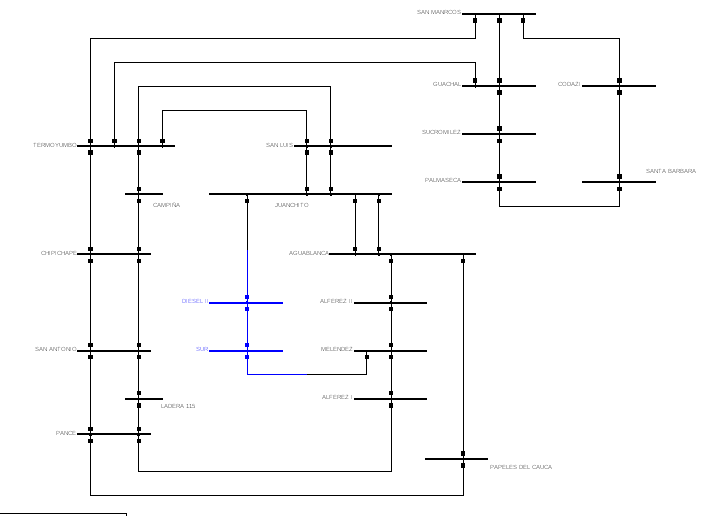
\includegraphics[width=\linewidth]{str}
\end{figure}
\section{SDL: Sistema Distribución Local}
Conjunto de líneas y subestaciones, con sus equipos asociados, que operan en los Niveles de Tensión 4, 3, 2 y 1 que no pertenecen las \ac{STR} y son usadas para el sistema de distribución local.

\begin{center}

  \begin{tcolorbox}[ title=SDL:Nivel de tensión 4]
    {57.5 kV $\leq$ V < 220 kV }
\end{tcolorbox}

  \begin{tcolorbox}[ title=SDL:Nivel de tensión 3]
    {30 kV $\leq$ V < 57.5 kV }
\end{tcolorbox}
\begin{tcolorbox}[ title=SDL:Nivel de tensión 2]
  { 1 kV $\leq$ V < 30 kV }
  \end{tcolorbox}
\begin{tcolorbox}[ title=SDL:Nivel de tensión 1]
  { V < 1 kV }
  \end{tcolorbox}
\end{center}

Por otra parte de acuerdo  al \ac{RETIE} \cite{RETIE2013} en el articulo 12, las instalaciones se pueden clasificar de acuerdo al nivel de tensión en función de su riesgo:\\\\
\begin{itemize}
\item Extra alta tensión > 230 kV
\item  230 kV  $\leqslant$ Alta tensión  > 57.5 kV .
\item 57.5 kV  $\leqslant$ Media tensión  > 1 kV .
\item Baja tensión < 1kV.
\end{itemize}

\section{ACTIVOS DE CONEXIÓN}

Los activos de conexión y activos de uso son descritos en  la resolución \cite{CREG0972008}. 

\begin{figure}[H]
  \centering
  \caption{Activos de conexión y activos de uso del \ac{SIN}}
  \label{fig:activosdeuso}
  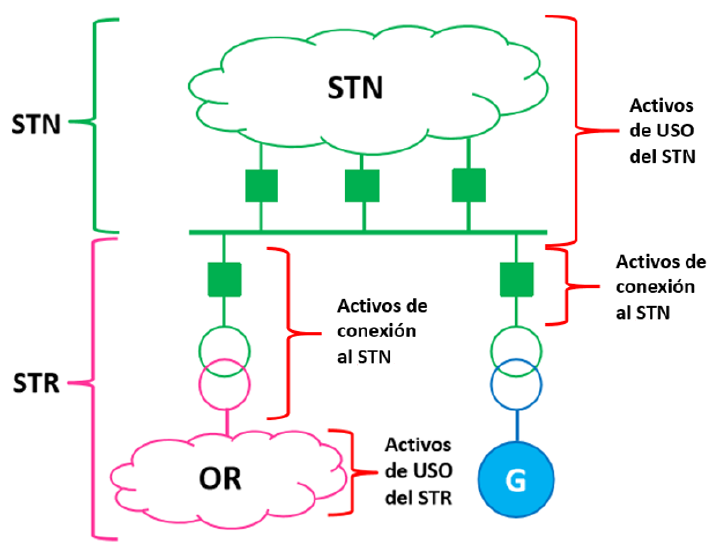
\includegraphics[width=\linewidth]{activos_de_conexion}
\end{figure}


\section{AREAS DE DISTRIBUCIÓN}
Conjunto de redes de Transmisión Regional y/o Distribución Local
destinado a la prestación del servicio en zonas urbanas y rurales, que
son operadas por uno o más Operadores de Red y que se conforman
teniendo en cuenta la cercanía geográfica de los mercados atendidos y
el principio de neutralidad establecido en la ley, y se establece que
debe existir un Cargo Único por Nivel de Tensión por cada ADD \cite{CREG1332013}.\\\\
\begin{itemize}
\item Oriente
\item  Occidente
\item  Sur 
                            \item  Centro
\end{itemize}

\section{AGENTES DEL SECTOR}
Los agentes del mercado son los encargados de producir, llevar y vender la energía al usuario final. Se clasifican en generadores, transmisores, distribuidores, comercializadores y administradores, según el rol que desempeñan.

\paragraph{Generadores}

Son los encargados de producir la energía por medio de centrales hidráulicas, térmicas y eólicas.
\paragraph{Transmisores}

Son los encargados de transportar largas distancias la energía desde las centrales eléctricas hasta las subestaciones de transformación a través de redes que operan a tensiones iguales o superiores a 220 kV.
\paragraph{Distribuidores}

Son los encargados de llevar la energía hasta el consumidor final a través de redes que operan a tensiones inferiores a 220 kV.
\paragraph{Comercializadores}

Son los encargados de la compra de energía eléctrica en el mercado mayorista y su venta a usuarios finales.

  
\chapter{PLANEACIÓN DE LA EXPANSIÓN DEL STN, STR Y SDL }

%La entidad encargada de realizar la planeación del \textbf{STN} es la \ac{UPME}.\\\\
La planeación de la operación se basa en tres ejes de acuerdo a la ley 143 \cite{LEY143} en el articulo 33, que son \textbf{confiable}, \textbf{segura} y con \textbf{calidad del servicio}.\\

\chapter{OPERACIÓN DEL SIN}

La operación del \ac{SIN}, comprende las siguientes componentes y esta a cargo del \ac{CND}:

\begin{enumerate}
\item Planeamiento Operativo
\item Despacho Económico
\item la coordinación
\item La supervición y control
\end{enumerate}

\section{PLANEAMIENTO OPERATIVO}

Se hace de forma integrada, garantizando seguridad, confiabilidad y
calidad de servicio \cite{CREG0251995}. Se descompone funcionalmente
como muestra la figura \ref{fig:planeamineto-operativo}\\\\

\begin{figure}[H]
  \centering
  \caption{Descomposición funcional y temporal del Planeamiento
    Operativo}
  \label{fig:planeamineto-operativo}
  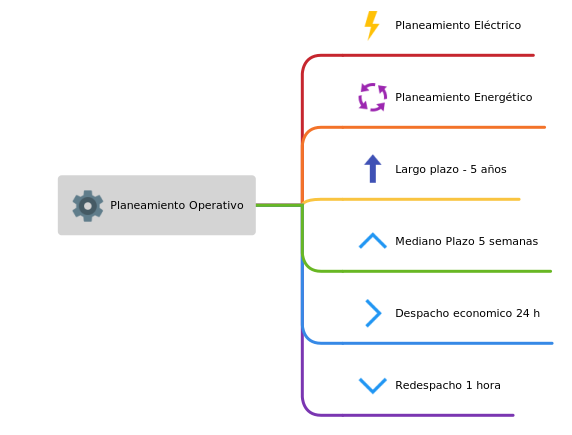
\includegraphics[width=1\linewidth]{planeamineto-operativo}
\end{figure}

\subsection{PLANEAMIENTO ENERGÉTICO}

Consiste en la planeación de la operación de los recurso energéticos,
hidráulicas y térmicos para la producción de energía eléctrica
\cite{CREG0251995}.

\section{DESPACHO ECONÓMICO}
Proceso mediante el cual se obtiene para un período de 24 horas, el programa horario de generación de los recursos del SIN despachados centralmente. Este despacho se efectúa con el criterio de minimizar el costo de atender la demanda.

En el numeral 1.3 del Código de Operación que hace parte del Código de Redes, adoptado mediante la Resolución CREG 025 de 1995, se definen las plantas despachadas centralmente de la siguiente forma:

\paragraph{Plantas Centralmente Despachadas}:

 Son todas las plantas de generación con capacidad efectiva mayor que 20 MW y todas aquellas menores o iguales a 20 MW que quieran participar en el Despacho Económico. 


\chapter{CONTROL DE TENSIÓN}

En estado estacionario las tensiones en las barras de 115 kV,
  110 kV y 220 kV, 230 kV no deben ser inferiores al 90\% ni
  superiores al 110\% del valor nominal. Para la red de 500 kV el
  voltaje mínimo permitido es del 90\% y el máximo es del 105\% del
  valor nominal \cite{CREG0251995}.\\\\

Para realizar el aumento de tensión se siguen con los pasos desarrollados en la figura:

\begin{figure}[H]
  \centering
  \caption{Aumento de tensión}
  \label{fig:aumentotension}
  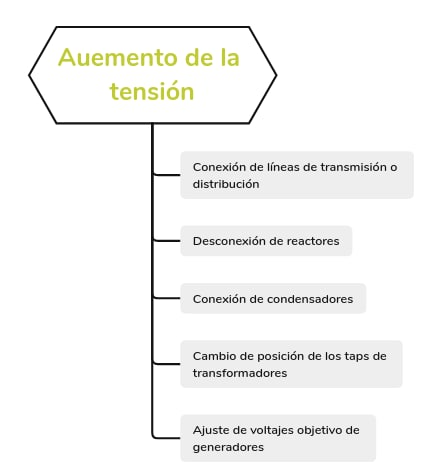
\includegraphics[width=0.8\linewidth]{aumentartension}
\end{figure}

Para reducir la tensión se procederá con los siguientes procesos:

\begin{figure}[H]
  \centering
  \caption{Reducción de  tensión}
  \label{fig:reducciontension}
  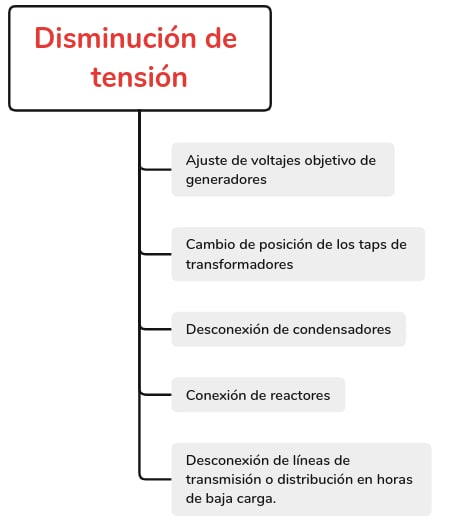
\includegraphics[width=0.8\linewidth]{reducirtension}
\end{figure}

  


\chapter{CONTROL DE FRECUENCIA}

De acuerdo al la resolución CREG 061 de 1996 se establece el esquema de desconexión automática de carga debe cumplir los siguientes criterios \cite{CREG0611996}:\\\\

\begin{itemize}
\item El disparo de la unidad de mayor capacidad del sistema no deberá activar la primera etapa de
desconexión
\item En ningún momento la frecuencia podrá ser inferior a 57.5 Hz
\item En contingencias se debe minimizar el tiempo que la frecuencia permanezca por debajo de 58.5 Hz
\item Después de 10 segundos de ocurrido un evento, la frecuencia del sistema deberá estar por encima
del umbral de la primera etapa del EDAC
\item Se deberá optimizar la cantidad de carga a desconectar en eventos, evitando al máximo la sobre
frecuencia, es decir, frecuencias superiores a 60 Hz después de ocurrido un evento
\end{itemize}

Para el año 2017 se aprobó el Esquema de Deslastre de Automático de
Carga EDAC por baja frecuencia que cubra un 40\% el total de la
demanda, distribuido en 8 etapas con desconexiones de carga del 5\%
\textbf{(Acuerdo 964} del 4 de mayo de 2017 ), El cual es ilustrado en
las figuras \ref{fig:edac}, \ref{fig:edac1} y \ref{fig:edac2}.

\begin{figure}[H]
  \centering
  \caption{Esquema EDAC}
  \label{fig:edac}
  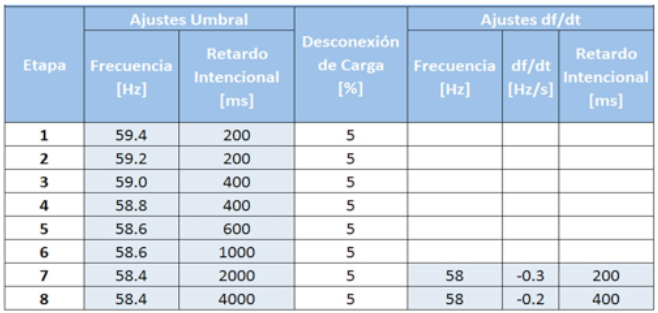
\includegraphics[width=0.8\linewidth]{esquema_edac}
\end{figure}

\begin{figure}[H]
  \centering
  \caption{Representación gráfica del esquema EDAC}
  \label{fig:edac1}
  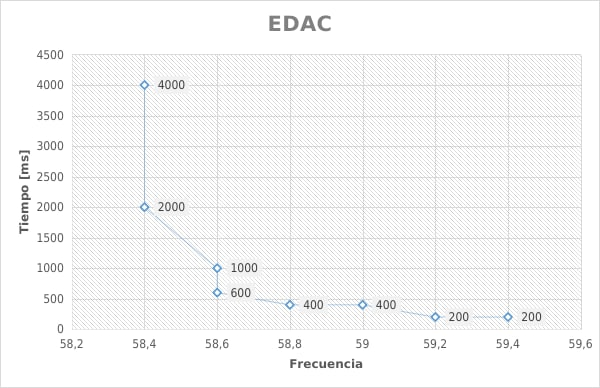
\includegraphics[width=0.8\linewidth]{EDAC1}
\end{figure}

\begin{figure}[H]
  \centering
  \caption{Representación gráfica del esquema EDAC}
  \label{fig:edac2}
  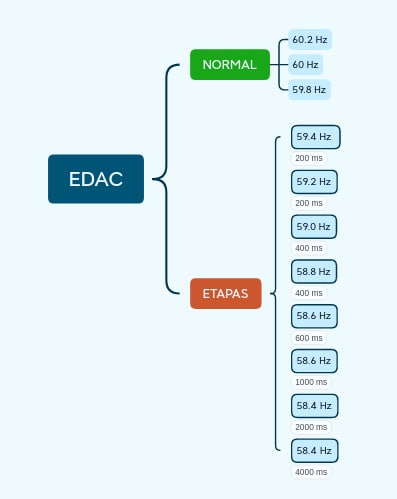
\includegraphics[width=0.8\linewidth]{EDAC}
\end{figure}


\

\chapter{PRONOSTICO DE LA DEMANDA}

Es un valor \textit{estimado} de la energía demandada en un mercado de
comercialización y su desagregación por centro de consumo. Este
pronóstico se propone por el CND antes del día míercoles y se corrige
por el OR hasta el viernes para si constituir el pronóstico oficial
del OR para su mercado de comercialización de la semana siguente ( de
lunes a Domingo). Durante la semana se pueden realizar ajustes antes
de las 7:30 a.m.\\\\
Para la estimación de la demand real el CND utiliza la siguiente
ecuación en un mercado de comencialización :\\\\
\[D_{real} = importacion + generacion - exportacion \]




\chapter{ESTABILIDAD}
 En el análisis de estado estacionario se consideran solo
  contingencias sencillas en las líneas de transmisión y en los bancos
  de transformadores 230/115 kV o 220/110 kV.\\\\
	
	
 Las corrientes e impedancias vistas por los relés vecinos, deben
  ser tales que no ocasionen la salida de elementos adicionales, lo
  cual originaría una serie de eventos en cascada.  En las barras
  principales del sistema de transmisión la tensión transitoria no
  debe estar por debajo de 0.8(p.u.) durante más de 500 mseg.\\\\
	
 Al evaluar la estabilidad del sistema de transmisión ante
  pequeñas perturbaciones, se debe chequear que los valores propios
  tengan componente de amortiguación. Si no hay amortiguación se deben
  ajustar apropiadamente los sistemas de control de las unidades de
  los equipos del SIN y como último recurso, limitar las
  transferencias por el sistema de transmisión.\\\\


  \chapter{EVENTOS}

  \section{MARCO REGULATORIO}

\begin{center}
\begin{tcolorbox}
La Ley 143 de 1994, en sus Artículos 34 y 38, establece las responsabilidades del Centro Nacional de Despacho (CND) en la coordinación, supervisión, control y análisis de la operación de los recursos del SIN, así como la obligación de las empresas generadoras, distribuidoras y operadoras de redes de suministro de información oportuna y fiel al CND y los CRD's.
\end{tcolorbox}
\end{center}

  La \textbf{Resolución CREG 080 de 1999} define las responsabilidades del CND y los agentes del SIN en la realización de estudios sobre fallas y emergencias. La \textbf{Resolución CREG 083 de 1999} detalla la información obligatoria que los agentes deben adquirir y suministrar al CND, incluyendo registros cronológicos de eventos con alta resolución temporal y libre acceso a esta información.\\\\ 
  
  Las Resoluciones \textbf{CREG 093} ( para el \ac{STN}) y \textbf{094 de 2012} ( para el STR) requieren informes detallados para eventos no programados que superen un cierto umbral de \ac{PENS}.\\\\

\begin{figure}[H]
   \centering
   \caption{Metodología del calculo del pronostico de la energía no
     suministrada}
   \label{fig:ens}
   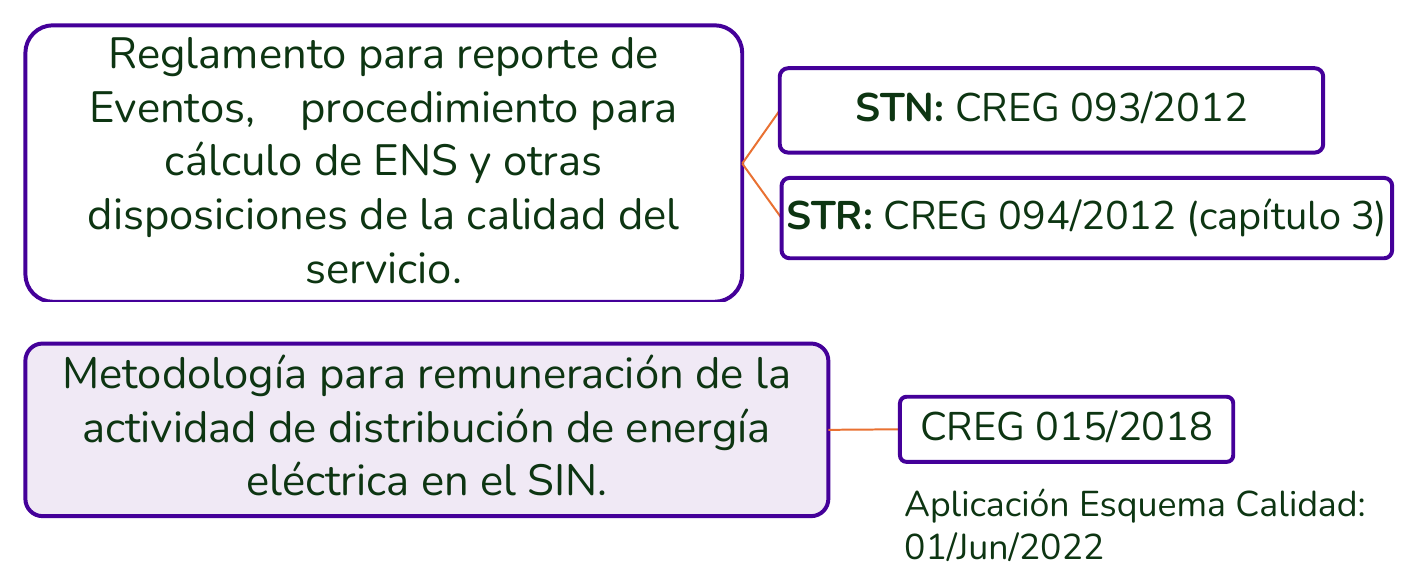
\includegraphics[width=\linewidth]{calculo_ens.png}
 \end{figure}

 
\subsection*{Ejemplo Numérico Hipotético del Pronóstico Nuevo de Demanda ($PRN_{j,h}$)}

El Pronóstico Nuevo de Demanda ($PRN_{j,h}$) se utiliza en el procedimiento de cálculo de la Energía No Suministrada (ENS) definido en el Capítulo III de la Resolución 94 de 2012 CREG [1, 2].

La fórmula utilizada es:
\begin{equation}
	PRN_{j,h} = PR_{j,h} \cdot \left( \frac{DE_{j,a}}{PR_{j,a}} \right)
\end{equation}
Donde:
\begin{itemize}
	\item $PRN_{j,h}$: Pronóstico Nuevo de Demanda para el periodo horario $h$ [3].
	\item $PR_{j,h}$: Pronóstico de demanda utilizado en el Despacho Económico para el periodo horario $h$ [3].
	\item $DE_{j,a}$: Demanda Entregada en el periodo horario $a$ [3].
	\item $PR_{j,a}$: Pronóstico de demanda utilizado en el Despacho Económico para el periodo horario $a$ [3].
	\item $h$: Periodo horario en el que se presenta el Evento (o el siguiente, si subsiste) [3].
	\item $a$: Último periodo horario completo, anterior al Evento, sin efecto en la demanda atendida causado por otros Eventos en el STR [3].
\end{itemize}

\subsubsection*{Valores Hipotéticos para el Mercado $j$}
Se asumen los siguientes valores (los cuales no provienen de las fuentes regulatorias):
\begin{center}
	\begin{tabular}{|l|l|c|}
		\hline
		\textbf{Variable} & \textbf{Definición} & \textbf{Valor Hipotético (MW)} \\
		\hline
		$PR_{j,h}$ & Pronóstico de Demanda (Hora $h$) & $650$ \\
		$PR_{j,a}$ & Pronóstico de Demanda (Hora $a$) & $600$ \\
		$DE_{j,a}$ & Demanda Entregada (Hora $a$) & $612$ \\
		\hline
	\end{tabular}
\end{center}

\subsection*{Cálculo}

\begin{enumerate}
	\item \textbf{Cálculo del Factor de Ajuste ($\frac{DE_{j,a}}{PR_{j,a}}$)}
	Este factor ajusta el pronóstico horario $h$ basándose en la precisión del pronóstico en el periodo $a$.
	\begin{equation*}
		\text{Factor de Ajuste} = \frac{612 \, \text{MW}}{600 \, \text{MW}} = 1.02
	\end{equation*}
	
	\item \textbf{Cálculo del Pronóstico Nuevo de Demanda ($PRN_{j,h}$)}
	Se aplica el factor de ajuste al Pronóstico de Demanda original para el periodo $h$ ($PR_{j,h}$):
	\begin{align*}
		PRN_{j,h} &= PR_{j,h} \cdot (\text{Factor de Ajuste}) \\
		PRN_{j,h} &= 650 \, \text{MW} \cdot 1.02 \\
		PRN_{j,h} &= \mathbf{663 \, \text{MW}}
	\end{align*}
\end{enumerate}

\vspace{0.5cm}

El valor de $\mathbf{PRN_{j,h}} = 663 \, \mathbf{MW}$ es el \textit{Pronóstico Nuevo de Demanda} que se utilizará para calcular la Energía No Suministrada ($ENS_{MHj,h}$) para el periodo horario $h$.\\\\




El Acuerdo 1617 introduce actualizaciones basadas en las Resoluciones \textbf{CREG 015 de 2018}, \textbf{036 de 2019} y \textbf{101023 de 2022}, incluyendo la responsabilidad de reporte de información por parte de los Operadores de Red (OR), los plazos para reportar el valor de la Energía No Suministrada (ENS) al LAC, y la inclusión de eventos no programados en los Sistemas de Almacenamiento de Energía Eléctrica con Baterías (SAEB). Los Anexos 1 y 2 detallan el procedimiento y los formatos específicos para la elaboración de estos informes.

\section{REPORTE DE EVENTOS Y ENERGÍA NO SUMINISTRADA}

Cuando ocurre un evento programado (manenimiento ) o no programado (falla)  tiene como consecuencia la  indisponibilidad total o parcial  de un activo \cite{CREG0942012}. Cuando esta indisponibilidad causa un ausencia de tensión  en parte de la red y el \ac{PENS} supera el 2\% ,  el \ac{CND} envía a la Superintendencia de Servicios Públicos Domiciliarios, SSPD, un informe donde se haga el análisis detallado del Evento ocurrido y contenga como mínimo lo siguiente \cite{CREG0152018}.


 \begin{itemize}
 \item Número y descripción de los eventos.
 \item Activos causantes de los eventos.
 \item Valores y memoria de cálculo de las variables para cálculo de ENS.
 \item Para los MC afectados, curva de potencia activa del periodo horario del evento.
 \item De los 12 periodos anteriores y de los 12 siguientes a la ocurrencia del mismo.
 \item Informe final del evento previsto en los acuerdos del CNO.
 \end{itemize}


 ”… Y en su articulo 24, adiciona el siguiente párrafo al final del numeral 5.1.14.2 Compensaciones por dejar no operativos otros activos o por energía no suministrada: “Cuando el valor del PENS supere el 2\%, los OR tendrán un plazo de dos días, contados a partir de la publicación por parte del CND del informe de ENS, para reportar el valor de la ENS al LAC
 
\begin{figure}[H]
 816   \centering
 817   \caption{Estructura informe de eventos acuerdo CNO 1617}
 819   \label{fig:estructurainforme}
 820   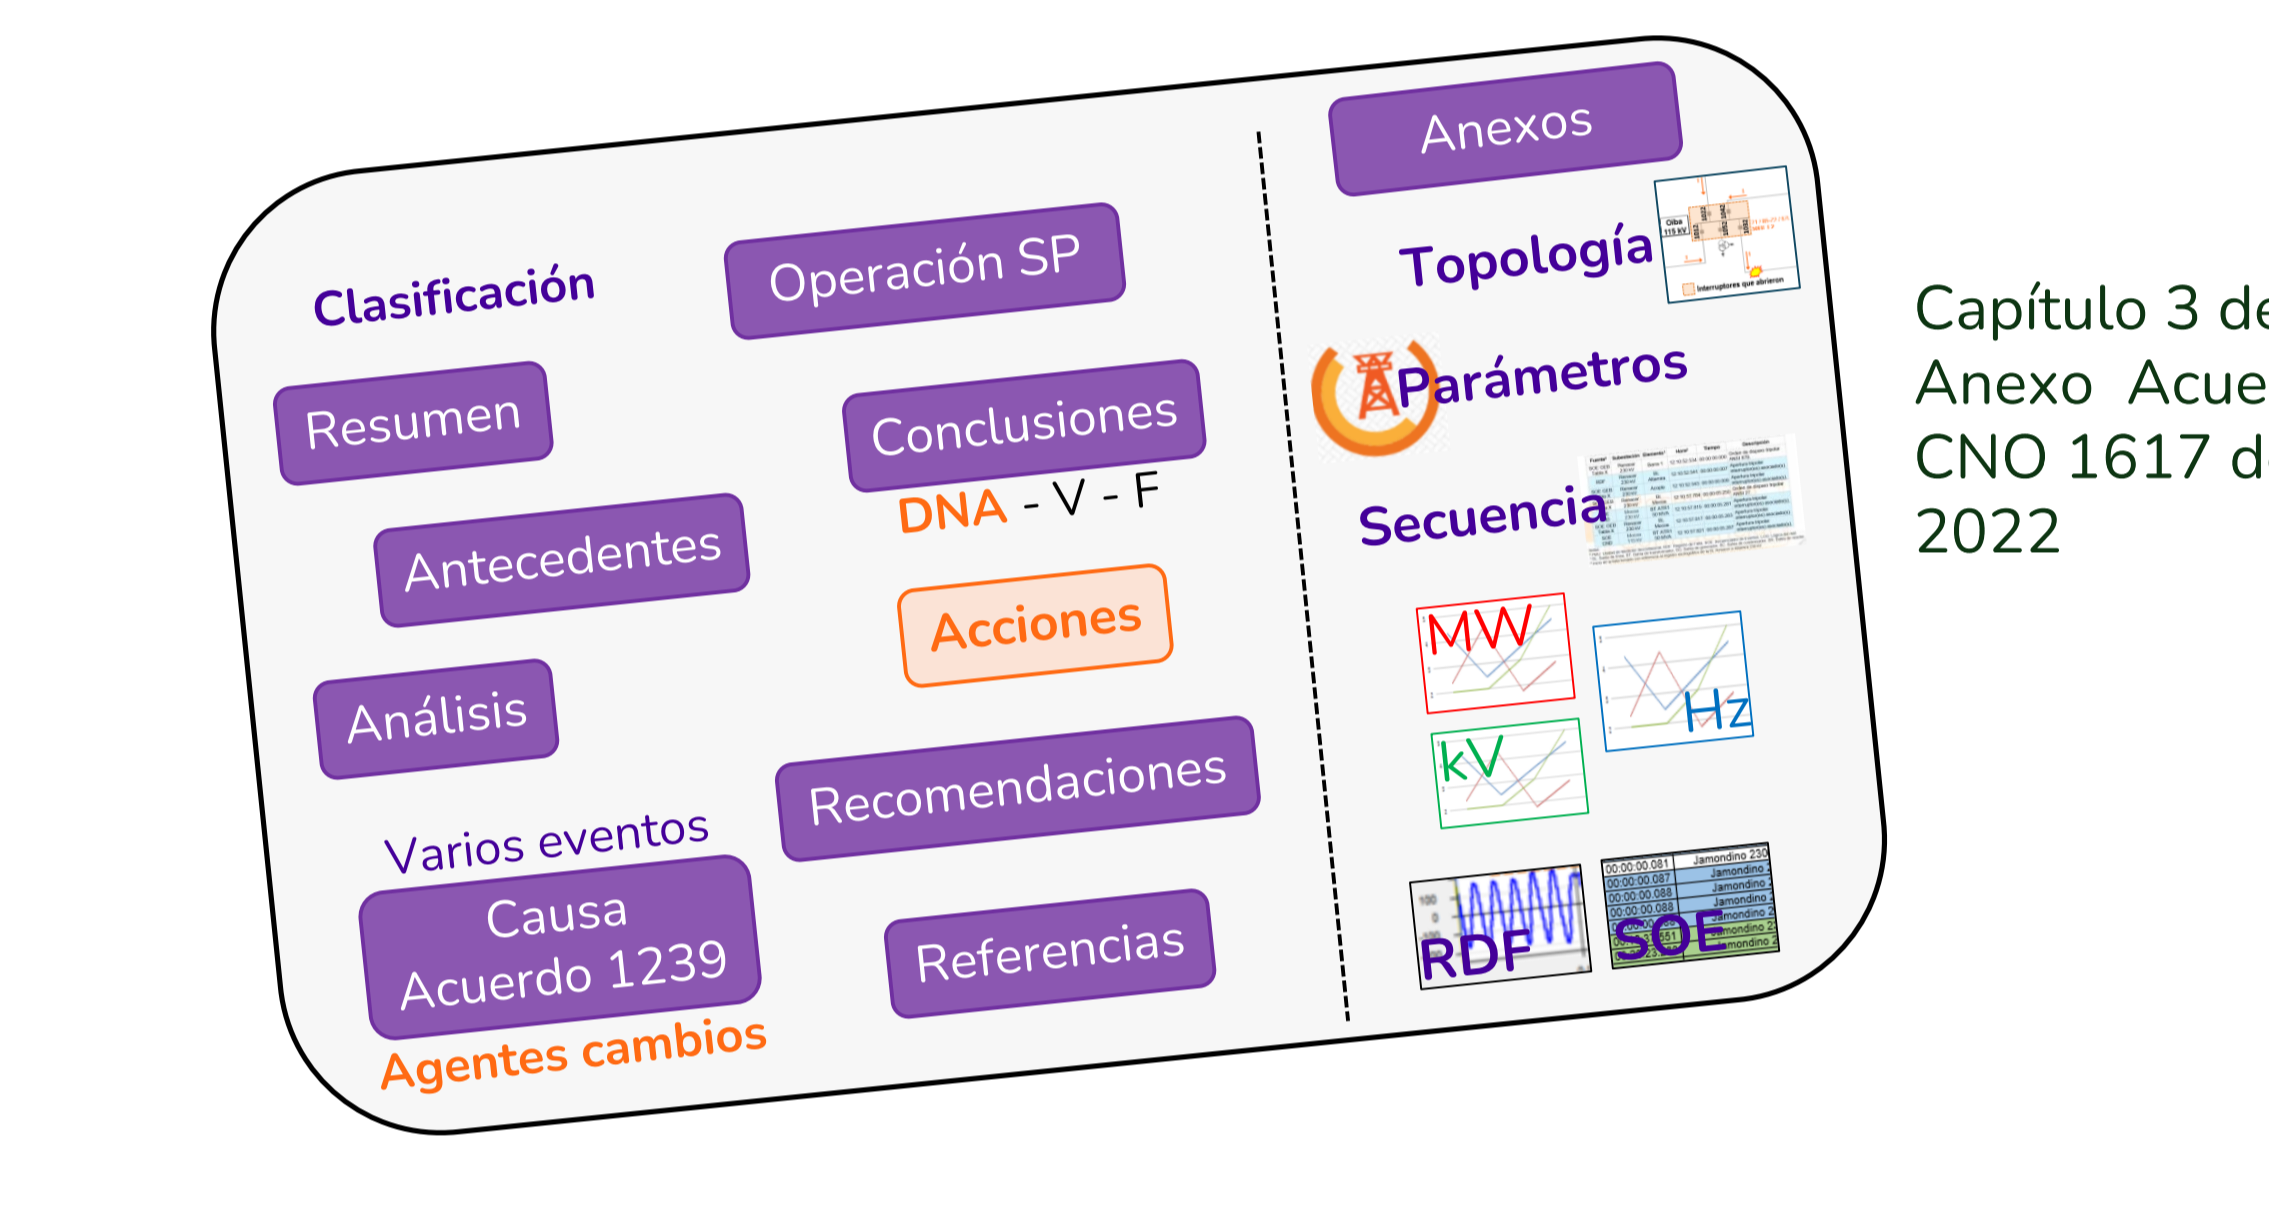
\includegraphics[width=\linewidth]{estructura_informe_eventos1617}
 821 \end{figure}


La energía con la que se calcula la \ac{ENS} es la reportada por los distintos comercializadores del mercado de comercialización.

  \section{ANÁLISIS DE EVENTOS}



\begin{figure}[H]
  \centering
  \caption{insumos para el análisis de eventos}
  \label{fig:insumoseventos}
  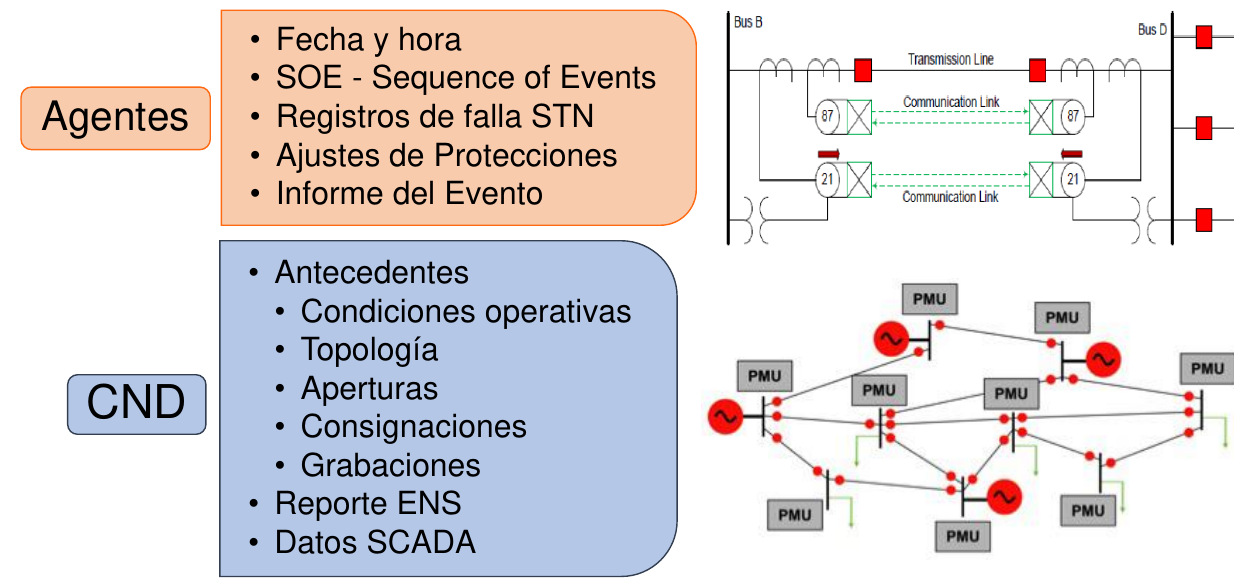
\includegraphics[width=0.8\linewidth]{insumos_eventos}
\end{figure}

\subsubsection{Responsables de los análisis y elaboración de informes}

\begin{itemize}
  
\item CND: Eventos en Activos de Uso del STN, Activos de Conexión al STN, Interconexiones Internacionales de nivel IV o superior, y otros que ameriten análisis.
    
  \item Transportadores de energía eléctrica en el \ac{STN} y/o Servicio de Conexión al \ac{STN}: Eventos en sus activos del \ac{STN}, incluyendo Interconexiones Internacionales con tensión igual o superior a 220 kV y Activos de Conexión al \ac{STN}.
  
  \item Operadores de Red (OR's): Eventos en los activos bajo su supervisión. Los OR son los responsables de la recolección y el reporte de la información de eventos y la requerida para la aplicación de las disposiciones de calidad del servicio. Cuando el OR no opere los activos directamente, la información será reportada por quien los opera, y en el respectivo contrato de operación podrán precisarse los mecanismos para que el OR conozca la información reportada al CND. En todo caso, el responsable de la calidad y la oportunidad de la información reportada, a través del sistema dispuesto por el CND para este fin, es el agente a quien se le están remunerando los activos.
    
  \item Generadores: Deben suministrar información de plantas de generación si el \ac{CND} la requiere para sus análisis.

\end{itemize}



\subsection{Eventos a los que aplica el procedimiento de análisis}

\begin{itemize}
\item\textit{ Eventos no programados} que requieran análisis según Resoluciones CREG 093/2012, 094/2012 (Capítulo 3) y 015/2018.
\item Eventos en conexión internacional que originen \textit{separación de ambos sistemas eléctricos}.
    
\item Eventos que ocasionen la desconexión de \textit{2 o más} activos del STN (STN > N - 1).
    
\item Eventos en nivel de tensión IV o superior que generen la \textit{desconexión de todos los elementos} asociados a una barra o sección de barra.
    
\item Eventos que apliquen para análisis por \ac{SAEB}, cuando se cumplan los requerimientos regulatorios (\textbf{Resolución CREG 101023 de 2022}).
    
\item Eventos en el SIN que el CND considere que requieren análisis.
    
\item Eventos para los cuales los agentes soliciten análisis, previo acuerdo con el CND.

\end{itemize}
    
\subsection{Información a reportar por parte de los agentes}

 Identificación del activo, fecha y hora del evento, \ac{SOE} en formato editable, registros de falla originales (COMTRADE), ajustes de protecciones involucradas (si no están actualizados en la base de datos del CND), y cualquier información adicional pertinente.\\\\
Un informe detallado y completo del evento, siguiendo la estructura establecida en el Anexo 1.

\subsection{Estructura de los informes}

    Informe de Agentes: Resumen general, antecedentes (cuando aplique), análisis, causa (incluyendo activo causante y causas de desconexiones adicionales), operación de sistemas de protección, conclusiones (descripción del evento, operación de protecciones, DNA, ausencia de tensión, actuación EDAC/ESP/ESPS, otros hallazgos), acciones (ejecutadas y por ejecutar), recomendaciones, anexos.\\\\
    Informe del CND: Integra la información de los agentes, e incluye además: excursión de frecuencia en el resumen, recurrencia de inconvenientes en antecedentes, variación de frecuencia y cumplimiento de reglamentación en conclusiones, acciones y recomendaciones adicionales, referencias, y anexos opcionales (topología, secuencia del evento, condiciones operativas, otra información).\\\\
    Informes de Casos Especiales (Anexo 2): Aplicable a eventos específicos (retraso en consignación, disparo de generador, omisión de cierre, apertura manual no programada, SAEB, evento N-1 con PENS > 2\%). Tienen una estructura simplificada y no requieren revisión de agentes a menos que el CND identifique modificaciones necesarias.

\subsection{Plazos definidos para cada etapa del proceso (días hábiles a partir del día cero)}

Los plazos para la presentación del informe pueden agilizarse o prolongarse de acuerdo al los acuerdos con los agentes.

\begin{figure}[H]
  \caption{Plazo acuerdo CNO 1617 de 2022}
  \label{fig:plazo1617}
  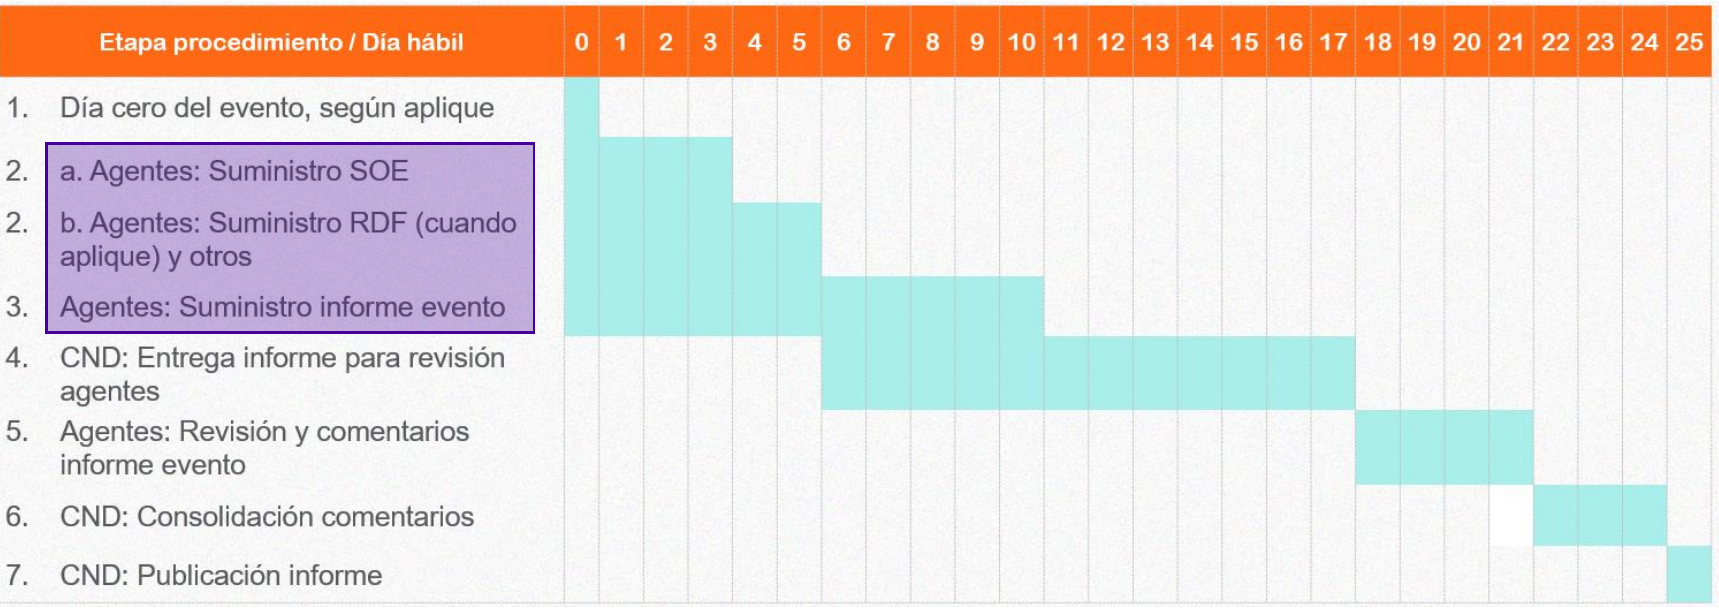
\includegraphics[width=\linewidth]{plazo16172022}
 \end{figure}

Suministro de SOE en el mínimo tiempo posible, RDF en 48-72 horas.\\\\
Reuniones para redefinir plazos, acuerdo con el CND para plazos adicionales de suministro de información con justificación escrita. El CND informará al CNO sobre estas prolongaciones.

\subsection{Seguimiento de Acciones}

    Responsabilidad de los agentes es informar al CND la fecha de ejecución de acciones, número de consignación nacional y soportes técnicos.\\\\
    El CND mantendrá disponible el estado de las acciones, enviará trimestralmente un seguimiento al subcomité de protecciones y lo presentará en comités del CNO.\\\\
    Las acciones solo se podrán reprogramar con un \textit{plan de acción}, fechas específicas y justificación.

\section{Preguntas de Quiz (10 preguntas de respuesta corta)}

\begin{enumerate}
\item ¿Cuál es la fecha de expedición y de entrada en vigencia del Acuerdo CNO 1617, y a qué acuerdo sustituye?
\item Según el Artículo 34 de la Ley 143 de 1994, ¿cuál es una función clave del CND?
\item ¿Qué tipo de información específica es obligatoria para los agentes del \ac{SIN} según la Resolución CREG 083 de 1999 para el análisis de eventos?
\item ¿Qué umbral de \ac{PENS} hace necesario un informe final detallado según las resoluciones CREG 093 y 094 de 2012, y quién es el responsable de publicarlo?
\item ¿Quiénes son los responsables de la recolección y el reporte de la información de eventos y de la calidad del servicio según la Resolución \textbf{CREG 036 de 2019}?
\item ¿Cuál es el objetivo principal del procedimiento establecido en el \textbf{Anexo 1} del Acuerdo 1617?
    Mencione tres tipos de eventos a los que aplica el procedimiento de análisis de eventos del Acuerdo \textbf{CNO 1617}.
  \item Además de la identificación del activo y la fecha/hora, ¿qué otros dos tipos de información técnica mínima deben suministrar los agentes al \ac{CND} para el análisis consolidado de eventos?
  \item ¿Cuál es la diferencia en el "día cero" para eventos relacionados con \ac{ENS}/\ac{PENS} y para otros eventos no programados según los plazos definidos?
  \item ¿Qué deben hacer los agentes si identifican que la información inicialmente reportada sobre el activo causante de un evento difiere del análisis detallado?
  \end{enumerate}
  
  \subsection{Clave de Respuestas del Quiz}

  \begin{itemize}

  \item El Acuerdo CNO 1617 fue expedido el 06 de Octubre de 2022 y entró en vigencia el 06 de Noviembre de 2022. Sustituye al Acuerdo 03/09/2015, Acuerdo 787.
  \item Según el literal b. del Artículo 34 de la Ley 143 de 1994, es función del CND "ejercer la coordinación, supervisión, control y análisis de la operación de los recursos de generación, interconexión y transmisión incluyendo las interconexiones internacionales".
  \item La Resolución CREG 083 de 1999 establece como obligatoria la remisión de: a) Registro sobre la secuencia cronológica de eventos (SOE) y b) Por cada evento, fecha y hora con resolución de un (1) ms, identificación del elemento que cambió de estado y el estado final del dispositivo.
  \item Un informe final detallado es necesario cuando el \textbf{PENS} supere el \textbf{2\%}. El CND es el responsable de elaborar y publicar este informe sobre \ac{ENS}.
  \item Los Operadores de Red (OR) son los responsables de la recolección y el reporte de la información de eventos y la requerida para la aplicación de las disposiciones de calidad del servicio. En todo caso, el responsable de la calidad y oportunidad de la información es el agente a quien se le remuneran los activos.
  \item El objetivo principal es establecer un procedimiento para la elaboración de los informes de análisis de eventos en el Sistema Interconectado Nacional (SIN) por parte del CND y los agentes del SIN.
  \item Tres tipos de eventos a los que aplica son: a) Eventos no programados que requieran análisis según Resoluciones CREG 093/2012, 094/2012 (Capítulo 3) y 015/2018; b) Eventos en conexión internacional que originen separación de ambos sistemas eléctricos; c) Eventos que ocasionen la desconexión de 2 o más activos del STN (STN > N - 1); d) Eventos en nivel de tensión IV o superior, que generen la desconexión de todos los elementos asociados a una barra o sección de barra; e) Eventos que apliquen para análisis por SAEB. (Cualquiera de estas tres son válidas).
  \item Los agentes deben suministrar el SOE (Sequence Of Events) en formato editable y los registros de falla originales (sin editar), en formato COMTRADE o estándar sustituto.
    Para eventos que deban ser analizados según ENS/PENS (numeral 'a'), el día cero (0) es la fecha en la cual el CND publica el cálculo de Energía No Suministrada (ENS). Para los demás criterios (numerales 'c', 'd', 'f', 'g'), el día cero es el día de ocurrencia del evento.
  \item Si el activo que dio origen al evento difiere de la información inicialmente reportada, los agentes son responsables de solicitar al CND las modificaciones de la información correspondiente en dicho reporte de eventos, en caso de que aplique.
    \end{itemize}

\subsection{Preguntas de Formato Ensayo}
\begin{itemize}
\item Compare y contraste las responsabilidades del CND y de los Agentes del SIN en la elaboración y suministro de información para los informes de análisis de eventos, detallando cómo se complementan sus roles según el Acuerdo 1617.
   
\item  Analice la importancia de los plazos establecidos en el Acuerdo 1617 para la eficiencia y la efectividad del proceso de análisis de eventos. Discuta las "Consideraciones para agilizar los plazos" y "Consideraciones para prolongar los plazos", y cómo estas buscan equilibrar la celeridad con la profundidad del análisis.
    
\item Describa la evolución de la regulación del sector eléctrico que ha llevado a la expedición del Acuerdo 1617, haciendo referencia a al menos cuatro resoluciones CREG mencionadas y explicando cómo cada una contribuye al marco regulatorio actual del análisis de eventos.
\item Explique en detalle la estructura requerida para un informe de análisis de eventos elaborado por los agentes del SIN, tal como se describe en el numeral 3.2 del Anexo 1. Incluya los componentes obligatorios y su propósito en la identificación de la causa raíz y las acciones correctivas.
\item Discuta el rol de los "Casos Especiales" en el procedimiento de análisis de eventos, tal como se definen en el numeral 3.4 y el Anexo 2. Explique por qué ciertos eventos se clasifican como especiales y cómo su tratamiento difiere del procedimiento estándar para eventos más complejos.
\end{itemize}
\subsection{Glosario de Términos Clave}

\texttt{\begin{itemize}
  \item Acuerdo CNO 1617: Documento que actualiza el procedimiento para la elaboración de informes de análisis de eventos en el Sistema Interconectado Nacional (SIN).
  \item Activo: Se refiere a cualquier elemento o componente del Sistema Interconectado Nacional, según las definiciones de las Resoluciones CREG 011 de 2009 y CREG 015 de 2018.
  \item Agente Generador: Empresa encargada de la producción de energía eléctrica dentro del SIN.
  \item Agentes del SIN: Las empresas generadoras de electricidad, las distribuidoras y las que operan redes de interconexión y transmisión dentro del Sistema Interconectado Nacional.
  \item CND (Centro Nacional de Despacho): Entidad central en el SIN responsable de la coordinación, supervisión, control y análisis de la operación del sistema, incluyendo la gestión de información de eventos.
  \item CNO (Consejo Nacional de Operación): Órgano que aprueba acuerdos y procedimientos relacionados con la operación del SIN.
  \item COMTRADE: Estándar para el intercambio de datos de registros de falla, utilizado para los registros oscilográficos en el análisis de eventos.
  \item Consignación Nacional: Proceso formal de autorización para retirar activos del SIN de operación por mantenimiento u otras razones programadas.
  \item CRD’s (Centros Regionales de Despacho): Entidades regionales que apoyan al CND en la coordinación y operación del SIN.
  \item CREG (Comisión de Regulación de Energía y Gas): Organismo regulador que emite resoluciones y normativas para el sector eléctrico en Colombia.
  \item Demanda No Atendida (DNA): Cantidad de energía que la demanda requirió pero no pudo ser suministrada debido a una interrupción o limitación del sistema.
  \item Día Cero (0): El punto de inicio para el conteo de plazos en el procedimiento de análisis de eventos, cuya definición varía según la clasificación del evento.
  \item Disturbio: Evento no planeado que produce una condición anormal en el SIN, como una perturbación o un cambio inesperado en el Error de Control de Área (ACE).
  \item EDAC (Esquema de Desconexión Automática de Carga): Mecanismo de control automático que desconecta bloques de carga para preservar la estabilidad del SIN ante perturbaciones significativas.
  \item ENS (Energía No Suministrada): Energía que no pudo ser entregada a los usuarios finales debido a interrupciones o fallas en el sistema, medida en unidades de energía (e.g., MWh).
  \item Evento: Condición anormal o perturbación en el SIN que requiere análisis, según las Resoluciones CREG 093 de 2012 y CREG 015 de 2018.
  \item ESP/ESPS (Esquemas de Protección / Esquemas de Protección Especiales): Conjuntos de protecciones diseñados para operar ante condiciones específicas del sistema, más allá de la protección básica de los equipos.
  \item Falla: Un evento en el SIN que implica un cortocircuito, una interrupción o una condición de operación anormal de un activo.
  \item Interconexiones Internacionales: Conexiones eléctricas que permiten el intercambio de energía entre el SIN de Colombia y sistemas eléctricos de países vecinos.
  \item Interruptor: Dispositivo de conmutación capaz de interrumpir y establecer corrientes en condiciones normales y anormales del circuito.
  \item LAC (Liquidación y Administración de Cuentas): Se refiere al proceso o entidad encargada de la compensación por energía no suministrada o por otros aspectos económicos del mercado eléctrico.
  \item Ley 143 de 1994: Ley Marco Eléctrica de Colombia que establece los principios generales y las regulaciones del sector energético.
  \item Operador de Red (OR): Empresas encargadas de la operación y el mantenimiento de las redes de transmisión regional (STR) y distribución local (SDL).
  \item PENS (Potencia Equivalente No Suministrada): Una medida de la potencia no entregada a los usuarios, utilizada para clasificar la severidad de los eventos y determinar la necesidad de informes detallados.
  \item Protecciones: Conjunto de dispositivos y sistemas diseñados para detectar fallas o condiciones anormales en el sistema eléctrico y operar equipos (como interruptores) para aislar la falla y proteger la integridad del sistema y los activos.
  \item Registros Oscilográficos: Grabaciones de alta velocidad de las magnitudes eléctricas (corrientes, tensiones) durante un evento, cruciales para el análisis de fallas.
  \item SAEB (Sistemas de Almacenamiento de Energía Eléctrica con Baterías): Tecnologías de almacenamiento de energía que utilizan baterías para gestionar el suministro y la demanda en el SIN.
  \item Seccionador: Dispositivo de conmutación utilizado para aislar eléctricamente una parte del circuito para mantenimiento o seguridad, no diseñado para interrumpir corrientes de falla.
  \item SEP (Sistema Eléctrico de Potencia): Conjunto de elementos interconectados (generación, transmisión, distribución y consumo) que conforman el sistema eléctrico.
  \item SIN (Sistema Interconectado Nacional): La red eléctrica principal de Colombia que conecta las diferentes regiones y fuentes de generación con los centros de consumo.
  \item SOE (Sequence Of Events): Un registro cronológico y detallado de la operación de equipos y protecciones durante un evento, crucial para reconstruir la secuencia de los hechos.
  \item SSPD (Superintendencia de Servicios Públicos Domiciliarios): Organismo que supervisa y controla la prestación de los servicios públicos, incluyendo la energía eléctrica.
  \item STN (Sistema de Transmisión Nacional): La parte de la red de transmisión de energía eléctrica que opera a las tensiones más altas (iguales o superiores a 220 kV), gestionada por los transportadores.
  \item STR (Sistema de Transmisión Regional): La parte de la red de transmisión de energía eléctrica que opera a tensiones intermedias (menores de 220 kV y no parte del SDL), gestionada por los Operadores de Red (OR).
  \item Subcomité de Protecciones: Un comité técnico dentro del CNO que se encarga de analizar y dar concepto favorable a las actualizaciones relacionadas con los sistemas de protección.
  \end{itemize}}


  \section{DEMANDA NO ATENDIDA}

  Es un valor \textit{estimado} de la energía no entregada a la carga
  debido a eventos programados o no programados. Para ello se emplean
  los eventos diarios reportados en ENERGIS.\\\\

  \section{ENERGÍA NO SUMINISTRADA}

  La energía no suministrada es la dejada de entregar a partir de la
  ocurrencia de un evento en el \ac{STR} \cite{CREG0152018}. Esta se
  puede calcular de acuerdo a la siguiente expresión: \cite{CREG0942012}\\\\

  \[ ENSMH_{j,h} = PRN_{j,h} - DE_{j,h} \]

  \begin{tabular}{p{0.2\linewidth} p{0.7\linewidth}}
    Donde :\\\\& \\
    $ENSMH_{j,h}$& Es la energía no suministrada en  un mercado de comercialización a una hora dada \\
    $PRN_{j,h}$ & Es el pronóstico nuevo de la demanda\\
    $DE_{j,h}$ & Es la demanda de electricidad \\
  \end{tabular}\\


    
  \section*{Metodología y Fórmulas}
  
  El CND estima la ENS ($ENSMH_{j,h}$) para cada periodo horario ($h$) y mercado afectado ($j$) como la diferencia entre el Pronóstico Nuevo de Demanda ($PRN_{j,h}$) y la Demanda Entregada ($DE_{j,h}$) [4].
  
  \begin{enumerate}
  	\item \textbf{Energía No Suministrada Horaria ($ENSMH_{j,h}$)}
  	\begin{equation}
  		ENSMH_{j,h} = PRN_{j,h} - DE_{j,h} \quad \text{[4]}
  	\end{equation}
  	
  	\item \textbf{Porcentaje de Energía No Suministrada ($PENS_{j,h}$)}
  	\begin{equation}
  		PENS_{j,h} = \frac{ENSMH_{j,h}}{PRN_{j,h}} \quad \text{[4]}
  	\end{equation}
  	
  	\item \textbf{Condición del Umbral}
  	Si $\mathbf{PENS_{j,h} \le 2\%}$, entonces $\mathbf{ENSMH_{j,h} = 0}$ [4].
  	
  	\item \textbf{ENS del Mercado ($ENSM_j$)}
  	Si $PENS_{j,h}$ supera el 2\%, la $ENSM_j$ es el valor máximo entre la $ENSMH_{j,h}$ del periodo del Evento y la del periodo siguiente (si subsiste el Evento) [4].
  	
  	\item \textbf{ENS Causal Total ($ENS_q$)}
  	Es la sumatoria de las energías no suministradas en cada mercado de comercialización afectado ($NM$) [5]:
  	\begin{equation}
  		ENS_q = \sum_{j=1}^{NM} ENSM_j \quad \text{[5]}
  	\end{equation}
  \end{enumerate}
  
  \section*{Valores Hipotéticos para el Ejemplo}
  
  Asumamos un Evento no programado en el Mercado de Comercialización $j$ durante el periodo horario $h$:
  
  \begin{center}
  	\begin{tabular}{|l|l|c|}
  		\hline
  		\textbf{Variable} & \textbf{Definición} & \textbf{Valor Hipotético (MW)} \\
  		\hline
  		$PRN_{j,h}$ & Pronóstico Nuevo de Demanda (Num. 3.3) & $663$ \\
  		$DE_{j,h}$ & Demanda Entregada en el periodo $h$ & $500$ \\
  		$NM$ & Número de Mercados Afectados & $1$ \\
  		\hline
  	\end{tabular}
  \end{center}
  
  \section*{Cálculo Detallado}
  
  \subsection*{Paso 1: Cálculo de la $ENSMH_{j,h}$ (Energía No Suministrada Horaria)}
  
  \begin{align*}
  	ENSMH_{j,h} &= PRN_{j,h} - DE_{j,h} \quad \text{[4]} \\
  	ENSMH_{j,h} &= 663 \, \text{MW} - 500 \, \text{MW} \\
  	ENSMH_{j,h} &= \mathbf{163 \, \text{MW}}
  \end{align*}
  
  \subsection*{Paso 2: Cálculo del $PENS_{j,h}$ (Porcentaje de Energía No Suministrada)}
  
  \begin{align*}
  	PENS_{j,h} &= \frac{ENSMH_{j,h}}{PRN_{j,h}} \quad \text{[4]} \\
  	PENS_{j,h} &= \frac{163 \, \text{MW}}{663 \, \text{MW}} \\
  	PENS_{j,h} &\approx 0.2458 \quad (\text{o } 24.58\%)
  \end{align*}
  
  \subsection*{Paso 3: Determinación de la ENS del Mercado ($ENSM_j$)}
  
  Se verifica la condición del umbral [4]:
  \begin{itemize}
  	\item $PENS_{j,h} \approx 24.58\%$.
  	\item Como $24.58\% > 2\%$, el $ENSMH_{j,h}$ es válido y no se iguala a cero [4].
  \end{itemize}
  
  Asumiendo que este valor es el máximo $ENSMH_{j,h}$ encontrado en el periodo horario del Evento ($h=1e$) y el siguiente ($h=2e$), la ENS para el Mercado $j$ es:
  \begin{equation*}
  	ENSM_j = 163 \, \text{MW} \quad \text{[4]}
  \end{equation*}
  
  \subsection*{Paso 4: Cálculo de la ENS Causal Total ($ENS_q$)}
  
  Dado que solo se afectó un mercado ($NM=1$):
  \begin{align*}
  	ENS_q &= \sum_{j=1}^{NM} ENSM_j \quad \text{[5]} \\
  	ENS_q &= ENSM_j \\
  	ENS_q &= \mathbf{163 \, \text{MW}}
  \end{align*}
  
  \section*{Resultado}
  
  La Energía No Suministrada ($ENS_q$) causada por el Evento es de $\mathbf{163 \, \text{MW}}$ [5]. Este valor se utiliza en las fórmulas del numeral 11.1.8.2 del anexo general de la Resolución CREG 097 de 2008 para calcular las compensaciones [5]. Adicionalmente, el $PENS_q$ toma el valor del mayor $PENS_{j,h}$ encontrado, que en este caso es 24.58\% [5]. Si este $PENS_q$ supera el 2\%, el CND debe enviar un informe a la SSPD.\\\\
  


  
\hspace{1cm}
  Los datos para el calculo de estos valores son almacenados en la
  base de datos del CND por un tiempo máximo de cinco años en el
  aplicativo HEROPE. Es resposabilidad del OR reportar esta
  información\\\\
  
\chapter{CARGABILIDAD}
\section{CARGABILIDAD DE CIRCUITOS}
 La \textit{máxima transferencia por las líneas} se considera
  como el mínimo valor entre el límite térmico de los conductores,
  máxima capacidad de los transformadores de corriente, el límite de
  transmisión por regulación de voltaje y el límite por estabilidad
  transitoria y dinámica \cite{CREG0251995}.\\\\

  La operación del sistema dentro de los límites de carga
  determinados , exceptuando la sobrecarga de
  transformadores, se consideran como operación normal. Fuera de ellos
  el sistema se considera que está en estado de alerta o de
  emergencia.\\\\
  
Para los circuitos se tendrá como criterio de carga máxima, la
permitida por el conductor en caso de realimentaciones. En condiciones
óptimas  no se debe superar el 70 \% de la capacidad térmica del
conductor \cite{MANOPEMCALI}. En la figura \ref{fig:capacidad_conductores_emcali} se
muestra la capacidad de los conductores empleados en EMCALI.

\begin{figure}[H]
  \centering
  \caption{Capacidad de conductores EMCALI}
  \label{fig:capacidad_conductores_emcali}
  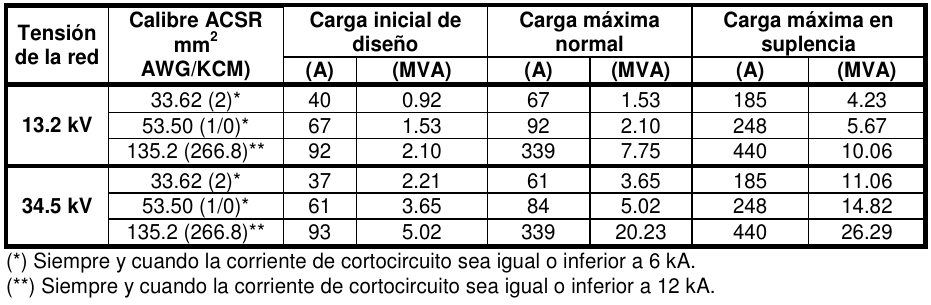
\includegraphics[width=\linewidth]{aereos_emcali}
\end{figure}

\begin{figure}[H]
  \centering
  
  \caption{capacidad de corriente de los conductores}
  \label{fig:ampacidad}
  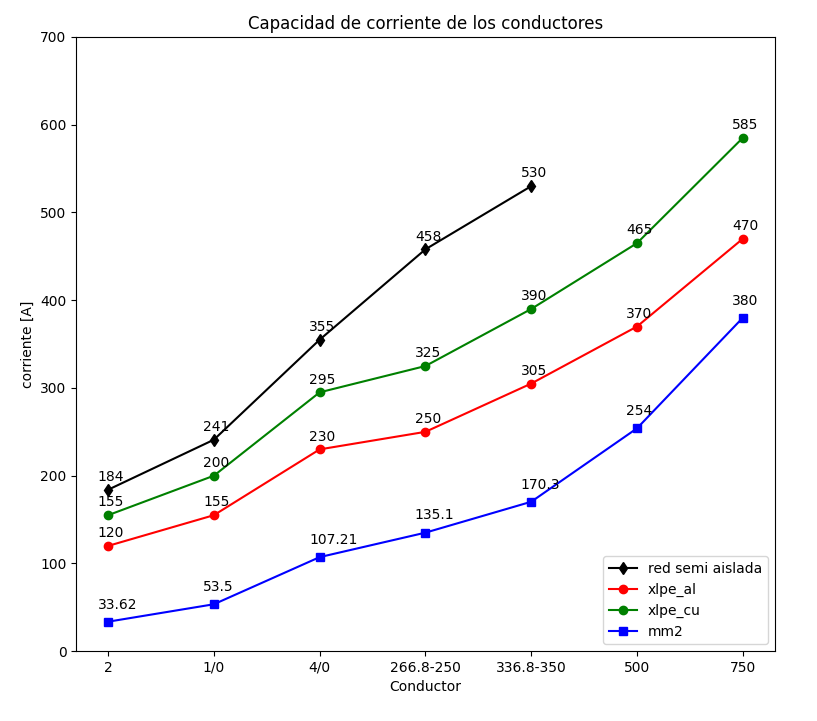
\includegraphics[width=\linewidth]{capacidad_corriete}
\end{figure}


\section{CARGABILIDAD DE LOS TRANSFORMADORES}

Para los transformadores de potencia, en ningún caso se debe superar el 100\% de la capacidad nominal de cada uno. La capacidad real operativa de cada transformador estará determinada por las condiciones
de funcionamiento de los sistemas de refrigeración \cite{MANOPEMCALI}.

\chapter{CONTINGENCIAS}


Una contingencia se refiere a una situación de emergencia donde se puede llegar a perder parte del sistema de potencia. El sistema de distribución debe estar en capacidad de seguir suministrando carga en caso de una de las siguientes contingencias \cite{EMCALI2007}:

\begin{enumerate}
	\item Pérdida de una subestación con dos o tres transformadores.
	\item Pérdida de una barra de 13.2 kV
	\item Pérdida de un transformador.
	\item Pérdida de un tramo de circuito.
	\item Pérdida de un interruptor de circuito.
	\item Pérdida del tramo subterráneo.
\end{enumerate}

\subsubsection{Pérdida de una Subestación con Dos o Tres Transformadores}

En caso de pérdida de una subestación estandard se pierden
aproximadamente 77 MVA de carga en 13.2 kV (con una cargabilidad del 91\%), las cuales deben ser atendidos por las subestaciones adyacentes mediante transferencias de carga  de carga en la red.\\\\
 En una subestación promedio, el valor esperado de carga en cada transformador de 41.75 MVA es de 38 MVA y en cada transformador de 28 MVA es de 26 MVA.\cite{EMCALI2007}.\\\\

En caso de realizar realimentaciones totales de una subestación , de acuerdo a la cargabilidad del momento se recomienda seguir el siguiente plan de contingencia:

\subsubsection{Pérdida de una Barra de 13.2 kV}

 transferir las secciones de los alimentadores a alimentadores de otras
subestaciones

\subsubsection{Pérdida de un Transformador}

\subsubsection{Pérdida de un Tramo de Circuito}

\subsubsection{Pérdida de un Interruptor de Circuito}

\subsubsection{Pérdida del Tramo Subterráneo}

\section{DESCONEXIONES PREVENTIVAS}

Cuando se presentan retardos en la entrada  en operación de líneas , transformadores u otros activos pertenecientes al \ac{STN} o \ac{STR},  de acuerdo al análisis eléctrico  realizado por el \ac{CND},  este ordenará la desconexión preventiva de la demanda de un \ac{OR} cuando se presentan los siguientes casos: \cite{CREG2242016} \\\\

\begin{itemize}
\item Se desconectará el 20\% de la carga cuando un evento no programado o contingencia sencilla  \footnote[1]{Cada uno de los eventos no programados que causan la no operatividad de una línea, un transformador o un banco de transformadores del STN o del STR.}  sobre un activo (linea , transformador u otro ) pueda 
  \end{itemize}

Cantidad de carga en MW que se desconectaría de las redes del SIN ante la ocurrencia de una contingencia resultante de la operación de los equipos de protección del sistema, actuación de esquemas suplementarios, apertura de elementos por superación de límites operativos de equipos declarados por los agentes o por las instrucciones operativas del CND derivadas de la ocurrencia de una contingencia. La desconexión correctiva de demanda es estimada por el CND, con base en la mejor información disponible para los análisis eléctricos.

\section{RESTABLECIMIENTO}

Los restablecimientos se desarrollan bajo el acuerdo CNO 1784 del 2013

\chapter{CALIDAD DEL SERVICIO}

La calidad del servicio  es una variable que representa las características técnicas del servicio que el usuario percibe. Esta afectada por los eventos que ocurren en
el \ac{SIN}, los cuales pueden o no dejar demanda no atendida.

\begin{figure}[H]
  \centering
  \caption{Evento de gran magnitud}
  \label{fig:eventogranmagnitud}
  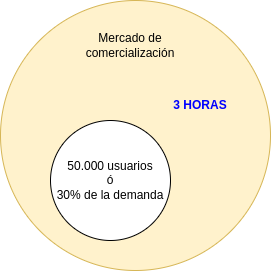
\includegraphics[width=0.6\linewidth]{evento_gran_magnitud}
\end{figure}

Es preciso indicar que las compensaciones por calidad se sustentan en fundamentos regulatorios
de acuerdo con el sistema o nivel de tensión.


\section{CALIDAD DEL SERVICIO EN EL STR}

Las definiciones de la calidad del servicio en el \ac{STR} son las siguientes:

\begin{itemize}
\item  \textbf{CNE} - Compensación por energía no suministrada: Compensación por ocasionar energía no suministrada o por dejar no operativos otros activos
\item \textbf{ENS} - Energía no suministrada: Estimación de la cantidad de energía que no pudo ser entregada cuando se presentan eventos en el sistema, realizada con base en las disposiciones que para tal fin se establecen en la regulación vigente.
\item \textbf{Indisponibilidad}: Se define como el tiempo durante el cual un activo de uso no estuvo en servicio total o parcialmente. Un activo estará indisponible, y se seguirá considerando en esta condición, aunque su función esté siendo suplida por otro activo del SIN.
\item \textbf{Disponibilidad}: Se define como el tiempo total sobre un período dado, durante el cual un activo de uso estuvo en servicio o cuando, sin estar en servicio, el agente lo declara disponible y el CND no instruye su conexión por condiciones de topología, seguridad, confiabilidad o calidad del SIN.
\end{itemize}


 Los siguientes  grupos de activos incluyen las bahías de conexión :\\\\
  \begin{itemize}
  \item Conexión del OR al STN
  \item Equipo de compensación
  \item Línea del \ac{STR}
  \end{itemize}

\subsection{Cambios del ingreso del OR por eventos en el STR}

El ingreso de cada agente se ve afectado por las siguientes variables:\\\\

\begin{itemize}
\item Cuando las in-disponibilidades superan las máximas horas anuales de in-disponibilidad ajustadas
\item Las in-disponibilidades debidas a catástrofes no superen los seis meses
\item La energía no suministrada no debe exceder los límites.
\item Un activo que supero las máximas horas de in-disponibilidad ajustada no se puede permitir que deje otros activos no operativos
\end{itemize}

\subsection{Plazos para los informes de eventos}
Para realizar los procedimientos descritos (eventos programados y no programados ) se tendrán en cuenta los siguientes plazos, cada uno contado a partir de las 24:00 horas del día de operación:\\\\


\begin{table}[H]
  \centering
  \caption{Tiempos de reportes}
\begin{tabular}{|p{4cm}|c|c|}
  \hline
Actividad & Responsable&Plazo (h)\\\hline
Ingreso de reporte de eventos &Agente&12\\\hline
Validación y publicación de listado de inconsistencias&
CND&
36\\\hline
Solicitud de modificación de información&
Agente&
60\\\hline
Respuesta a solicitudes de modificación&
CND&
72\\\hline
\end{tabular}
\end{table}

\subsection{Tiempos de indisponibilidad en el STR}

  Los siguientes grupos de activos utilizados en la prestación del servicio de distribución de energía eléctrica en el STR, no deberán superar, en una ventana móvil de doce meses, el número de máximas horas anuales de indisponibilidad, MHAI, que se definen para los grupos de activos identificados en la tabla \cite{CREG0152018}.\\\\


  \begin{table}[H]
    \centering
    \caption{Máximas horas anuales de  indisponibilidad  en el \ac{STR}}
  \begin{tabular}{|p{6cm}|c|}
    \hline
Grupos de Activos&
MHAI\\\hline
Conexión del OR al STN&
65\\\hline
Equipo de compensación&
18\\\hline
Línea del STR&
38\\\hline
Barraje sin bahías de maniobra&
15\\\hline
Barraje con bahías de maniobra&
30\\\hline

  \end{tabular}
\end{table}

En caso de un mantenimiento mayor el cual requiere más horas de las programadas en las máximas horas anuales de indisponibilidad, se tienen en cuenta las horas que se muestran en la figura \ref{fig:mayor} \cite{CREG0152018}.

    \begin{figure}[H]
      \centering
      \caption{máximas horas anuales de indisponibilidad para los mantenimientos mayores}
      \label{fig:mayor}
      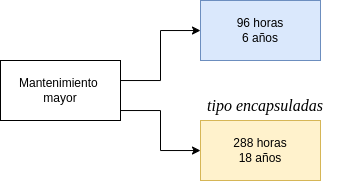
\includegraphics[width=\linewidth]{mantenimoento_mayor}
    \end{figure}
  

  Los reportes realizados por el \ac{OR} al \ac{CND} son los que se muestran en la figura:
  
\begin{figure}[H]
  \centering
  \caption{Reportes enviados al CND}
  \label{fig:reportes_transmision}
  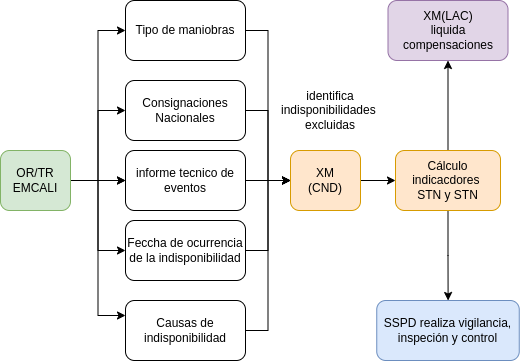
\includegraphics[width=\linewidth ]{reportes_transmision}
\end{figure}
  
   Las máximas horas anuales de indisponibilidad  se reducen en 0.5 h cuando se presenten unas de las siguientes situaciones:
  
  \begin{figure}[H]
    \centering
    \caption{incremento de las maximas horas anuales de indisponibilidad}
    \label{fig:mhaia}
    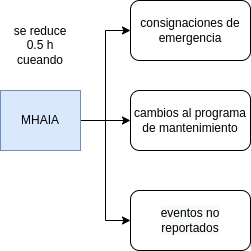
\includegraphics[width=0.6\linewidth]{MHAIA}
  \end{figure}

  
\section*{Ejemplo Numérico de las MHAI Ajustadas ($MHAI A_{m, gu}$)}

El ajuste de las máximas horas anuales de indisponibilidad se calcula para cada grupo de activos ($gu$) en el mes $m$ [1, 2].

\subsection*{Fórmula de las Máximas Horas Anuales de Indisponibilidad Ajustadas}

La fórmula para el ajuste es la siguiente, según la sección 5.1.6 de la resolución [1, 2]:

\begin{equation}
	\label{eq:mhaia}
	MHAI A_{m, gu} = MHAI_{gu} - 0,5 \cdot \left( \sum_{u=1}^{NGU} SCE_{m, u} + \sum_{u=1}^{NGU} CPM_{m, u} + \sum_{u=1}^{NGU} ENR_{m, u} \right)
\end{equation}

Donde [1, 2]:
\begin{itemize}
	\item $MHAI A_{m, gu}$: Máximas horas anuales de indisponibilidad ajustadas, calculadas para el mes $m$.
	\item $MHAI_{gu}$: Máximas horas anuales de indisponibilidad del grupo de activos $gu$.
	\item $SCE_{m, u}$: Número acumulado de solicitudes de consignaciones de emergencia (exceptuando las excluidas) para el activo $u$.
	\item $CPM_{m, u}$: Número acumulado de cambios al programa de mantenimientos (exceptuando los excluidos) para el activo $u$.
	\item $ENR_{m, u}$: Número de eventos o finalización de maniobras no reportados en los plazos establecidos, para el activo $u$.
	\item $NGU$: Número de activos que conforman el grupo de activos $gu$.
\end{itemize}

\subsection*{Datos del Ejemplo}

Seleccionaremos el grupo de activos "Conexión del OR al STN".

\begin{enumerate}
	\item $MHAI_{gu}$ (Máximas Horas Anuales de Indisponibilidad para "Conexión del OR al STN"): $60$ horas [3, 4].
	\item $NGU$ (Número de activos en el grupo $gu$): Supongamos $NGU = 3$.
	\item Valores de ajuste (para una ventana móvil de doce meses que termina en el mes $m$):
	
	\begin{center}
		\begin{tabular}{|c|p{2cm}|p{2cm}|p{2cm}|}
			\hline
			Activo ($u$) & $SCE_{m, u}$ (Consignaciones de Emergencia) & $CPM_{m, u}$ (Cambios a Programa de Mantenimientos) & $ENR_{m, u}$ (Eventos No Reportados) \\
			\hline
			$u=1$ & $2$ & $1$ & $0$ \\
			$u=2$ & $0$ & $0$ & $1$ \\
			$u=3$ & $1$ & $1$ & $0$ \\
			\hline
			\textbf{Sumatorias ($\Sigma$)} & \textbf{3} & \textbf{2} & \textbf{1} \\
			\hline
		\end{tabular}
	\end{center}
\end{enumerate}

\subsection*{Cálculo de $MHAI A_{m, gu}$}

\textbf{Paso 1: Calcular la suma de los eventos de ajuste (término entre paréntesis):}

\begin{align*}
	\sum_{u=1}^{NGU} SCE_{m, u} &= 2 + 0 + 1 = 3 \\
	\sum_{u=1}^{NGU} CPM_{m, u} &= 1 + 0 + 1 = 2 \\
	\sum_{u=1}^{NGU} ENR_{m, u} &= 0 + 1 + 0 = 1
\end{align*}

Suma total de ajustes: $3 + 2 + 1 = 6$

\textbf{Paso 2: Aplicar el factor de reducción de 0,5:}

$$ 0,5 \cdot \left( 6 \right) = 3 \text{ horas} $$

\textbf{Paso 3: Calcular $MHAI A_{m, gu}$:}

Sustituyendo en la Ecuación \ref{eq:mhaia}:
$$ MHAI A_{m, gu} = 60 \text{ horas} - 3 \text{ horas} $$
$$ MHAI A_{m, gu} = 57 \text{ horas} $$

El valor de las Máximas Horas Anuales de Indisponibilidad Ajustadas para el grupo de activos "Conexión del OR al STN" en el mes $m$ es de \textbf{57 horas}.

\subsection{Cálculo de indisponibilidad en el STR}
Las horas que un activo  se encuentra  in disponible durante un mes, se pueden calcular como \cite{CREG0152018}:

\[ HID_{m,u} = \sum_{x=i}^{n}(H_{i,u}*(1-CAPD_{i,u}))  \]

\subsection{Capacidad de los activos tras un evento en el STR}

    La \textbf{capacidad de los activos} tras suceder un evento queda establecido  como se muestra en la figura \ref{fig:capacidad} \cite{CREG0152018}:

    \begin{figure}[H]
      \centering
      \caption[capacidad]{Capacidad de los activos tras ocurrir un evento}
      \label{fig:capacidad}
      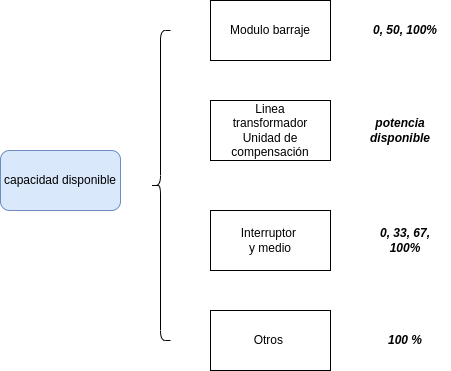
\includegraphics[width=\linewidth]{capacidad_eventos}
    \end{figure}




    \section{CALIDAD DEL SERVICIO EN EL SDL}

    \begin{figure}[H]
  \centering
  \caption{mapa conceptual del proceso de calidad del servicio}
  \label{fig:esquema}
  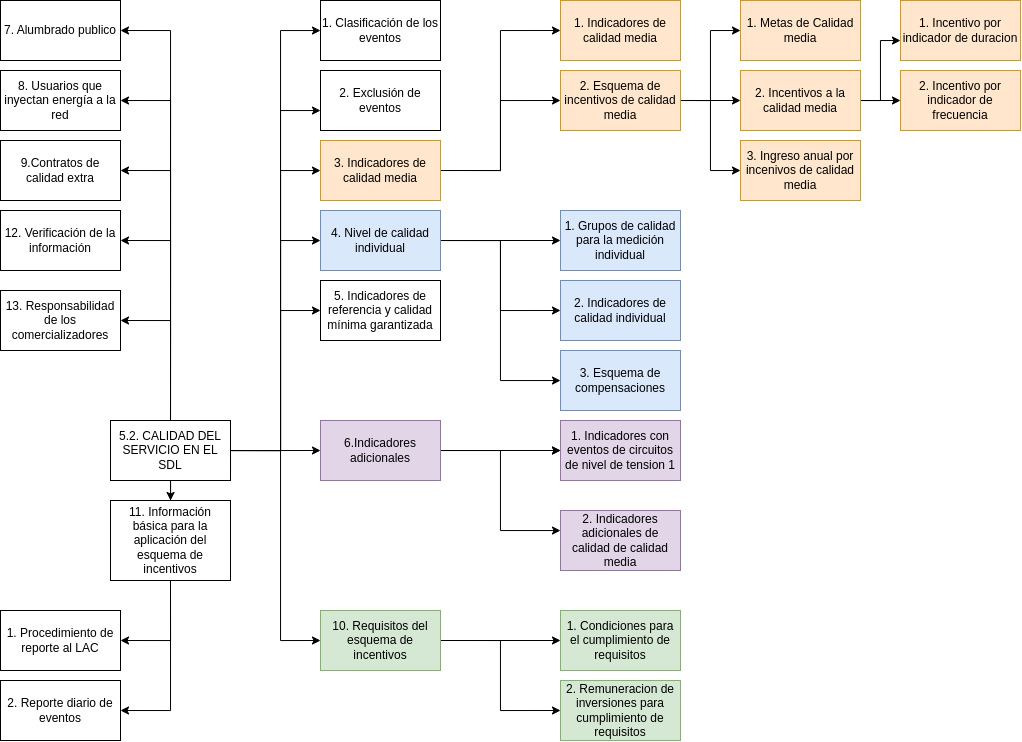
\includegraphics[width=\linewidth]{mapa_calidad_sdl}
\end{figure}

    El esquema de incentivos y compensaciones corresponde al nivel mínimo que deben cumplir las empresas dentro del plan regulatorio de metas para el mejoramiento de la calidad, el cual en concordancia con lo dispuesto por los artículos 58 y 59 de Ley 142 de 1994, estarán sujetos al seguimiento, vigilancia y control de la SSPD \cite{CREG0152018}.\\\\
    Para efectos de cumplir con la prestación continua de un servicio de buena calidad artículo 136 de la Ley 142 de 1994, o cualquier norma que la modifique o la adicione, los OR deberán abstenerse de incurrir en cualquiera de los siguientes escenarios \cite{CREG0152018}:

    \begin{figure}[H]
      \centering
      \caption{Eventos excluidos}
      \label{fig:excluidos}
      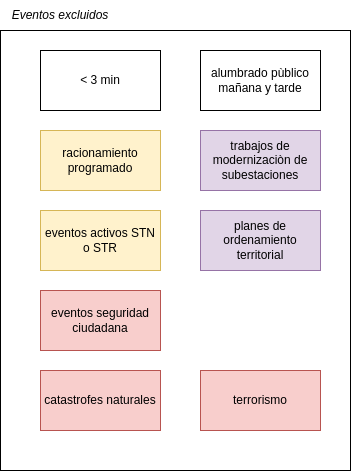
\includegraphics[width=\linewidth]{exclusiones_sdl}
    \end{figure}

    para su estudio los usuarios también se pueden agrupar en grupos
    de calidad lo cual depende de dos variables: los índices de
    ruralidad \textbf{IR} e índice de riesgo de falla \textbf{IRF},
    entonces se tienen seis posibles grupos de calidad como lo muestra
    la gráfica \ref{fig:gruposcalidad} \cite{CREG0152018}.\\\\

    \begin{figure}[H]
      \centering
      
      \caption{grupos de calidad}
      \label{fig:gruposcalidad}
      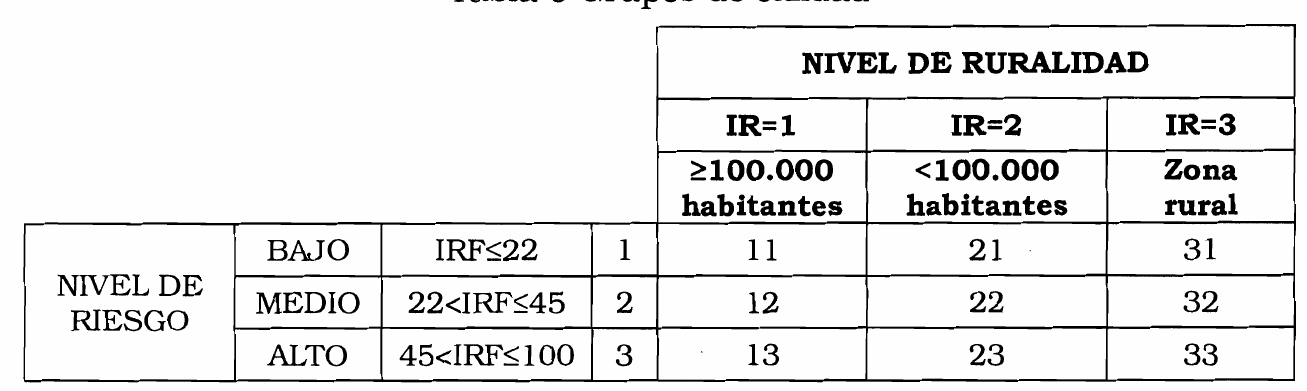
\includegraphics[width=\linewidth]{grupos_de_calidad}
    \end{figure}

    \section{INDICADORES DE CALIDAD DE DURACIÓN}

    La calidad  de energía  promedio o media del sistema en cuanto a duración puede ser establecida en función del indicador \textbf{SAIDI} (Indice de duración media de interrupción del sistema [\textit{System average interruption duration index}]) como se muestra a continuación:

    \[ SAIDI  = \sum_{m=1}^{12}\dfrac{\sum(D*NU)}{60*UT}   \left[  \dfrac{h}{usuario} \right]  \]\\
    Donde:\\\\
    \begin{tabular}[H]{p{1cm}p{8cm}}
      
      $D$ & {\small\it es la duración del evento en minutos}\\
      $NU$ & {\small\it es el número de usuarios afectados por el evento} \\
      $UT$ &  {\small\it  usuarios totales del \ac{SDL}} \\
    \end{tabular} \\\\

    Para determinar los valores a los que debe llegar se debe establecer las \textbf{metas anuales} para este indicador,  la cual se denomina \textbf{SAIDI\_M},  se parte de un valor  histórico de referencia denominado \textbf{SAIDI\_R}, para el caso de EMCALI  este valor es \textit{19.122 h} \cite{CREG0282020}.\\\\
    
    El indicador para medir la calidad individual anual para un usuario se conoce  como $DIU$, y el indicador mensual se conoce como $DIUM$ y se puede obtener a partir de:\\\\


    \[ DIU = \sum_{ma=m-11}^{m}DIUM  \]
    \[ DIUM = \sum_{i}^{IT}D\]
    En este caso la  duración del evento es en horas.\\\
    
    El valor  es límites que no se deberían sobrepasar se conocen como \textbf{DIUG}.\\\\

    Para los eventos momentáneos de debe calcular el \textbf{CAIDI}

    \begin{figure}[H]
      \centering
      \caption{Valores de SAIDI}
      \label{fig:valoressaidi}
      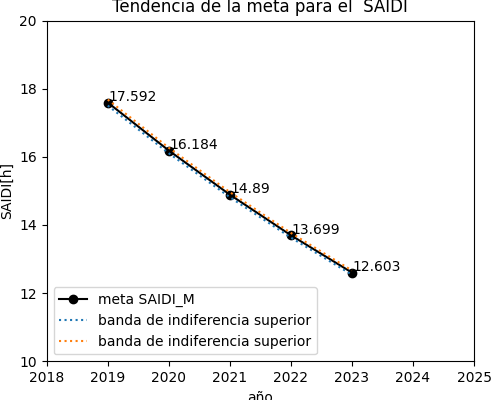
\includegraphics[width=\linewidth]{meta_saidi}
    \end{figure}
    
    \section{INDICADORES DE CALIDAD DE FRECUENCIA}
    
    \[ SAIFI  = \sum_{m=1}^{12}\dfrac{\sum(NU)}{UT}   \left[  \dfrac{veces}{usuario} \right]  \]

    Para elaborar los indicadores de calidad  individual de frecuencia se toma el de manera anual el $FIU$ y mensualmente el $FIUM$ como se muestra a continuación:\\\\

    \[  FIU = \sum_{ma=m-1}^{m} FIUM \]

    \[ FIUM = \sum_{i=1}^{IT} F\]

    El  valor límite que no se debería sobrepasar se conocen como  \textbf{FIUG}.

    Para los eventos momentáneos (nenores a 3 min) se debe reportar el \textbf{MAIFI} el cual se calcula como:
    \[ MAIFI = \dfrac{\sum_{i=1}^{n}NU }{UT}\]
    
    

    \chapter{PROTECCIONES ELÉCTRICAS}

    Las siguientes son las características generales de las protecciones eléctricas:\\\\
\begin{itemize}
	\item Alta Confiabilidad: Probabilidad de no omitir disparos
	\item Alta Seguridad: Probabilidad de no tener disparos indeseados
	\item Selectividad: Desconectar sólo lo fallado, evitando trasladar los efectos de las fallas a otros lugares del STN. 
	\item Rapidez: El tiempo de operación debe ser lo suficientemente corto de modo que garantice mantenerla estabilidad del sistema
        \end{itemize}

        En los sistemas eléctricos de los distribuidores, grandes consumidores y transportadores, el tiempo máximo de despeje de falla de la protección principal, desde el inicio de la falla hasta la extinción del arco en el interruptor de potencia, no debe
        ser mayor que 150 milisegundos.\\\\

        Los tipos de relés de sobre corriente se pueden clasificar como se muestra en la figura:

\begin{figure}[H]
      \centering
      
      \caption{tipos de relés en función al tipo de operación}
      \label{fig:tiporele}
      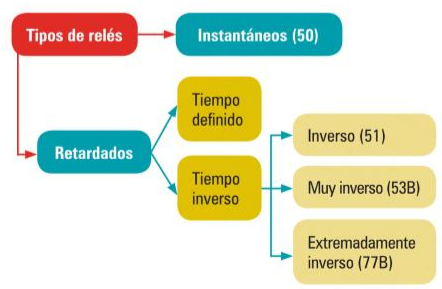
\includegraphics[width=\linewidth]{tipos_rele}
    \end{figure}



    \section{PROTECCIONES DEL TRANSFORMADOR}

    \begin{figure}[H]
      \centering  
      \caption{Protecciones del transformador de potencia}
      \label{fig:proteccionestrafo}
      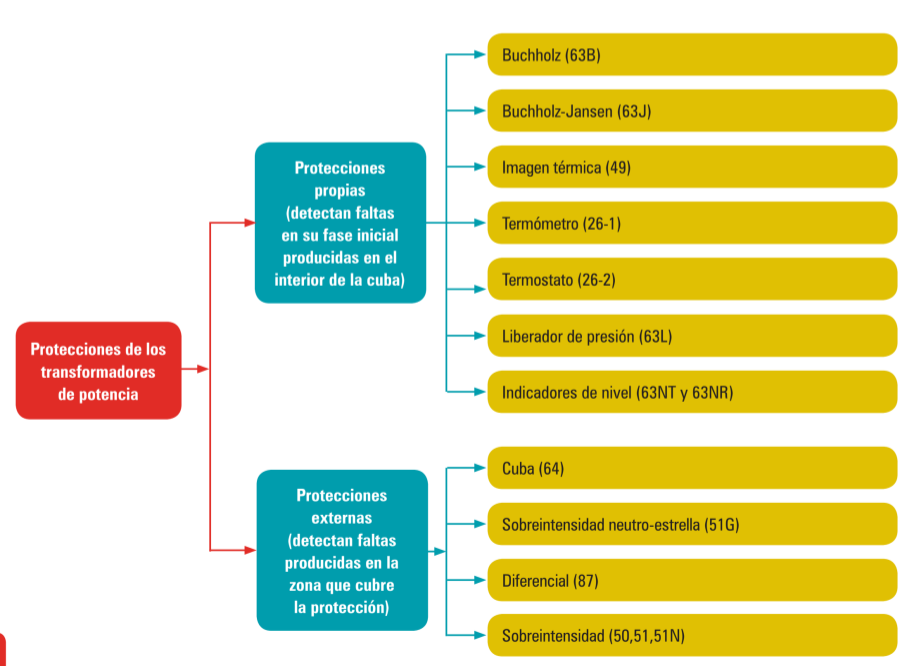
\includegraphics[width=\linewidth]{proteccion_trafo}
    \end{figure}

        \begin{figure}[H]
      \centering  
      \caption{diagrama protecciones del  transformador de potencia}
      \label{fig:diagramatrafo}
      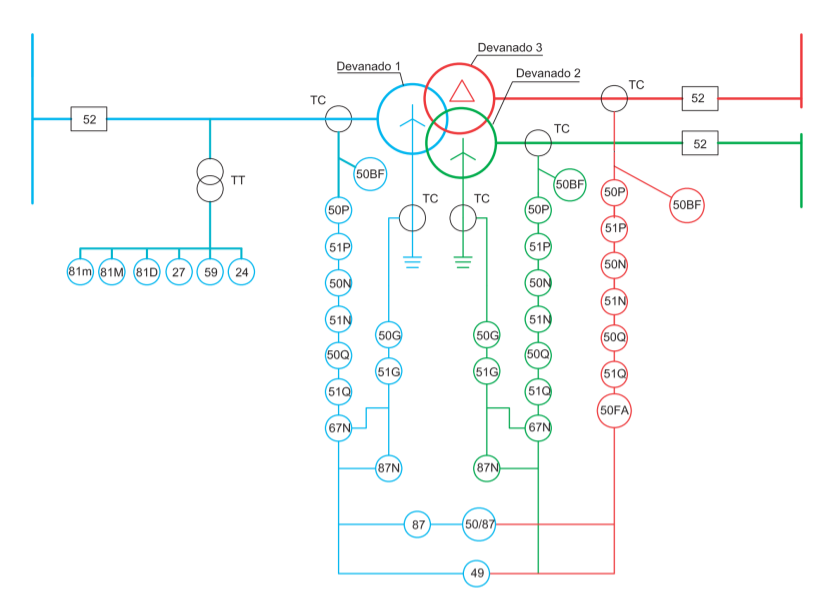
\includegraphics[width=\linewidth]{diagramapttrafo}
    \end{figure}

           \begin{figure}[H]
      \centering  
      \caption{diagrama protecciones del  transformador de potencia}
      \label{fig:diagramatrafo1}
      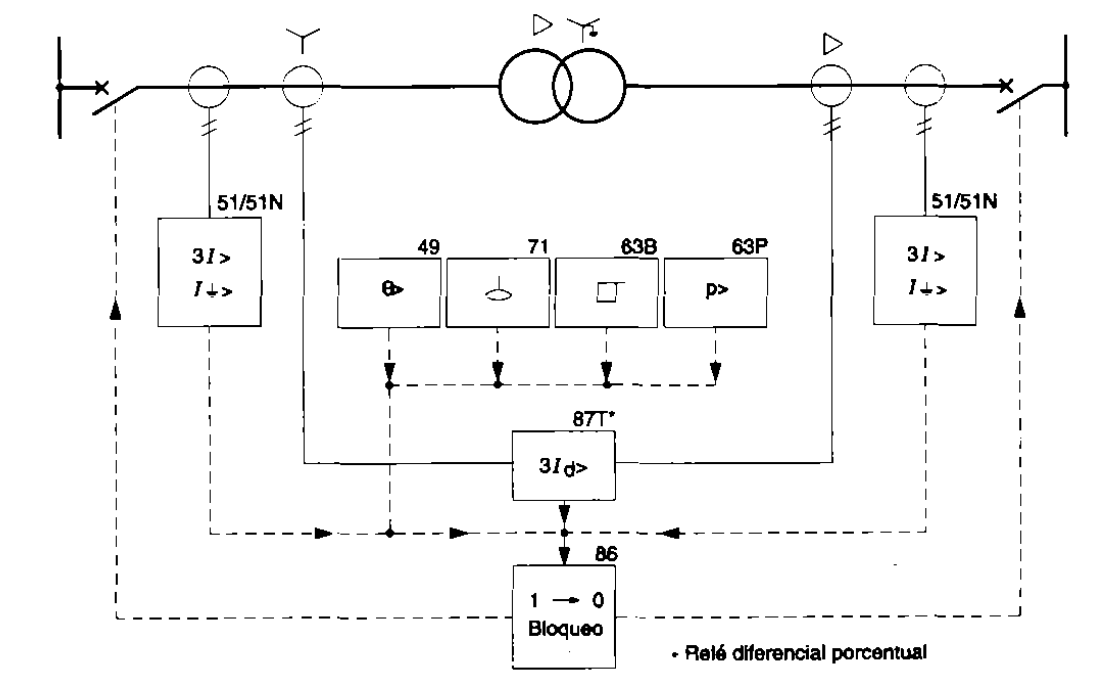
\includegraphics[width=\linewidth]{proteccion_trafo_1}
    \end{figure}

En la figura \ref{fig:zonas_diferencial},  se puestra el traslape de
zonas en la protección diferencial.
    
    \begin{figure}[H]
      \centering
      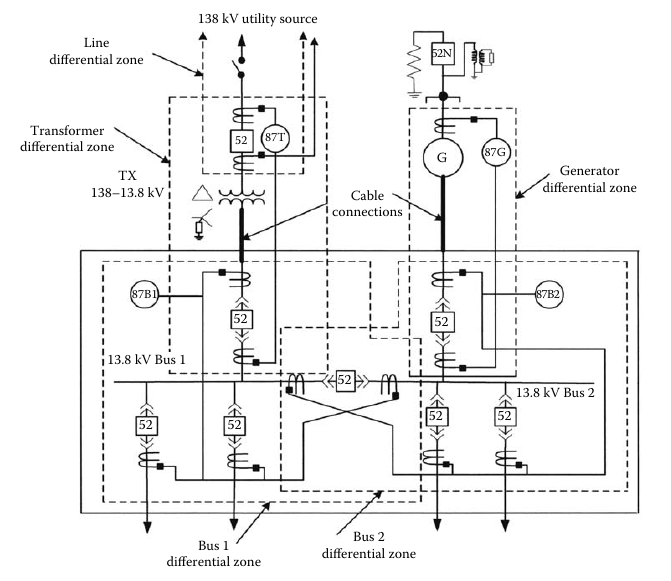
\includegraphics[width=\linewidth]{diferencial_tranformador}
      \caption{solapamiento de las zonas de protección diferencial}
      \label{fig:zonas_diferencial}
    \end{figure}
    



\begin{longtable}{|c|p{0.8\linewidth}|}
  \caption{Señales del transformador}\\
\hline \multicolumn{1}{|c|}{\textbf{Señal}} & \multicolumn{1}{c|}{\textbf{DESCRIPCIÓN}} \\ \hline 
\endfirsthead

\multicolumn{2}{c}%
{{\it \tablename\ \thetable{} -- continuación de la página anterior}} \\
\hline \multicolumn{1}{|c|}{\textbf{Señal}} & \multicolumn{1}{c|}{\textbf{DESCRIPCIÓN}}  \\ \hline 
\endhead
\hline \multicolumn{2}{|r|}{{\textit{Continua el la siguiente página}}} \\ \hline
\endfoot
\hline
\multicolumn{2}{|r|}{{ {\scriptsize\textit  fin de tabla}}} \\
\hline
\endlastfoot

  \small
  24 & Sobreexitación \\\hline
  23 & Temperatura \\\hline
  27 & Sub tensión \\\hline
  32 & Potencia direccional \\\hline
46 & secuencia negativa\\\hline
  49 & Térmico\\\hline
  50P & Sobre corriente instantánea de fase \\\hline
  50 & Sobre corriente \\\hline
  50BF & Fallo en breaker \\\hline
  50Q & Sobre corriente istantánea de secuencia negativa\\\hline
  51 & Sobre corriente de tiempo inverso \\\hline
  51Q & Sobre corriente inversa de secuencia negativa \\\hline
  50N & Sobrecorriente instantánea de neutro\\\hline
  50G & Sobre  corriente instantánea de de tierra \\\hline
  50FA& Sobre corriente con frenado de armónicos \\\hline
  55 & Factor de potencia \\\hline
  67 & Sobre corriente direccional\\\hline
  79 & recierre de CA \\\hline
  81M & Sobrefrecuencia \\\hline
  81m & Subfrecuencia \\\hline
  87N & falla restringida \\\hline
  86 & Rele de bloqueo \\\hline
  89 & interruptor de linea \\\hline
\end{longtable}

En el eje de las x es la corriente promedio de los devanados primario y secundario referida al primario. Indica la corriente de restricción llamada \textbf{Corriente de polarización}, Ib, mientras que la diferencia correspondiente en el eje Y representa la \textbf{corriente diferencial}. El relé de protección diferencial se activará si la magnitud de la corriente diferencial \textit{es superior a un porcentaje fijo de la corriente de restricción}.\\\\
  
    \begin{figure}[H]
      \centering  
      \caption{Curva del relé diferencial porcentual}
      \label{fig:proteccionestrafo}
      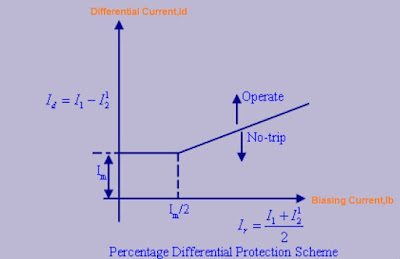
\includegraphics[width=\linewidth]{Proteccion-Diferencial-Porcentual}
    \end{figure}

    

\section{FUSIBLES}

La figura \ref{fig:tiposfusibles} muestra  los principales tipos de fusibles empleados en las redes de distribución.

\begin{figure}[H]
	\centering
	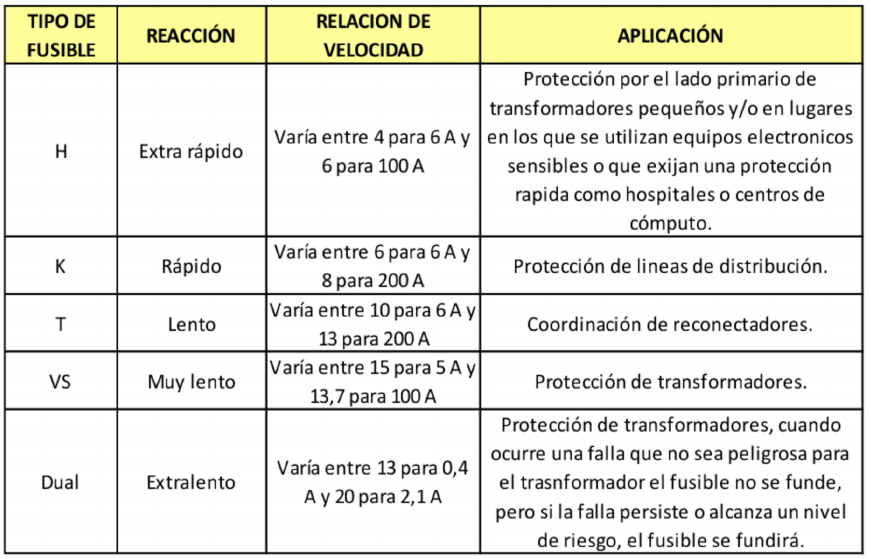
\includegraphics[width=0.7\linewidth]{tipos_fusibles}
	\caption{Tipos de fusibles empleados en media tensión}
	\label{fig:tiposfusibles}
\end{figure}


\chapter{MANTENIMIENTO}


\begin{figure}[H]
  \centering
  % \includegraphics[width=5]{}
  \caption{figura de prueba}
  \label{fig:prueba}
\end{figure}

\chapter{SISTEMAS DE  POTENCIA}

\section{FLUJO DE CARGA}
La potencia activa transmitida por una línea esta dada por la ecuación \ref{eq:1}:

\begin{equation}
  \label{eq:1}
  P=\dfrac{E_{1} \cdot E_{2} \cdot sen\delta } {X}
\end{equation}

En la figura \ref{fig:lineaat} se muestra una línea de transporte de alta tensión donde la impedancia de la línea \textit{$X$} se considera totalmente reactiva y los fasores de tensión  \textbf{$E_{1}$ }y \textbf{$E_{2}$} son las tensiones en la barra del transmisor y del receptor.\\\\

\begin{figure}[H]
  \centering
  
  \caption{Línea de transporte de alta tensión}
  \label{fig:lineaat}
  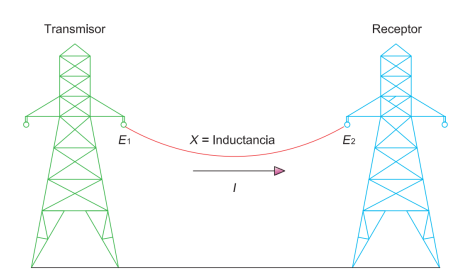
\includegraphics[width=\linewidth]{linea_transporte_AT}
\end{figure}

Entonces se puede obtener los flujos de potencia activa y reactiva
para los siguientes casos \cite{trashorras2015subestaciones}:

\begin{tabular}[H]{|p{0.2\linewidth}|p{0.35\linewidth}|p{0.35\linewidth}|}
  \hline
  CASO & Potencia \textbf{activa} & Potencia \textbf{reactiva}\\\hline
  Distintas magnitud de tensiones  y desfasadas. figura \ref{fig:caso1}  & El flujo de potencia activa siempre es de la tensión adelantada a la  retrasada& La linea absorve reactiva de ambos extremos\\\hline
  Distintas tensiones pero en fase. figura \ref{fig:caso2} & cero&la potencia fluye del nodo  de mayor tensión al de menor tensión y la línea absorve potencia reactiva  \\\hline
  Iguales tensiones pero desfasadas. figura \ref{fig:caso3}  &la línea transporta potencia activa proporcional a las perdidas &la línea absorve potencia reactiva de ambos extremos\\\hline
\end{tabular}


\begin{figure}[H]
  \centering
  \caption{Caso 1: esquema de flujo de potencia con tensiones distintas
    desfasadas.}
  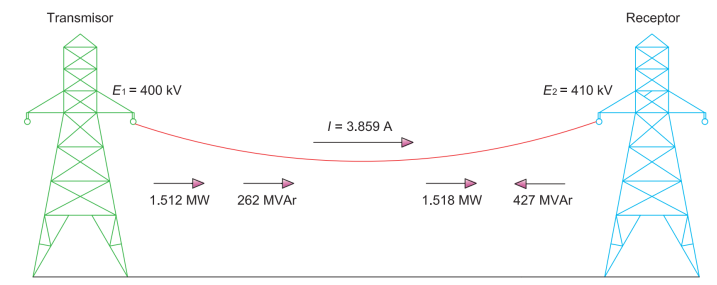
\includegraphics[width=\linewidth]{caso1}
  \label{fig:caso1}
\end{figure}


\begin{figure}[H]
  \centering
  \caption{Caso 2: esquema de flujo de potencia con tensiones distintas en
    fase.}
  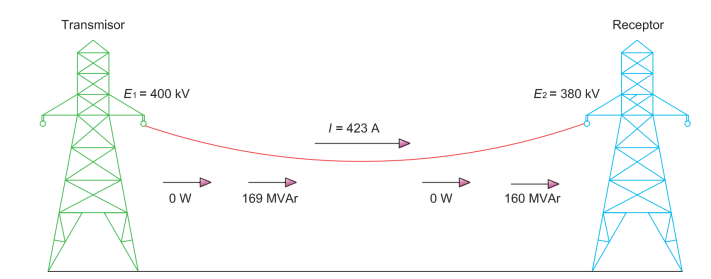
\includegraphics[width=\linewidth]{tensiones_distintas_igual_fase}
  \label{fig:caso2}
\end{figure}

\begin{figure}[H]
  \centering
  \caption{Caso 3: esquema de flujo de potencia con iguales tensiones
    desfasadas.}
  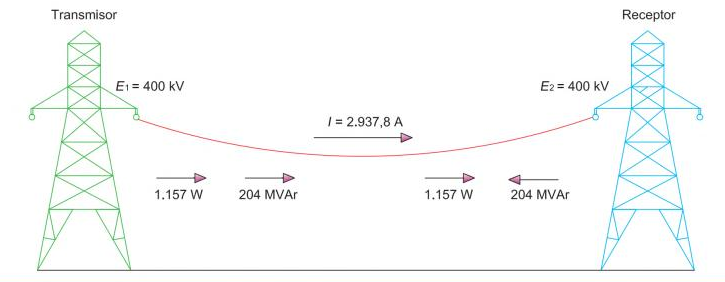
\includegraphics[width=\linewidth]{tensionesigualesdesfasadas}
  \label{fig:caso3}
\end{figure}

\section{CORTOCIRCUITO}

\begin{figure}[H]
  \centering
  \caption{fasores ante un corto circuito hacia adelante y hacia atraz}
  \label{fig:fasores}
  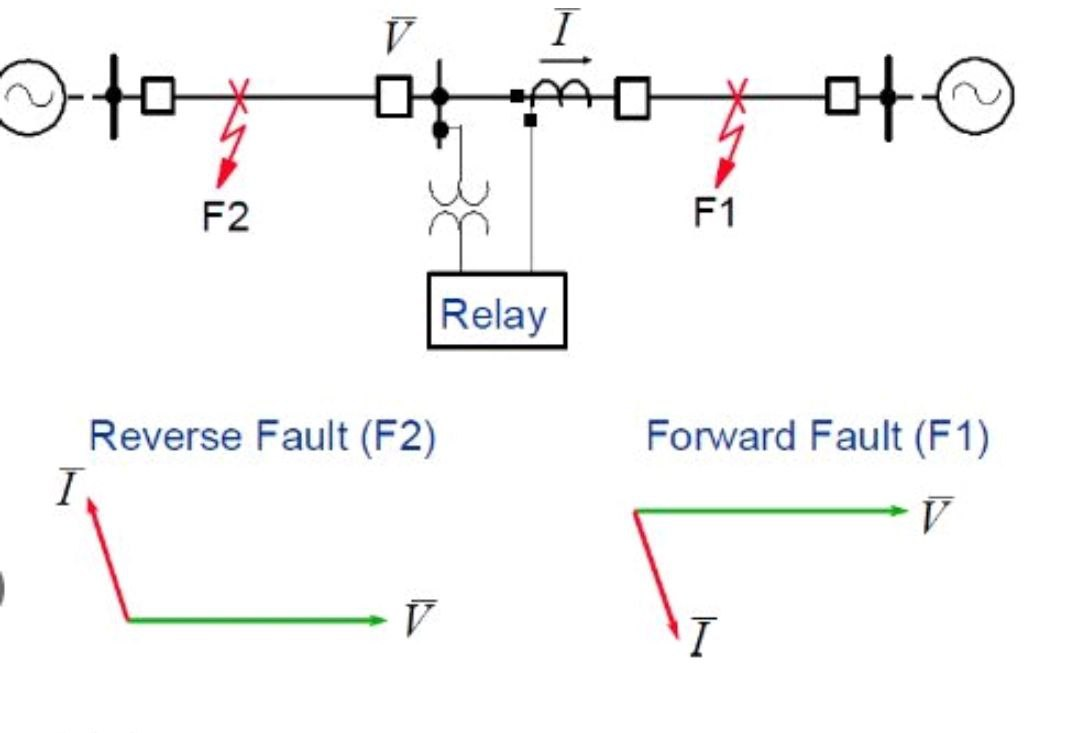
\includegraphics[width=\linewidth]{cortcircuito}
  \end{figure}

\chapter{PLANTAS FOTOVOLTAICAS}


La Resolución \textbf{CREG 030 de 2018}, o aquella que la modifique o la sustituya, define requerimientos para la conexión de los generadores de acuerdo con su capacidad instalada,
según los siguientes rangos:

\begin{enumerate}
	\item Conexión al STR o SDL del Autogenerador de Pequeña Escala (AGPE) con potencia 	instalada menor o igual a \textbf{0,1 MW} y Generación Distribuida (GD).
	\item  Conexión al STR o SDL del AGPE con potencia instalada mayor a \textbf{0,1 MW y menor o
	igual a 1 MW}.
	\item Conexión al STR o SDL del Autogenerador a Gran Escala (AGGE) con potencia instalada mayor a 1 MW y menor o igual a \textbf{5 MW}.
\end{enumerate}


La resolución \cite{CREG-060-2019} establece las normas para operación
de plantas fotovoltáicas, lo  cual implica cambios en los criterios de ajustes de protecciones, calidad de la potencia ,  control de tensión y despacho.\\\\

La resolución CREG 148 del 2021. Se reportan variables para plantas solares y fotovoltaicas.\\\\

\begin{itemize}
\item Acuerdos CNO 1521: Calidad de las vairiables reportadas.
\item
\end{itemize}

La generación distribuida  y la auto generación es tratada en la resolución CREG 030 del 2018 y sus limites son los definidos en la figura \ref{fig:gd}.

\begin{figure}[H]
	\centering
	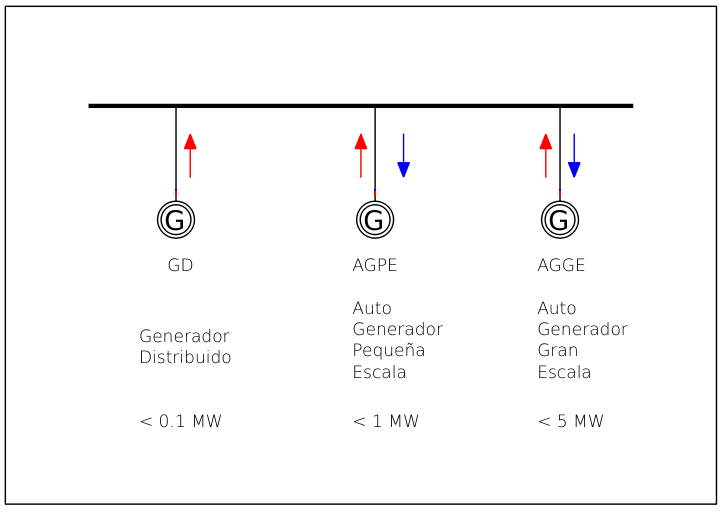
\includegraphics[width=0.7\linewidth]{gd}
	\caption{Capacidad de la auto generación y la generación distribuida}
	\label{fig:gd}
      \end{figure}
      
\chapter{SISTEMA DE GESTIÓN DE CALIDAD}

\chapter{ELEMENTOS DE UNA SUBESTACIÓN}

\section{TRANSFORMADORES}
\subsubsection{POLARIDAD}

La dirección relativa de los voltajes inducidos, que aparecen en los terminales de los devanados secundarios, depende del sentido en que estos terminales se enrollan dentro del núcleo  del transformador. Como los voltajes primario y secundario son inducidos por el mismo flujo mutuo, estos deben estar en la misma dirección. La forma en que aparecerán los voltajes inducidos como se ve desde los terminales del secundario depende de la dirección relativa de los devanados. La polaridad se refiere al orden definido en el que se sacan los terminales del tanque. La polaridad puede definirse como las relaciones vectoriales de voltaje de los cables del transformador extraídos del tanque. Con referencia a la figura \ref{fig:polaridadtransformadores}a, la polaridad es la dirección relativa del voltaje inducido de H1 a H2 en comparación con el de X1 a X2, ambos en el mismo orden.  \cite{POWERSADAS2012}\\\\
Cuando los devanados primarios y secundarios tienen el mismo sentido de arrollamiento se dice que tienen polaridad sustractiva, mientras que si el sentido del devano es opuesto se dice que las polaridades son aditivas.

\begin{figure}[H]
	\centering	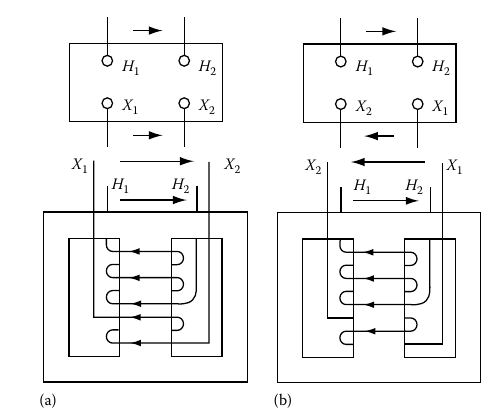
\includegraphics[width=0.7\linewidth]{polaridad_transformadores}
	\caption{Marcas de polaridad a) sustractiva b) aditiva}
	\label{fig:polaridadtransformadores}
\end{figure}

\subsection{Operación en paralelo de transformadores}

Para acoplar dos transformadores en paraleleo se deben tener en cuenta
los siguientes factores \cite{POWERSADAS2012}:

\begin{itemize}
\item La secuencia de fase debe ser la mísma.
\item La polaridad debe ser la misma.
\item La relación de tensiones debe ser la mísma
\item La impedancia de corto circuito debe ser la misma.
\end{itemize}

El reparto de carga en el transformador depende de la diferencia de
las impedancias de los transformadores:

\[ I_{1}= \dfrac{IZ_{2}}{Z_{1}+Z_{2}} \]

\[ I_{2}= \dfrac{IZ_{1}}{Z_{1}+Z_{2}} \]

Donde:

\begin{tabular}{ll}
  $I_{1} y I_{2}$ & Son las corrientes de fase de cada de cada transformador \\
  $I$& es la suma de las corrientes \\
\end{tabular}

\paragraph{Ejemplo}

\begin{figure}[H]
  \centering
  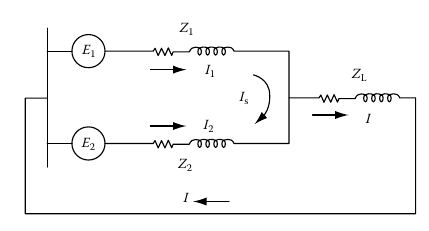
\includegraphics[width=\linewidth]{paralelo_trafo}
  \caption{circuito equivalente de circuito en paralelo}
  \label{fig:paralelo}
\end{figure}
Un transformador  de  10 MVA, 13.8–4.16 kV tiene una resistencia  y una reactancia en por unidad  de 0.005 y 0.05 , respectivamente. Este está en paralelo con un transformador de 5 MVA con la misma relación de transformación, y tiene una reactancia en por unidad de  0.006 y 0.04, respectivamente, calcule como pueden alimentar los dos una carga de 15 MVA con un factor de potencia de 0.8 en atrazo.

Convert Z1 and Z2 on any common MVA base and apply Equations C.14 and C.15. The results are as follows:

10 MVA transformer: S1 1⁄4 9.255 < 37.938
5 MVA transformer: S2 1⁄4 5.749 < 35.208

\section{PUESTA A TIERRA}

La resistencia de puesta a tierra es un indicador que limita directamente la
máxima elevación de potencial, pueden tomarse como referencia los valores máximos de la tabla \ref{tab:valorestierraretie}.

\begin{table}[H]
	\centering
	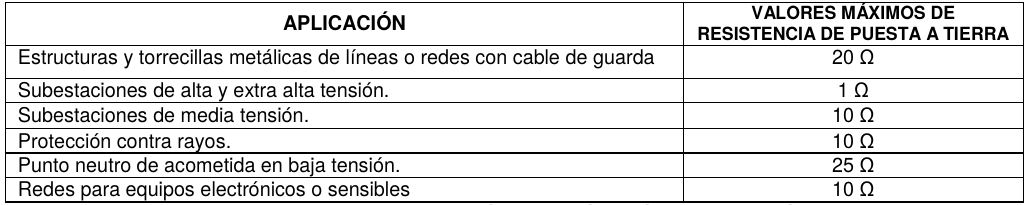
\includegraphics[width=0.7\linewidth]{valores_tierra_retie}
	\caption{Valores de puesta a tierra de acuerdo al RETIE \cite{RETIE2013}}
	\label{tab:valorestierraretie}
\end{table}

La forma como se conecta la tierra y el neutro esta determinado por el régimen de neutro , los cuales pueden ser del tipo TN, TT y TI. En la figura  \ref{fig:tnsystem} muestra los los sistemas  solidamente puestos a tierra. En al figura 

\begin{figure}[H]
	\centering
	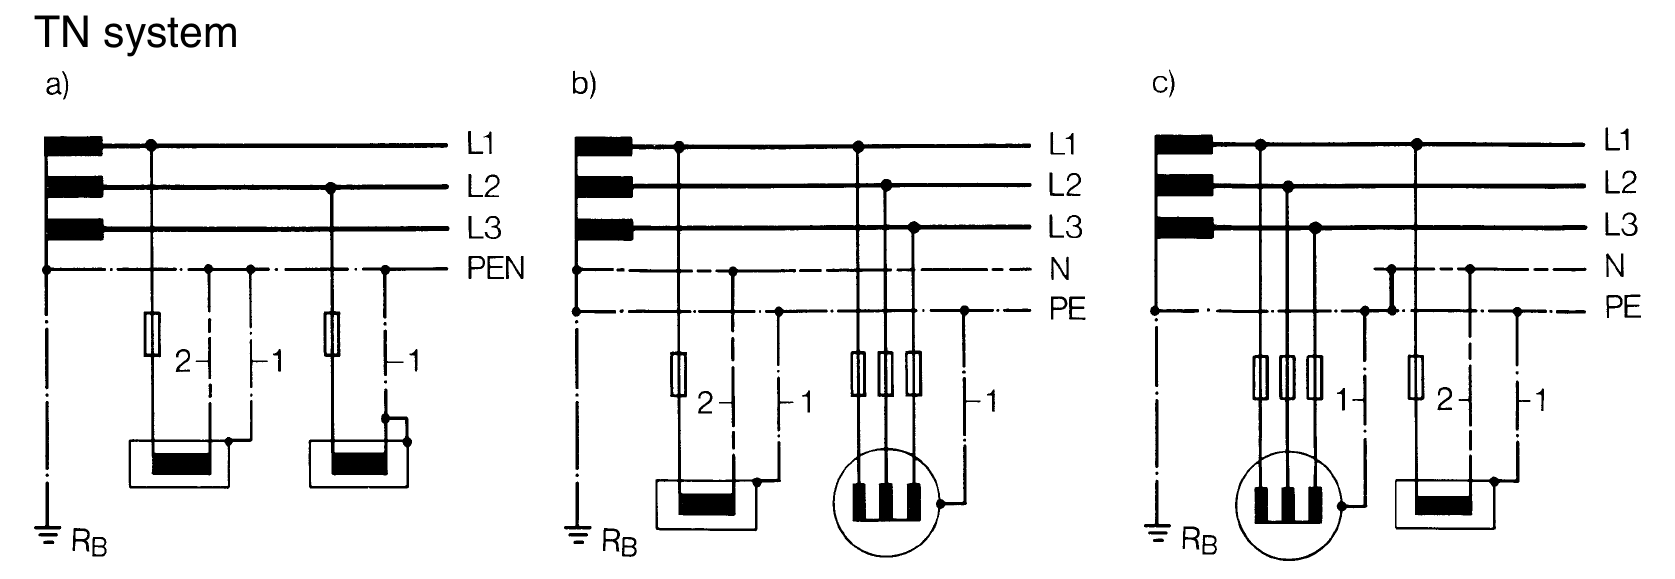
\includegraphics[width=0.9\linewidth]{tnsystem}
	\caption{Sistema TN,  a) TN-C tierra y neutro combinado, b) TN-S tierra neutro separado, TN-CS tierra neutro combinado separado }
	\label{fig:tnsystem}
\end{figure}


\begin{figure}[H]
	\centering
	%\includegraphics[width=0.9\linewidth]{../../../../../../..//home/alejandro/Pictures/tttisystem}
	\caption{Regimen TT y IT}
	\label{fig:tttisystem}
\end{figure}

\begin{table}
	\caption{Coordination of the type of earthing of the systems and protection devices
		}
	\centering
	\begin{tabular}{|c|c|}
		\hline
		Sistema &Dispositivos de protección\\\hline
		TN-S y TN-C-S &sobre corriente  y corrientes de falla\\\hline
		TN-C & sobre corriente \\\hline
		TT & sobrecorriente, corriente de falla\\\hline
		IT & sobrecorriente \\\hline
	\end{tabular}
	
\end{table}


\section{CÁMARAS DE  MEDIA TENSIÓN}
las dimensiones de las cámaras de media tensión son las siguientes (dimensiones en centímetros):\\

\begin{tabular}{|c|c|c|c|}
\hline
Inspección y desviación (0-30°) & 80&100&140 \\\hline 
Cámara de Tiro (T) & 120&230&180 \\\hline
Desviación 2 vías (D2) & 160&160&180\\\hline
Desviación 3 vías (D3) &160&230&180  \\\hline
Desviación 4 vías (D4) & 230&230&180 \\\hline
Maniobra (M) & 300&250&220  \\\hline
Transformación (TR) & 300&250&220  \\\hline
\end{tabular}

 \textbf{Inspección (I).}
Inspección y desviación (0-30°) de redes en media o media y baja tensión, donde solamente existe 1 nivel de conductos en media tensión. Incluye halado y empalme de redes en baja tensión.\\
La distancia máxima entre cámaras es de 60 metros, solo para circuitos en media tensión sin redes baja tensión y 40 metros para circuitos combinados de media y baja tensión.\\\\

\textbf{Tiro (T o TR100)}
Cámara de Tiro (T) para tiro, halado, empalme y desviación (0 – 45o) y transposición de cables para circuitos a 13.2 kV o cámara de inspección TR100 para circuitos a 34.5 kV que sirven de enlace entre subestaciones.\\


\textbf{Desviación 2 vías (D2)} Halado, inspección, empalme y desviación (45°-135°) de redes en media o media y baja tensión. Debe localizarse de acuerdo con la necesidad del proyecto específico.\\\\

\textbf{Desviación 3 vías (D3)}.
Halado, inspección, empalme y desviación (0-135°), 3 direcciones (en T), de redes en media y baja tensión. Debe localizarse sobre las intersecciones de vías en forma de " T " o de acuerdo con las necesidades del proyecto específico.\\\\
\textbf{Desviación 4 vías (D4)}
Halado, inspección, empalme y desviación (0 hasta ± 135°), 4 direcciones (en cruz), de redes en media o media y baja tensión. Debe localizarse en las esquinas,  o de acuerdo con las necesidades del proyecto específico.\\\\
\textbf{Cámara barraje (B2) o TR101}
Cámara B2 para instalar dos barrajes premoldeados a 13.2 kV o cámara TR101 para tiro, halado, empalme o transpocisión de cables de circuitos a 34.5 kV que sirven de enlace entre subestaciones.\\\\
\textbf{Maniobra (M)}
Halado, inspección, empalme y desviación (0-45°), de redes en media o media y baja tensión e instalación de una caja de maniobra (4 a 6 vías), 1 barraje premoldeado de 4 vías y motobomba. Debe localizarse de acuerdo con los datos básicos del proyecto y a la necesidad de equipos de maniobra.

\section{CONDUCTORES}

La capacidad de los conductores

\begin{figure}[H]
  \centering
  \caption{Listado de capacidad de los conductores}
  \label{fig:capacidaddeconductores}
  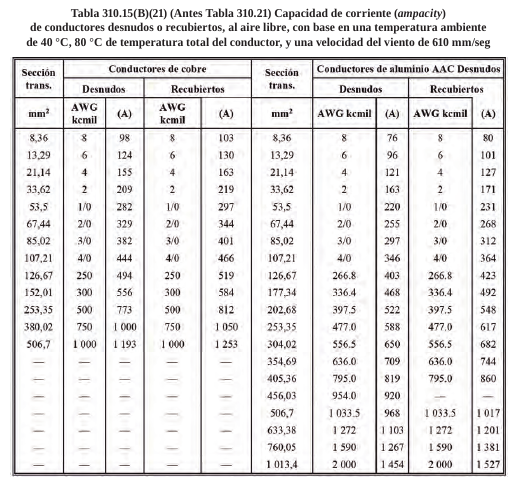
\includegraphics[width=\linewidth]{capacidad_cables_ntc_2050}
\end{figure}

\chapter{MONTAJE, INSTALACIÓN Y PRUEBAS ELÉCTRICAS}

\section{Pararrayos}

La conexión de los descargadores de sobretensiones a los
cortacircuitos se realiza , con conductor de cobre duro desnudo de
21.14 mm2 (4 AWG)Se utilizarán descargadores tipo óxido metálico de
Zinc

\begin{tabular}{|c|c|c|c|}
  \hline
  Parámetro& Unidad& 13.2 kV& 34.5 kV\\\hline
  Tensión& kV& 12& 30\\\hline
  Corriente de descarga&kA&10&10\\\hline
\end{tabular}

\section{TRANSFORMADORES}

En el caso de transformadores usados y o reparados éstos deben cumplir con los siguientes requerimientos para ser instalados:

\begin{enumerate}
	\item Tiempo de uso no mayor a 14 años (para transformadores usados).
	\item Fecha de fabricación posterior a 1985 (para transformadores reparados).
	\item Certificación de la procedencia del equipo.
	\item Certificación de que el equipo no presenta contaminación por bifenilos policlorados – PCB (resolución DG No. 601 de 2002 de CVC).
	\item  Protocolo de pruebas con las siguientes características.
	\begin{itemize}
		\item Datos de placa
		\item  Prueba de relación de transformación.
		\item  Prueba de resistencia de aislamiento
		\item  Prueba de resistencia de devanados y pruebas de pérdidas (vacío y carga).
	\end{itemize}
      \end{enumerate}

      \section{Pruebas a equipos eléctricos}

\begin{figure}[H]
	\centering
	\caption{Pruebas sobre transformadores}
	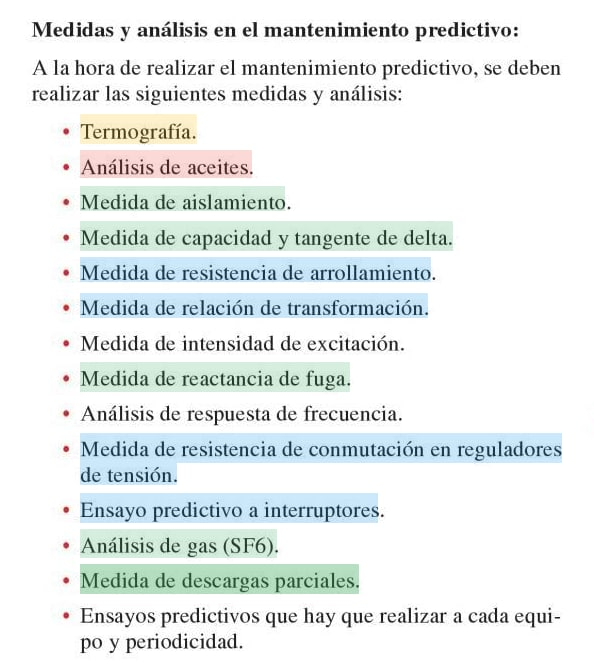
\includegraphics[width=0.7\linewidth]{pruebas}
	\label{fig:pruebas}
\end{figure}

\chapter{COMUNICACIONES Y CONFIGURACIONES}

\section{Acuerdos y regulación aplicable a las comunicaciones}

\subsection{Regulación}
La regulación aplicable a las comunicaciones es la siguiente:

\begin{itemize}
\item CREG 025 – 1995: Código de Redes, como parte del Reglamento de Operación del Sistema Interconectado Nacional
\item CREG 080 - 1999: Funciones de planeación, coordinación supervisión y control entre el Centro Nacional de Despacho (CND) y los agentes del SIN
\item CREG 060 - 2019: Reglamento de Operación para permitir la conexión y operación de plantas solares fotovoltaicas y eólicas en el SIN
\item CREG 148 - 2021: Conexión y operación de plantas solares fotovoltaicas y eólicas en el SDL con capacidad efectiva neta o potencia máxima declarada igual o mayor a 5 MW
\end{itemize}

\subsection{Acuerdos}

los acuerdos vigentes con relación a las comunicaciones son :

\begin{itemize}
\item 1411: Por el cual se aprueban los procedimientos y los indicadores relacionados con la Supervisión del SIN
\item 1428: Requisitos para la Prestación del Servicio de Regulación Secundaria de Frecuencia – AGC
\item 1525: Por el cual se aprueban los requisitos de la supervisión de las variables eléctricas de las plantas solares fotovoltaicas y eólicas en el SDL con capacidad efectiva neta o potencia máxima declarada igual o mayor a 5 MW
\item 1612: Puesta en operación de proyectos de transmisión que incluyan activos de uso del STN, STR, SDL y recursos de Generación
  \end{itemize}

\section{Informe de superación y enlaces CND}

  En cada punto a supervisar el valor será de 100\% si está supervisado, o 0\% si no está supervisado. Porcentaje de tiempo en que el Punto a Supervisar llega al sistema SCADA del CND. La meta CNO: 95\%, pero la meta del la CREG es 97 \%,  con periodicidad semanal. Para realizar este reporte se utiliza la plataforma GAO.

  De acuerdo a la resolución \textbf{CREG 083 de 1999} Por cada evento que se registre se debe enviar la fecha y hora con \textit{resolución de un (1) ms}, la identificación del elemento que cambió de estado y el estado. final del dispositivo.\\\\

  
Los protocolos de comunicaciones empleados en los sistemas eléctricos son los que se muestran en la figura \ref{fig:protocoloscomunicacion} de lo que se destaca la comunicación entre el \ac{OR} y el \ac{CND}, en que los OR se comunican con el \ac{CND} mediante el protocolo \textbf{ICCP} (\textit{Inter Control Center Communication Protocol}).

\begin{figure}[H]
  \centering
  \caption{Protocolos de comunicación en sistemas ecléctico}
  \label{fig:protocoloscomunicacion}
  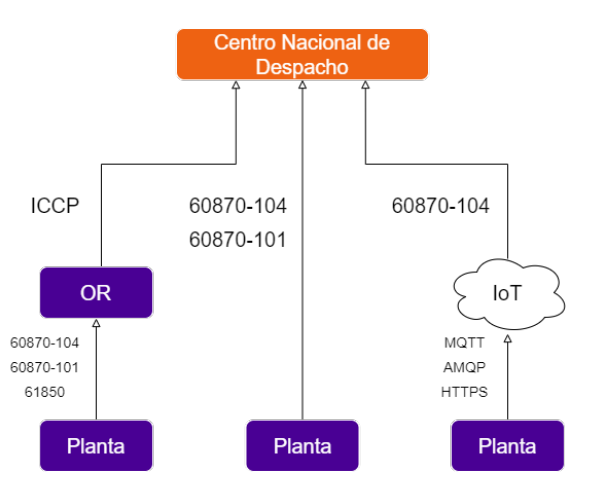
\includegraphics[width=0.5\linewidth]{protocolos_comunicacion}
\end{figure}

\section{ICCP}

El protocol ICCP  es basado en el concepto cliente servidor. Este protocolo se desarrolla en la capa 7 del modelo OSI. Todas las transferencias de datos se originan con una solicitud de un centro de control (el cliente) a otro centro de control que posee y administra los datos (el servidor). \texttt{Por ejemplo, si una aplicación del Centro de Control X necesita datos de la base de datos SCADA de Centro de Control Y, la aplicación Control Center X, que actúa como cliente, podría solicitar que Control Center Y, que actúa como servidor, envíe los datos en las condiciones especificadas por el cliente}.\\

\begin{figure}[H]
  \caption{Comunicación en la capa 7 para el protocolo ICCP}
  \label{fig:capa7iccp}
  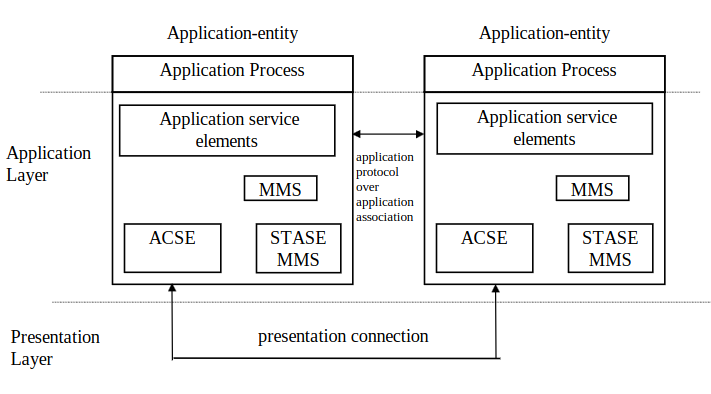
\includegraphics[width=\linewidth]{capas_iccp}
\end{figure}


El Association Control Service Element (ACSE) es un mecanismo utilizado por el protocolo ICCP (Inter-Control Center Communications Protocol) para el establecimiento de asociaciones lógicas entre un cliente y múltiples centros de control servidores\\\\
% Existen varios servicios proporcionados en \textbf{ICCP} para realizar transferencias de datos, según el tipo de solicitud. Por ejemplo, si el cliente realiza una solicitud única, los datos se devolverán como un respuesta a la solicitud. Sin embargo, si el cliente solicita la transferencia periódica de datos o la transferencia de datos solo cuando cambian, entonces el cliente establecerá primero el informe. El servidor (es decir, especificar condiciones de informes como la periodicidad de las transferencias periódicas u otras condiciones desencadenantes como el informe por excepción únicamente), y el servidor luego enviará los datos como un informe no solicitado siempre que se cumplan las condiciones de informe.\\\\
 

\section{ IEC 60870-5-104}

\begin{figure}[H]
  \caption{Introducción a IEC 61870 104}
  \label{fig:capa7iccp}
  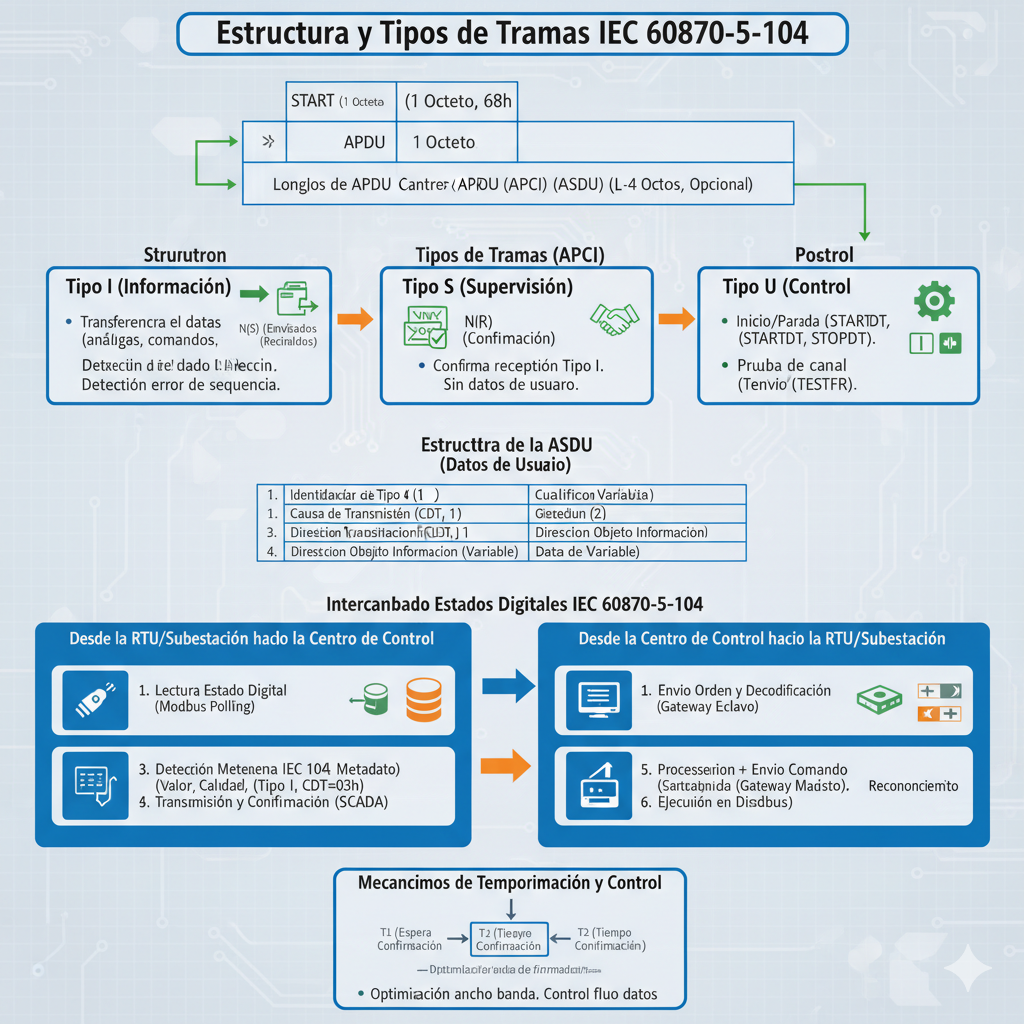
\includegraphics[width=\linewidth]{resumen_iec_61870_104}
\end{figure}

La trama de comunicación IEC 60870-5-104 se basa en la estructura de la \textit{Unidad de Datos del Protocolo de Aplicación} (\textbf{APDU}), y es una adaptación del protocolo \textit{IEC 60870-5-101} que utiliza \textbf{TCP/IP} para la comunicación en red.\\\\

La \textbf{APDU} se compone de dos partes principales: la \textit{Información de Control del Protocolo de Aplicación }(\textbf{APCI}) y, opcionalmente, la \textit{Unidad de Datos del Servicio de Aplicación} (\textbf{ASDU}), que contiene los datos de usuario.\\\\

La estructura de la \textbf{APDU} sigue un formato definido en la norma IEC 60870-5-104:\\\\


\begin{table}[H]
	\centering
	\caption{Contenido del APDU en el protocolo 60870-104}
\begin{tabular}{|p{0.3\linewidth}|p{0.45\linewidth}|p{0.15\linewidth}|}
  \hline
\rowcolor{black} \color{white}{Campo}&\color{white}Contenido& \color{white}Longitud (Byte)\\\hline
START&	Octeto de inicio&68h\\\hline		
Longitud de APDU (L)&Indica la longitud del resto de la trama (sin contar el START ni este campo)&1\\\hline
Campos de Control (APCI)	&Cuatro octetos que definen el tipo y control de la trama&	4\\\hline		
Datos de Usuario (ASDU)&Opcional, contiene la información de la aplicación& \\\hline
  \end{tabular}
\end{table}

  La longitud máxima de una APDU es de 253 byte.

  \subsection{Tipos de tramas (definidos por el APCI)}


  Los cuatro campos de control (APCI) (\textit{Control Field} en la figura \ref{fig:cabecera104})  son cruciales, ya que definen si la trama es de tipo \texttt{Información}, \texttt{Supervisión} o \texttt{Control} \cite{GOMEZ2019}.
  
  
\begin{figure}[H]
  	\centering
  	\caption{Formato del APCI}
  	\label{fig:cabecera104}
  	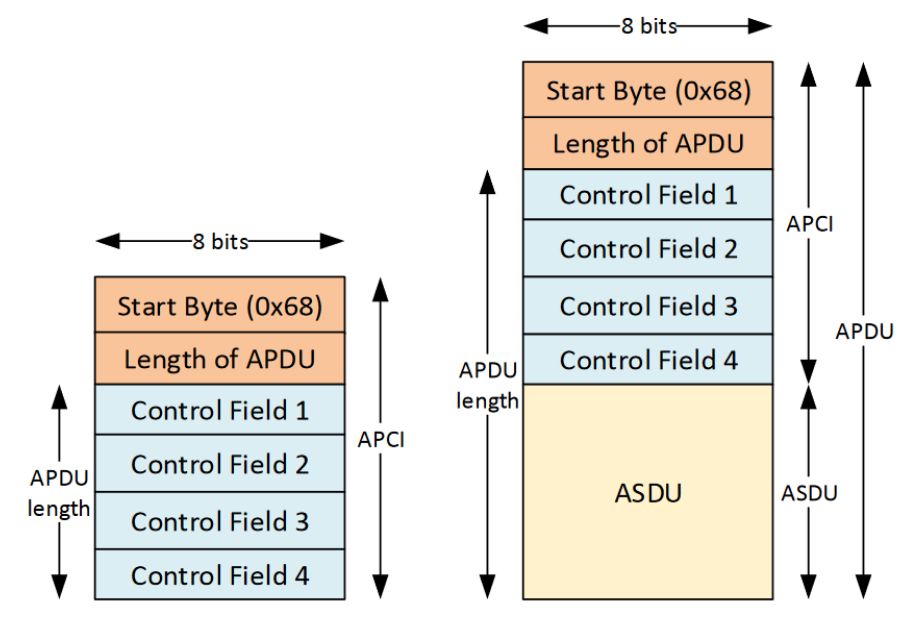
\includegraphics[width=0.7\linewidth]{cabecera_104}
\end{figure}

En la figura \ref{fig:tramas104} se discrimina los \texttt{control fiel} para tramas  del \textbf{APCI}.
  
\begin{figure}[H]
	\centering
	\caption{Tipo de APCI de IEC 60870-5-104}
	\label{fig:tramas104}
	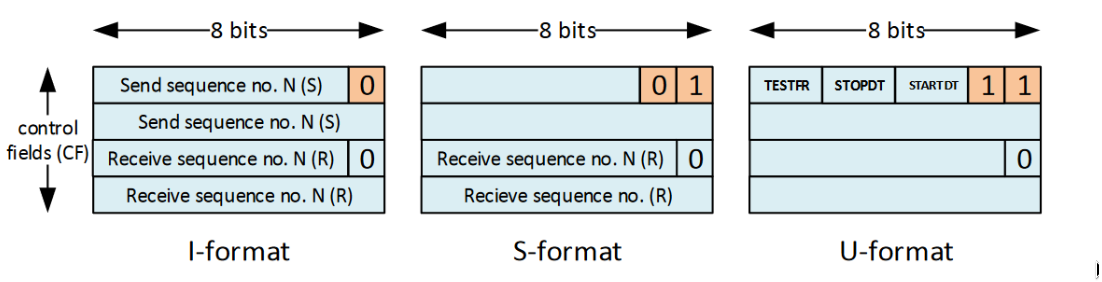
\includegraphics[width=0.7\linewidth]{tramas_104_}
\end{figure}
  

\begin{enumerate}
\item Tramas de Formato Tipo I (Información):
  \begin{itemize}
  \item Utilizadas para la transferencia de información del usuario.
  \item Contienen campos de secuencia de transmisión y recepción, denotados como N(S) (\textit{mensajes enviados}) y N(R) (\textit{mensajes recibidos y confirmados}).
  \item Permiten la comunicación de datos como señales analógicas o comandos.
  \item Si se pierde un mensaje, se detecta un error de secuencia y el canal puede cerrarse.
    \end{itemize}

\item Tramas de Formato Tipo S (Supervisión):
\begin{itemize}
\item Utilizadas exclusivamente para confirmar la recepción de tramas de \textbf{Formato Tipo I}.
\item No contienen datos de usuario (\textbf{ASDU})
\item La confirmación se realiza mediante el \texttt{campo de secuencia} \textbf{N(R)}, el cual indica el siguiente número de secuencia esperado, confirmando así todos los mensajes anteriores recibidos correctamente.
\end{itemize}

\item Tramas de Formato Tipo U (Control):
  \begin{itemize}
  \item Utilizadas para funciones de control, como el inicio o la detención de la transferencia de datos, o para verificar la actividad del canal
  \item Ejemplos de estas funciones incluyen el inicio de la comunicación (\texttt{STARTDT act/con}), la parada de la comunicación (\texttt{STOPDT act/con}) o el envío de una trama de prueba (\textit{test frame o señal de vida}) (\texttt{TESTFR act/con})
  \end{itemize}
  
\end{enumerate}


\subsection{Estructura de la ASDU (Datos de Usuario)}

\begin{figure}[H]
	\centering
	\caption{Formato ASDU}
	\label{fig:formatoasdu}
	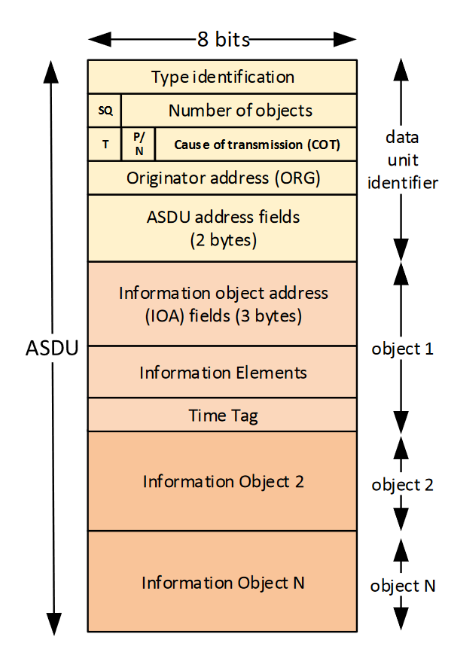
\includegraphics[width=0.7\linewidth]{formato_ASDU}
\end{figure}


Cuando la trama contiene datos de aplicación (Formato Tipo I), esta incluye una \textit{ASDU}. La \textit{ASDU} se compone de una \textit{unidad de identificación} (\textbf{data unit identifier}) y un \textit{objeto de información} (\textbf{objeto de identificacion}),  como muestra la figura \ref{fig:formatoasdu}.\\\\

La estructura simplificada de la \textbf{ASDU} es la siguiente:

\begin{enumerate}
\item Identificador de tipo \textit{type indentification} (1 BYTE): Determina la función de aplicación y la estructura del ASDU.
\item Cualificador de estructura variable (1 octeto): Generalmente vale 1.
\item Causa de Transmisión \textbf{cause of trasmission (CDT)} \ref{fig:formatoasdu} (1 byte): Indica por qué se transmite el mensaje (e.g., "solicitada", "activación", "confirmación").
\item Dirección Común del \textbf{ASDU} (2 byte): Identifica la estación terminal (ET) con la que se intercambia la información
\item Dirección del Objeto de Información (1 octeto): A menudo vale 0 en ciertas aplicaciones.
\item Datos de Información: Contiene los datos específicos de la aplicación (comandos, medidas analógicas, etc.)
\item El estándar IEC 60870-5-104 soporta una amplia variedad de datos en ambas direcciones (dirección monitor, desde la estación controlada hacia la controladora; y dirección control, desde la controladora hacia la controlada)
\item Mecanismos de Temporización y Control.

\end{enumerate}

Para garantizar una comunicación confiable, el protocolo utiliza mecanismos de temporización clave:

\begin{itemize}
\item Tiempos de Supervisión (\textit{T1, T2, T3, T0}): Estos tiempos controlan el flujo de datos y la actividad del canal.
\item \textit{Tiempo T3} (Tiempo de envío de trama de prueba): Si no se envía ningún mensaje durante el tiempo T3, se envía una trama de prueba (TESTFR) para verificar que el canal está activo
\item\textit{ Tiempo T2} (Tiempo de confirmación): Define cuánto tiempo debe esperar un receptor antes de enviar una trama Tipo S para confirmar mensajes recibidos
.
\item \textit{Tiempo T1} (Tiempo de espera de confirmación): Si se envía un mensaje Tipo I y no se recibe la confirmación (mediante una trama Tipo I o Tipo S que contenga el N(R) esperado) antes de que expire T1, se puede cerrar el canal o reintentar la comunicación
.
\end{itemize}

Estos mecanismos de control y temporización permiten que el protocolo 104 mejore el uso del ancho de banda al permitir el envío de múltiples mensajes de información (Tipo I) antes de requerir una confirmación explícita (Tipo S), a diferencia de comunicaciones seriales más antiguas.\\\\

\subsection{Intercambio de Estados Digitales IEC 60870-5-104}

El envío de un datos entre una RTU y el SCADA utilizando el protocolo IEC 60870-5-104 se realiza a través de (ASDUs) contenidas en tramas de Formato Tipo I.\\\\

La unidad de datos que intercambian el nivel de aplicación de una RTU y una SCADA se denomina ASDU (\textit{Aplication Service Data Unit}). Hay por lo menos un ASDU definido por cada tipo de \textit{punto de información} que se puede manejar con el protocolo. La identificación de un punto de información en este protocolo es por una dirección del punto \textit{IOA} (\textit{Information Objet Address}) más una dirección de común al \textbf{ASDU}, CAA (Common Address of ASDU).\\\\


Una conexión es un \textit{enlace TCP} con la estación controlada. A cada servidor se le pueden asociar varias conexiones que se pueden mantener conectadas. Así una conexión puede estar 
	\textbf{desconectada}, \textbf{conectada} y \textbf{activa}. Se considera activa cuando (estando conectada) la estación controladora habilita transferencia de datos para esa conexión. Todos los intercambios de ASDU son por la conexión activa. Dado que todas las conexiones se establecen por un mismo puerto TCP (2404) que establece la norma, la única forma de identificación de un servidor es por la dirección IP de la estación controlada. El que un servidor tenga más de una conexión se debe a la existencia de varios dispositivos de red o bien redundancia de equipo en el servidor.\\\\

A continuación, se describe este intercambio en ambas direcciones, basándose en el flujo de información en sistemas que utilizan este protocolo, como se ilustra en un sistema de pasarela de comunicación:

\subsubsection{Desde la RTU hacia el \textbf{SCADA} (Dirección Monitor)}
En esta dirección, el equipo (RTU) envía datos a la estación controladora (SCADA). Para un estado digital, la información se reporta como una indicación o evento. El flujo de información se inicia generalmente por un cambio de valor en el dispositivo de campo que debe ser reportado al centro de control:

\begin{enumerate}
\item \textit{Lectura del Estado Digital}: En arquitecturas de mediación como la pasarela 104, un componente llamado Control Maestro realiza un proceso periódico de lectura o "escaneo" (polling).
\item \textit{Detección de Evento} : Cuando el valor de una variable (p. ej., un bit) cambia en el dispositivo de campo (RTU), el Control Maestro consulta la Base de Datos de Intercambio, para determinar si el valor debe ser actualizado
\item \textit{Si el valor ha cambiado}, se considera que se ha generado un evento.
\item Mapeo del Metadato: La información actualizada se almacena en el Metadato, que contiene datos como el valor (True/False), la calidad (ej. Óptima) y, opcionalmente, una estampa de tiempo (time tag) asociada al momento exacto en que ocurrió el cambio.
\item \textit{Generación de la Trama IEC 60870-5-104}: El componente Control Esclavo (encargado de la comunicación IEC 104) mapea el Metadato a una trama IEC 60870-5-104 específica para el Centro de Control.
\item Si se trata de una indicación de 1 bit, se utiliza un tipo de dato como 	\textit{Single Indication} [1 Bit] with quality (o con estampa de tiempo). Si es una indicación de 2 bits, se utiliza \textit{Double Indication} [2 bit].
\item La trama contendrá un Identificador de tipo que indica que se transmite un objeto de información single (por ejemplo, 01h).
\item La Causa de Transmisión (CDT) indica que se ha generado un evento (p. ej., CDT = 03h).
\item Transmisión y Confirmación: La trama se envía al Centro de Control. El Centro de Control debe reconocer la recepción de la información.
\end{enumerate}

\subsubsection{Desde el Centro de Control hacia la RTU/Subestación (Dirección Control)}


En esta dirección, la estación controladora (SCADA) envía comandos para cambiar el estado de un dispositivo en la RTU.

\begin{enumerate}
\item \textbf{Envío de la Orden de Control (SCADA)}: El SCADA envía una trama IEC 60870-5-104 que contiene un comando para modificar el estado digital (p. ej., abrir o cerrar un interruptor). Para esto, se puede utilizar un \textit{Single Command} o \textit{Double Command}.
  
\item \textbf{Recepción y Decodificación (Control Esclavo)}: La RTU recibe y desempaqueta la información enviada por el SCADA.
  
\item \textbf {Búsqueda y Actualización de Metadato}: La RTU utiliza la \textit{dirección del objeto de información} (en la trama IEC 104) para buscar el \textit{Metadato} asociado en la Base de Datos de Intercambio. Este \textit{Metadato}, que puede tener asociado un comando (comando Modbus, por ejemplo), es actualizado con el nuevo valor de la orden de control.
  
\item \textbf {Procesamiento y Envío del Comando (Control Maestro)}: El Control Maestro toma el Metadato actualizado y lo procesa, encargándose de encapsular la información en el protocolo de la subestación (p. ej., IEC61850)
\item \textbf{Ejecución en el Dispositivo (IDE)}: El comando, ahora en el formato de protocolo local , es enviado al dispositivo de campo (RTU) indicado para su ejecución.
\item \textbf{Reconocimiento}: El dispositivo RTU retorna un reconocimiento de la escritura de la variable, que es gestionado internamente por el sistema (Control Maestro) y potencialmente notificado de vuelta al SCADA. Las tramas utilizadas para la transferencia de información del usuario, como los comandos y las indicaciones de estado digital, son de Formato Tipo I (Información), que contienen secuencias de transmisión y recepción.
\end{enumerate}


\subsubsection{Tipos de Datos}

Los datos de entrada:

\begin{itemize}
	\item \textbf{MSP}: Single-Point information.
	\item \textbf{MDP}: Double-Point Information.
	\item \textbf{MST}: Step position information.
	\item \textbf{MBO}: Bitstring of 32 bits.
	\item \textbf{MMEA}: Measured value, normalized value.
	\item \textbf{MMEB}: Measured value, scaled value.
	\item \textbf{MMEC}: Measured value, short floating point number.
	\item \textbf{MIT}: Integrated totals.
\end{itemize}

Los datos de salida:

\begin{itemize}
	\item \textbf{CSC}: Single command.
	\item \textbf{CDC}: Double command.
	\item \textbf{CRC}: Regulating step command.
	\item \textbf{CSEA}: Set-point command, normalizad value.
	\item \textbf{CSEB}: Set-point command, scaled value.
	\item \textbf{CSEC}: Set-point, command, short floating point number.
	\item \textbf{CBO}: Bitstring of 32 bits.
\end{itemize}

\subsection{Capa de aplicación}

\subsubsection{Funciones de Aplicación Principales}
\begin{itemize}
	\item \textbf{Definición:} Solicitudes que pueden enviarse entre el SCADA y la RTU.
	\item \textbf{Tipos de Funciones:}
	\begin{itemize}
		\item Secuencia de inicialización
		\item Adquisición de datos por polling (solo en Capa de Enlace, modo 101 desequilibrado)
		\item Transmisión de datos cíclicos
		\item Adquisición de eventos (espontáneos)
		\item Interrogación General (IG)
		\item Sincronización de reloj
		\item Envío de comandos
		\item Carga de parámetros
		\item Pruebas y transferencia de archivos
	\end{itemize}
\end{itemize}

\subsubsection{Adquisición de Datos}
\begin{itemize}
	\item \textbf{A. Interrogación General (IG)}
	\begin{itemize}
		\item \textbf{Propósito:} Sincronizar la base de datos del SCADA con los valores actuales de la RTU.
		
		\item \textbf{Alcance:}
		\begin{itemize}
			\item Todos los puntos (Interrogación General).
			\item Subconjuntos o grupos de puntos.
		\end{itemize}
		\item \textbf{Componente Clave:} \textbf{QOI (Calificador de Interrogación)} $\rightarrow$ Define el tipo de interrogación.
		\item \textbf{Secuencia Típica:}
		\begin{enumerate}
			\item \textbf{SCADA $\rightarrow$ RTU:} Envía IG (ASDU-100, COT 6 - Activación).
			\item \textbf{RTU $\rightarrow$ SCADA:} Responde con Confirmación (COT 7 - Act Con).
			\item \textbf{RTU $\rightarrow$ SCADA:} Envía múltiples ASDUs con los datos (COT 20).
			\item \textbf{RTU $\rightarrow$ SCADA:} Finaliza con Terminación (COT 10 - Act Term).
		\end{enumerate}
	\end{itemize}
	\item \textbf{B. Transmisión Autónoma (sin solicitud del SCADA)}
	\begin{itemize}
		\item \textbf{Transmisión Cíclica/Periódica:}
		\begin{itemize}
			\item Uso: Datos estáticos.
			\item Funcionamiento: La RTU envía datos periódicamente, incluso si no han cambiado.
		\end{itemize}
		\item \textbf{Adquisición de Eventos (Espontánea):}
		\begin{itemize}
			\item Uso: Cambios de datos.
			\item Funcionamiento: La RTU identifica un evento y lo reporta al SCADA.
			\item \textit{Nota: Es similar a "unsolicited response" de DNP3, pero en IEC 60870-5 el SCADA no puede deshabilitarla.}
		\end{itemize}
	\end{itemize}
	\item \textbf{C. Comando de Lectura (Read Command)}
	\begin{itemize}
		\item \textbf{Tipo de ASDU:} 102
		\item \textbf{Limitación:} Solo permite leer un único objeto por solicitud.
		\item \textbf{Recomendación:} Usar la Interrogación (IG) para leer múltiples objetos.
	\end{itemize}
\end{itemize}


\begin{figure}[H]
	\centering
	\caption{Secuencia de interrogación}
	\label{fig:secuenciadeinterrogacion}
	\includegraphics[width=\linewidth]{secuencia_de_interrogacion}
\end{figure}


\subsubsection{Controles y Comandos}
\begin{itemize}
	\item \textbf{Definición:} Solicitudes del SCADA para ejecutar una función (ej. enviar un comando de control de salida).
	\item \textbf{Secuencia de Control:} Similar a la IG, utiliza COT 6 (Activación), COT 7 (Confirmación) y COT 10 (Terminación).
	\item \textbf{Características:}
	\begin{itemize}
		\item Permite múltiples solicitudes simultáneas sin esperar respuesta.
		\item Las direcciones del punto de control y del punto monitorizado deben ser únicas.
	\end{itemize}
	\item \textbf{Mecanismo de Salidas (Control):} \textbf{Select-and-Execute}
	\begin{itemize}
		\item \textit{Equivalente a "Select-before-Operate" en DNP3.}
		\item \textbf{Pasos:}
		\begin{enumerate}
			\item SCADA envía \texttt{Select}.
			\item RTU confirma.
			\item SCADA envía \texttt{Execute}.
			\item RTU confirma la ejecución.
			\item Terminación del comando.
		\end{enumerate}
		\item \textbf{Calificadores de Comando:}
		\begin{itemize}
			\item Pulso corto
			\item Pulso largo
			\item Persistente (\textit{similar a "latched" en DNP3})
		\end{itemize}
	\end{itemize}
\end{itemize}

\begin{figure}[H]
	\centering
	\caption{Secuencia de comandos en capa de aplicación}
	\label{fig:comandos104}
	\includegraphics[width=1\linewidth]{comandos_104}
\end{figure}


\subsection{Ejemplo 104 - Reconectador}

\begin{figure}[H]
	\centering
	\caption{Diagrama de conexión del reconectador}
	\label{fig:reco104diagrama}
	\includegraphics[width=0.7\linewidth]{reco_104_diagrama}
\end{figure}

En el siguiente ejemplo se documenta la captura del trafico de un reconectador ( nodo \textit{522432} ) y el centro de control usando el protocolo \textit{IEC 60870-5-104}. En la figura \ref{fig:reco104} se muestra, a nivel de capa tres, que el reconectador usa la dirección \textit{IP 10.205.37.10}, mientras el centro de control emplea la dirección \textit{172.24.48.22}. En cuanto a la capa cuatro se observa que se emplea el protocolo TCP  con el puerto \textit{2404} en el reconectador y el puerto \textit{55464} en el centro de control. 

\begin{figure}[H]
	\centering
	\caption{Tramas capturadas de reconectador en el protocolo IEC 6070-5-104}
	\label{fig:reco104}
	\includegraphics[width=\linewidth]{reco_104}
\end{figure}

En el caso del tipo de tramas se pueden observar al inicio dos tramas tipo S, luego una trama tipo U, dos tramas mas tipo S y dos tramas tipo I y así sucesivamente en la columna \textit{Length info} de la figura \ref{fig:reco104}.\\\\

Para la última trama tipo I, se observa igualmente que la dirección global del ASDU en el campo \textit{Addr} es \textbf{104}. Por otra parte las dirección de objeto es IOA son 13002, 13003, 13003, etc.


\section{IEC 61850}

En la automatización de subestaciones, se reconoce como dos niveles :

\begin{itemize}
\item nivel de estación.
\item nivel de bahía.
\end{itemize}

En cuanto a los buses de comunicación tenemos:

\begin{itemize}
	\item Bus de estación (\textit{station bus}) x de 10 a 1GB se caracteriza por comunicar las MU (\textit{Merging Unit}) ó los concentradores de medidas con los relés de la estación.
    \item Bus de proceso se caracteriza por comunicar las MU (\textit{Merging Unit}) ó los concentradores de medidas con los relés de la estación.
\end{itemize}

\begin{figure}[H]
  \centering
  
  \caption{Estructura de redes de comunicación del protocolo IEC61850}
  \label{fig:iec61850}
  \includegraphics[width=\linewidth]{iec61850}
\end{figure}



\subsection{Modelo de Datos IEC 61850}

El modelo de datos IEC 61850 es una representación jerárquica de la información dentro de un IED (Dispositivo Electrónico Inteligente). Su propósito es estandarizar la comunicación y el intercambio de información en sistemas de automatización de subestaciones.

\begin{figure}[H]
  \centering
  \caption{Estructura IEC61850}
  \label{fig:iec61850}
  \includegraphics[width=0.5\linewidth]{anatomia_iec}
\end{figure}

\begin{figure}[H]
  \centering
  \caption{Estructura IEC61850 esquema gráfico}
  \label{fig:iec61850_ln}
  \includegraphics[width=0.7\linewidth]{LNs}
\end{figure}

\paragraph{Estructura Jerárquica}

\begin{enumerate}
\item     Dispositivo Lógico (Logical Device): El nivel superior del modelo, una colección de múltiples nodos lógicos.
    
\item Nodo Lógico (Logical Node): Modela las  aplicaciones y contienen objetos de datos.
    
\item Objeto de Datos (Data Object): O data de acuerdo a la figura \ref{fig:iec61850} están dentro de los nodos lógicos, su estructura está definida por la Clase de Datos.
    
\item Atributo de Datos (Data Attribute): es donde se encuentran los valores de los data objects.
  \end{enumerate}

\subsubsection{ Dispositivo Lógico (Logical Device)}

Estan definidos principalmente por el fabricante más que por la norma IEC 61850 y hacen referencia a los IDEs. De acuerdo a la figura \ref{fig:iec61850} hace referencia a Relay1.

\subsubsection{Nodo Lógico (Logical Node - LN)}

Es el elementos clave para modelar los elementos que componen los sistemas de comunicación, protecciones y automatización (ej. el elemento de la protección de distancia, interfaz a un seccionador).\\\\

Los nombres son estandarizados con cuatro caracteres. El primer carácter indica el grupo  (ej. P para protección, X para los equipos de maniobra). Los nodos se agrupan en grupos funcionales:

\begin{table}[H]
  \centering
  \label{Ejemplos de nodos Lógicos}

  \small
  \begin{tabular}{|p{0.2\linewidth} | p{0.2\linewidth}|p{0.5\linewidth}|}
    \hline
    \rowcolor{black}
    \color{white}{Grupo funcional} & \color{white}{Designación} &\color{white} {Nodos típicos} \\\hline
    System & Lxxx & \textbf{LLN0} (Datos de placa del IDE) \\\hline
    Automatic Control & Axxx & \textbf{ATCC} (Cambiador de tomas) \\\hline
    Control & Cxxx & \textbf{CSWI}  (Control de switches)  \\\hline
    Generic Functions & Fxxx & \textbf{FSCH} (funciones programadas) \\\hline
    Interfacing and Archiving & Ixxx & IHMI (representa el sistema SCADA) \\\hline
    Metering  and measurements & Mxxx & MMXU (medidas voltajes corrientes  o frecuencias) \\\hline
    Protection & Pxxx & \textbf{PDIS} (protección de distancia) \textbf{PTUV} (protección de bajo voltaje) \textbf{PDIR} (protección direccional) \textbf{PIOC} (protección de sobre corriente)\\\hline

    Power Quality & Qxxx & \\\hline
    Supervision & Sxxx & \textbf{SLTC} (supervición del OLTC) \textbf{SSWI} (supervición de switches) \textbf{SPTR} (supervición a transformadores de potencia) \\\hline

    Transformador de instrumento & Txxx  & \textbf{TCTR} (transformadores de corriente) \textbf{TVTR} (transformadores de voltaje) \\\hline

    Switchgear & Sxxx & \textbf{XCBR} (interruptor) \textbf{XSWI} (seccionador) \\\hline
   
    \end{tabular}
  \end{table}

\begin{figure}[H]
  \centering
  \caption{Ejemplo de nodos lógicos dentro de la subestación GIS }
  \label{fig:ln_example}
  \includegraphics[width=\linewidth]{ln_example}
\end{figure}


  
  \begin{figure}[H]
  \centering
  \caption{Restricción protocolo IEC61850}
  \label{fig:iec61850resticcion}
  \includegraphics[width=\linewidth]{restricciones}
\end{figure}

\subsubsection{Clase de Datos Común (\textit{Common Data Class} - CDC)}

Es como una \textit{"superclase"} (una clase madre que agrupa otras clases) que define qué atributos de datos están disponibles para un objeto de datos las cuales las agrupada según sus características principales (ej. SPS para estado de un solo punto, MV para valores medidos, DPC para control de doble punto).  Definidas en la parte 7-3 del estándar. La especificación incluye una lista de atributos de datos, el tipo de atributo (básico o clase de atributo construida), restricción de función, condición de presencia y posibles rangos de valores.\\\\
Ejemplo: INS es una CDC para información de estado de enteros; DPC es una CDC para control de doble punto.

\subsubsection{Objeto de Datos (Data Object - DO)}

Componente de un Nodo Lógico. La Clase de Datos Común (CDC) define la estructura y atributos de los data objects.Un objeto de datos (DO) puede tener múltiples \textit{atributos}. También puede contener sub-objetos de datos (que a su vez son de otras Clases de Datos Comunes).\\\\
Ejemplo:\\
El objeto de datos POS (posición de un interruptor) es de la Clase de Datos Común DPC (Double Point Control).\\\\
    Especificación: Definidos en las partes 7-4, 7-410 y 7-420 del estándar junto con los Nodos Lógicos. Incluyen un nombre, referencia a la CDC, explicación corta e indicación de obligatoriedad/opcionalidad.



\subsubsection{Atributo de Datos (Data Attribute - DA)}

    Definición: Las hojas de la jerarquía del modelo de datos donde se encuentran los valores.
    Tipos:Tipo Básico (Basic Type): Tipos de datos fundamentales (ej. entero de 32 bits sin signo, punto flotante). Definidos en la parte 7-2.
    Clase de Atributo Construida (Constructed Attribute Class - CAC): Atributos de datos que tienen una estructura interna, es decir, están compuestos por otros sub-atributos de datos (ej. Quality, Vector, AnalogValue, Timestamp).
    Restricciones de Función (Function Constraints - FC): Utilizadas para clasificar los atributos de datos según su propósito. Ejemplos:
    ST: Atributos de estado.
    CF: Atributos de configuración.
    SV: Atributos relacionados con sustitución.
    SP: Atributos de punto de ajuste (settings).
    Contenido: Los atributos de datos pueden ser de un tipo básico o tener niveles jerárquicos adicionales a través de Clases de Atributo Construidas hasta llegar a los componentes primitivos.

    \subsubsection{Clase de Atributo Construida (Constructed Attribute Class - CAC)}
    

    Definición: Un tipo de atributo de datos que posee una estructura interna, es decir, se compone de otros sub-atributos.
    Ejemplos: Quality (calidad de la información), Timestamp (marca de tiempo), Vector (magnitud y ángulo).
    Especificación: Definidas en la parte 7-3 del estándar.

Relación entre los Elementos y las Partes del Estándar

    Parte 7-4 / 7-410 / 7-420: Definen las clases de Nodos Lógicos, su semántica y la estructura en términos de Objetos de Datos, incluyendo nombres, descripciones semánticas y tipos.
    Parte 7-3: Define todas las Clases de Datos Comunes (CDCs) con su estructura en términos de Atributos de Datos (nombres, semántica, tipo). También define las Clases de Atributo Construidas (CACs).
    Parte 7-2: Especifica los tipos básicos y los tipos ACSI comunes.


    La configuración en el estándar IEC 61850 se basa en el uso de **archivos XML** a través del **Lenguaje de Descripción de Configuración de Subestaciones (SCL)**, definido en la parte 6 de la norma [1-6]. El SCL es la parte más importante de la serie IEC 61850 para el diseño de sistemas, ya que todo el proceso de ingeniería se puede apoyar en este lenguaje [2].

Los archivos SCL contienen información crítica del sistema y son fundamentales para el proceso de ingeniería, desde la especificación hasta el despliegue del sistema [3, 5, 7]. Se utilizan para describir las capacidades de los IEDs, el diseño del sistema y la configuración de la comunicación [3, 5, 8-11].


\subsection{Tipos de archivos }

Los principales tipos de archivo SCL empleados en la configuración de 61850 son:

\begin{enumerate}

\item {\textbf{SSD} (\textit{System Specification Description})}:Son el \textit{punto de partida inicial} en el proceso de ingeniería. Proporcionan información sobre la \textit{topología planificada} y los nodos lógicos (LN) requeridos para el sistema.

\item{\textbf{ICD} (\textit{IED Capability Description})}: Describen las capacidades genéricas de un Dispositivo Electrónico Inteligente (IED) específico. Son proporcionados por el fabricante y describen el modelo de datos y las capacidades de comunicación del dispositivo. Contienen una sección IED para el dispositivo cuyas capacidades representa. Antes de ser configurado, el nombre del IED en este archivo es típicamente "TEMPLATE".

\item {\textbf{IID} (\textit{Instantiated IED Description})}: Representan la \textit{funcionalidad de un archivo ICD parcialmente configurado}. En este archivo, el nombre del IED ya no es "TEMPLATE", sino que refleja el rol específico del IED en un esquema estándar.

\item{\textbf{CID} (\textit{Configured IED Description})}: Son archivos de configuración específicos.

\item{\textbf{SCD} (\textit{Substation Configuration Description})}: Son el \textit{resultado final del proceso de configuración} del sistema. Contienen toda la información necesaria para configurar un sistema de automatización de subestaciones . Pueden ser utilizados para una variedad de aplicaciones y son clave para la automatización y la puesta en marcha de los sistemas IEC 61850.

\item {\textbf{SIED} (\textit{System Interface Exchange Description})}:Se utilizan para el intercambio de datos entre herramientas de configuración de sistemas para diferentes proyectos de subestaciones. Son importantes para establecer comunicaciones entre subestaciones, fijando referencias de objetos de origen ya definidas y especificando nuevas conexiones de interfaz entre proyectos.

\end{enumerate}

Además de los archivos SCL, se utilizan otros tipos de archivos en contextos relacionados:

\paragraph{Archivos COMTRADE}: Se utilizan para el \textit{registro de perturbaciones} y para la grabación de perturbaciones basada en sincronofasores. Estos archivos son generados por los nodos lógicos relacionados con la protección.


\subsection{Protocolos empleados en IEC 61850}

En la figura \ref{fig:protocolosiec61850} se muestra la relación de los protocolos empleados en el estandard IEC 61850 y su relación con el modelo OSI.

\begin{figure}[H]
      \centering
      \caption{protocolos empleados en IEC 61850}
      \label{fig:protocolosiec61850}
      \includegraphics[width=0.7\linewidth]{cliente_servidor_61850}
    \end{figure}
    
    

\subsection{Arquitecturas}

\begin{figure}[h]
	\centering
	\caption{Arquitectura general de una subestacion}
	\label{fig:arquitecturasubestacion}
	\includegraphics[width=0.7\linewidth]{arquitectura_subestacion}
\end{figure}


\subsubsection{Anillo Sencillo}


\paragraph{Rapid Spanning Tree Protocol (RSTP)}

Definida en la IEEE 802.1w y IEC 62439-1 es recomendada para todos los mensajes exepto GOOSE  y Sampled Values.


\paragraph{Media Redundancy Protocol (MRP)}

Esta definida en la IEC 62439-2,  tiene tiempos de recpración bajos y puede ser usada con mensajes GOOSE.

\paragraph{High-availability Seamless Redundancy (HSR)}

Indicado en la IEC 62439-3 Clause 5,  no utiliza equipos intermedios y requiere que todos los dispositivos sean compatibles con esta arquitectura.\\\\ 

\begin{figure}[h]
	\centering
	\caption{Anillo HSR}
	\label{fig:hsr}
	\includegraphics[width=0.7\linewidth]{hsr}
\end{figure}

\subsubsection{Anillo doble}

\paragraph{Parallel Redundancy Protocol (PRP)}

Indicado en IEC 62439-3, Clause 4, tiene dos redes independientes conectadas cada una a sus swhiches, opera de tal modo que se envían los mensajes cada una por una red y al final  el nodo receptor descarta uno de los dos mensajes.

\begin{figure}[H]
	\centering
	\caption{Red PRP}
	\label{fig:prp}
	\includegraphics[width=0.7\linewidth]{prp}
\end{figure}


\paragraph{Malla}

El protocolo más utilizado en esa configuración es \textbf{RSTP}. No es aconsejable apara usar en sistemas SCADA dado la falla de un shwich deja indisponibles  muchos elementos.

\paragraph{Software-defined Networks (SDN)}

\subsection{}

\subsection{Ejemplo de aplicación para el área de protecciones}

    En el siguiete ejemplo correlacionado al área de protecciones se describiran los nodos lógicos que interactuan en la protección de una central de generación, para lo cual se toma como el diagrama de la figura \ref{fig:centralgen}.

    \begin{figure}[H]
      \centering
      \caption{diagrama de la central de generación del ejemplo \thesubsection}
      \label{fig:centralgen}
      \includegraphics[width=0.7\linewidth]{generador}
    \end{figure}


    \begin{figure}[H]
      \centering
      \caption{nodos lógicos de la central de generación del ejemplo \thesubsection}
      \label{fig:nlcentral}
      \includegraphics[width=0.7\linewidth]{nl_generador}
    \end{figure}    

    \begin{figure}[H]
      \centering
      \caption{tabla nodos logicos de la central de generación}
      \label{fig:tnlcentral}
      \includegraphics[width=0.7\linewidth]{t_nl_generador}
    \end{figure}    
    
    \subsection{Ejemplo para el área de generación}
De acuerdo a lo realizado en \cite{salazar2017},  donde se realiza la estructura de  los nodos lógicos del IEC 61850



    
\subsection{Quiz (10 Preguntas de Respuesta Corta)}

Instrucciones: Responda cada pregunta con 2-3 oraciones.

\begin{enumerate}
\item ¿Cuál es el propósito principal de un Dispositivo Lógico en el modelo de datos IEC 61850 y quién lo define típicamente?
\item Describa qué es un Nodo Lógico y por qué se considera un elemento clave en el modelo.
\item Explique la relación entre un Objeto de Datos y una Clase de Datos Común.
\item ¿Qué son las "hojas" de la jerarquía del modelo de datos IEC 61850 y qué se encuentra en ellas?
\item Diferencie entre un Tipo Básico y una Clase de Atributo Construida en el contexto de los Atributos de Datos.
\item Mencione dos ejemplos de Grupos de Nodos Lógicos y el propósito de esta agrupación.
\item ¿Qué información se utiliza para clasificar los Atributos de Datos según su propósito, y dé un ejemplo?
\item En la especificación de un Nodo Lógico, ¿qué indican las marcas "M" y "O" junto a los Objetos de Datos?
\item ¿Qué parte del estándar IEC 61850 define las Clases de Datos Comunes y qué tipo de información incluyen estas definiciones?
\item Explique cómo un Objeto de Datos puede tener una estructura jerárquica más allá de sus atributos de datos directos.
  \end{enumerate}

Clave de Respuestas del Quiz

\begin{itemize}
\item El propósito principal de un Dispositivo Lógico es agrupar Nodos Lógicos para funciones específicas, como protección o control, y para la gestión del comportamiento del dispositivo. Estos no son definidos por el estándar, sino típicamente por el fabricante del IED.
\item Un Nodo Lógico es un elemento clave para modelar funciones de aplicación, representando una funcionalidad fraccional (ej. un elemento de protección o una interfaz a un interruptor). Contiene todos los datos relacionados con esa función, estandarizando su representación.
\item Un Objeto de Datos es un componente de un Nodo Lógico, y su estructura, es decir, qué Atributos de Datos están disponibles, está completamente definida por su Clase de Datos Común. La CDC actúa como una plantilla o tipo estructurado para el Objeto de Datos.
\item Las "hojas" de la jerarquía del modelo de datos IEC 61850 son los Atributos de Datos. Es en estos atributos donde finalmente se encuentran los valores de la información modelada, ya sea directamente o dentro de estructuras anidadas.
\item Un Tipo Básico es un tipo de dato fundamental y primitivo (ej. entero, punto flotante) que no tiene una estructura interna adicional. Una Clase de Atributo Construida, en cambio, es un tipo de atributo de datos que posee una estructura interna y se compone de otros sub-atributos (ej. Quality, Timestamp).
\item Dos ejemplos de Grupos de Nodos Lógicos son "Protección" (ej. PDIF para protección diferencial) y "Aparamenta" (ej. XSWI para interruptor). Esta agrupación facilita el manejo y la comprensión de las funcionalidades estandarizadas.
\item Las Restricciones de Función (Function Constraints - FC) se utilizan para clasificar los Atributos de Datos según su propósito. Por ejemplo, ST identifica atributos de estado, mientras que CF identifica atributos de configuración.
\item En la especificación de un Nodo Lógico, la indicación "M" (obligatorio) significa que el Objeto de Datos debe estar presente en la implementación de ese Nodo Lógico. La "O" (opcional) indica que su presencia es discrecional.
\item La Parte 7-3 del estándar IEC 61850 define las Clases de Datos Comunes. Estas definiciones incluyen una lista de atributos de datos, su nombre, semántica, tipo, la restricción de función y la condición de presencia.
\item Un Objeto de Datos puede tener una estructura jerárquica adicional si una de sus Clases de Datos Comunes se refiere a otros objetos de datos, que a su vez son de otras Clases de Datos Comunes. Un ejemplo es la CDC Y para mediciones trifásicas, que contiene sub-objetos para cada fase (ej. Phase A, Phase B, Phase C) de tipo CMV.
\end{itemize}

Preguntas de Formato Ensayo (No se proporcionan respuestas)

\begin{enumerate}
\item Analice cómo la estructura jerárquica del modelo de datos IEC 61850 (Dispositivos Lógicos, Nodos Lógicos, Objetos de Datos, Atributos de Datos) contribuye a la estandarización y modularidad de la comunicación en los sistemas de automatización de subestaciones.
\item Compare y contraste el papel de las Clases de Datos Comunes (CDCs) y las Clases de Atributos Construidas (CACs) en la definición de la estructura y el tipo de los datos dentro del modelo IEC 61850. Incluya ejemplos para ilustrar su explicación.
\item Explique cómo las diferentes partes del estándar IEC 61850 (7-2, 7-3, 7-4/7-410/7-420) colaboran para proporcionar una definición completa y coherente de los elementos del modelo de datos.
\item Discuta la importancia de las Restricciones de Función (Function Constraints) y la indicación de obligatoriedad/opcionalidad en la especificación de los Objetos de Datos y Atributos de Datos para la flexibilidad y la correcta interpretación del modelo.
\item Utilizando el ejemplo del Objeto de Datos POS (posición de un interruptor), describa cómo se modelan tanto la información operativa como la no operativa (ej. configuración, sustitución) dentro de un mismo Objeto de Datos y la relevancia de los Atributos de Datos para ello.
\end{enumerate}


Glosario de Términos Clave

\begin{itemize}
\item ACSI (Abstract Communication Service Interface): Interfaz de Servicio de Comunicación Abstracta. Parte del estándar IEC 61850 que define los servicios abstractos para la comunicación entre IEDs.
\item Atributo de Datos (Data Attribute - DA): El elemento más básico del modelo de datos, donde se encuentra el valor de la información. Puede ser de un tipo básico o una clase de atributo construida.
\item Clase de Atributo Construida (Constructed Attribute Class - CAC): Un tipo de atributo de datos que tiene una estructura interna, es decir, se compone de otros sub-atributos (ej. Quality, Timestamp).
\item Clase de Datos Común (Common Data Class - CDC): Una definición de tipo estructurado que define la lista de atributos de datos disponibles para un objeto de datos, determinando su estructura.
\item Dispositivo Lógico (Logical Device): El nivel superior de la jerarquía del modelo de datos, una colección de Nodos Lógicos que agrupa funcionalidades.
\item IEC 61850: Un estándar internacional para la comunicación en subestaciones eléctricas y, por extensión, en sistemas de automatización de la energía, que define un modelo de datos orientado a objetos.
\item IED (Intelligent Electronic Device): Dispositivo Electrónico Inteligente. Un dispositivo basado en microprocesador utilizado en sistemas de energía, como relés de protección, RTUs y controladores.
\item Nodo Lógico (Logical Node - LN): Elemento clave del modelo de datos que representa una función de aplicación específica (ej. un relé de protección, un interruptor) y contiene los datos asociados.
  
\item Objeto de Datos (Data Object - DO): Un componente de un Nodo Lógico cuya estructura está definida por una Clase de Datos Común. Puede contener múltiples atributos de datos.
  \item Restricción de Función (Function Constraint - FC): Un clasificador utilizado para categorizar los atributos de datos según su propósito (ej. ST para estado, CF para configuración).
  \item Servidor IEC 61850: Un componente de un IED que expone el modelo de datos IEC 61850 a otros dispositivos o sistemas.
  \item Tipo Básico (Basic Type): Un tipo de dato primitivo y fundamental (ej. entero de 32 bits, punto flotante) que no posee una estructura interna.
\end{itemize}

\chapter{COMANDOS CISCO}

La siguiente tabla muestra los comandos Cisco más empleados:


\begin{longtable}{|p{6cm}|p{4cm}|}
	
\hline
\textbf{Comando} & \textbf{Descripción/Función} \\
\hline
\endfirsthead
\caption{Cuadro Resumen de Comandos de Configuración del enrutador Agua\_Blanca (Continuación)}\\
\hline
\textbf{Comando} & \textbf{Descripción/Función} \\
\hline
\endhead
\hline
\endfoot
\multicolumn{2}{|c|}{\textbf{Configuración General/Sistema}}  \\\hline
\texttt{version 12.4} & Especifica la versión del software del IOS. \\
\texttt{service timestamps debug datetime msec} & Configura las marcas de tiempo para mensajes de depuración (debug), incluyendo fecha, hora y milisegundos. \\
\texttt{service timestamps log datetime msec} & Configura las marcas de tiempo para mensajes de registro (log), incluyendo fecha, hora y milisegundos. \\
\texttt{no service password-encryption} & Desactiva la encriptación de las contraseñas de servicio (evita que las contraseñas débiles sean encriptadas con cifrado tipo 7). \\
\texttt{hostname Agua\_Blanca} & Asigna el nombre del dispositivo como "Agua\_Blanca". \\
\texttt{boot system flash c1841-ipbasek9-mz.124-24.T7.bin} & Especifica el archivo de imagen de IOS a cargar durante el inicio del sistema. \\
\texttt{no aaa new-model} & Desactiva el nuevo modelo de Autenticación, Autorización y Contabilidad (AAA). \\
\texttt{clock timezone pacific -5} & Configura la zona horaria del reloj del sistema a Pacífico, con un desplazamiento de -5 horas respecto a UTC. \\
\texttt{dot11 syslog} & Habilita el registro de mensajes de sistema relacionados con 802.11. \\
\texttt{ip cef} & Habilita Cisco Express Forwarding (un mecanismo avanzado de reenvío de paquetes). \\
\texttt{ip domain name Emcalired.com} & Define el nombre de dominio predeterminado para búsquedas de nombres de host. \\
\texttt{ip forward-protocol nd} & Habilita el reenvío del protocolo de descubrimiento de vecinos (Neighbor Discovery). \\
\texttt{ip source-route} & Comando presente en la configuración. \\
\texttt{scheduler allocate 20000 1000} & Configura parámetros para la asignación de tiempo de procesamiento por parte del planificador (scheduler). \\
\multicolumn{2}{|c|}{\textbf{Seguridad y Usuarios}}\\\hline
\texttt{logging message-counter syslog} & Habilita el contador de mensajes para los registros del sistema (syslog). \\
\texttt{logging buffered 51200 warnings} & Define el tamaño del buffer interno de registro a 51200 bytes y establece el nivel mínimo de severidad en \textit{warnings}. \\
\texttt{enable secret 5 \$1\$pmFi\$H/aIWEttUDF5jkMwFelet.} & Establece una contraseña secreta y encriptada (tipo 5) para el modo EXEC privilegiado. \\
\texttt{enable password emcaligati2} & Establece una contraseña no encriptada para el modo EXEC privilegiado. \\
\texttt{login block-for 120 attempts 5 within 60} & Bloquea los intentos de inicio de sesión durante 120 segundos si hay 5 fallos dentro de 60 segundos. \\
\texttt{login on-failure} & Habilita el registro de eventos cuando falla un intento de inicio de sesión. \\
\texttt{login on-success} & Habilita el registro de eventos cuando un inicio de sesión es exitoso. \\
\texttt{username emcaliaguablanca privilege 15 secret 5 \$1\$ITUF\$DcFacmym.duWMz/q9lTT61} & Crea un usuario local con nivel de privilegio 15 (máximo acceso) y una contraseña secreta encriptada. \\
\texttt{archive log config hidekeys} & Configura el registro de las modificaciones de configuración, ocultando las claves secretas. \\
\multicolumn{2}{|c|}{\textbf{Configuración de Interfaz (Físicas)}}\\\hline
\texttt{interface FastEthernet0/0} & Entra al modo de configuración para la interfaz FastEthernet 0/0. \\
\texttt{description \$ETH-LAN\$\$ETH-SW-LAUNCH\$\$INTF-INFO-FE 0\$} & Asigna una descripción a la interfaz. \\
\texttt{bandwidth [valor]} & Establece el ancho de banda de referencia para el cálculo de métricas de protocolos de enrutamiento. \\
\texttt{ip address 172.22.110.6 255.255.255.252} & Asigna la dirección IP y la máscara de subred a la interfaz. \\
\texttt{duplex auto} & Configura el modo dúplex para que se negocie automáticamente. \\
\texttt{speed auto} & Configura la velocidad de la interfaz para que se negocie automáticamente. \\
\texttt{interface Serial0/0/0} & Entra al modo de configuración para la interfaz Serial 0/0/0. \\
\texttt{shutdown} & Deshabilita administrativamente la interfaz. \\
\texttt{clock rate 2000000} & Establece la frecuencia de reloj para la interfaz serial (lado DCE). \\
\multicolumn{2}{|c|}{\textbf{Configuración de Subinterfaces}}\\\hline
\texttt{interface FastEthernet0/1.1} & Entra al modo de configuración de la subinterfaz 0/1.1. \\
\texttt{encapsulation dot1Q 1 native} & Configura la encapsulación 802.1Q (VLAN Trunking), especificando el ID de la VLAN 1 como nativa. \\
\texttt{ip address 172.22.6.1 255.255.255.0} & Asigna la IP a la subinterfaz. \\
\multicolumn{2}{|c|}{\textbf{Enrutamiento EIGRP}}\\\hline
\texttt{router eigrp 101} & Inicia el proceso del protocolo de enrutamiento EIGRP con el sistema autónomo (AS) número 101. \\
\texttt{network [dirección] [wildcard]} & Anuncia una red específica dentro del proceso EIGRP. \\
\texttt{no auto-summary} & Deshabilita la sumarización automática de redes en los límites de clase en EIGRP. \\
\multicolumn{2}{|c|}{\textbf{Rutas Estáticas}}\\\hline
\texttt{ip route [destino] [máscara] [next-hop] name [nombre]} & Define una ruta estática específica, identificándola con un nombre. \\
\multicolumn{2}{|c|}{\textbf{Servicios Web (HTTP)}}\\\hline
\texttt{ip http server} & Habilita el servidor HTTP. \\
\texttt{ip http access-class 23} & Aplica la lista de acceso 23 para restringir el acceso al servidor HTTP. \\
\texttt{ip http authentication local} & Especifica que la autenticación para el servidor HTTP debe usar las cuentas de usuario locales. \\
\texttt{no ip http secure-server} & Deshabilita el servidor HTTPS. \\
\texttt{ip http timeout-policy idle 60 life 86400 requests 10000} & Configura la política de tiempo de espera (timeout) para las sesiones HTTP. \\
\multicolumn{2}{|c|}{\textbf{SNMP}}\\\hline
\texttt{snmp-server community ccemcali RO} & Configura una cadena de comunidad SNMP de solo lectura (RO) llamada 'ccemcali'. \\
\texttt{snmp-server location PQServer} & Establece la ubicación administrativa del dispositivo. \\
\texttt{snmp-server contact Jairo Torres} & Establece la información de contacto del sistema. \\
\multicolumn{2}{|c|}{\textbf{Control-Plane}}\\\hline
\texttt{control-plane} & Entra en el modo de configuración del Control Plane (plano de control). \\
\multicolumn{2}{|c|}{\textbf{Banner}}\\\hline
\texttt{banner motd \textvisiblespace CC... \textvisiblespace} & Configura el "Message of the Day" (MOTD), un mensaje que se muestra a los usuarios antes de iniciar sesión. \\
\multicolumn{2}{|c|}{\textbf{Configuración de Líneas}}\\\hline
\texttt{line con 0} & Entra al modo de configuración para la línea de consola 0. \\
\texttt{line aux 0} & Entra al modo de configuración para la línea auxiliar 0. \\
\texttt{line vty 0 4} / \texttt{line vty 5 15} & Entra al modo de configuración para las líneas de terminal virtual (VTY). \\
\texttt{login local} & Configura la línea para que use las bases de datos de usuarios locales para la autenticación. \\
\texttt{access-class 23 in} & Aplica la lista de acceso 23 para filtrar el tráfico entrante en las líneas VTY. \\
\texttt{privilege level 15} & Otorga automáticamente el nivel de privilegio 15 a los usuarios que inician sesión en la línea. \\
\texttt{password emcaligati22} & Establece una contraseña para la línea. \\
\texttt{transport input telnet} & Especifica que solo se permite el protocolo Telnet para las conexiones entrantes a estas líneas VTY. \\
\multicolumn{2}{|c|}{\textbf{NTP}}\\\hline
\texttt{ntp update-calendar} & Configura el Network Time Protocol (NTP) para actualizar el reloj de hardware (calendario). \\
\texttt{ntp server 172.22.6.99 prefer source FastEthernet0/1.1} & Configura un servidor NTP, lo marca como preferido, y especifica la interfaz de origen. \\
\multicolumn{2}{|c|}{\textbf{Fin de Configuración}}\\\hline
\texttt{end} & Sale del modo de configuración global o de subconfiguración y vuelve al modo EXEC privilegiado. \\
\hline
\end{longtable}
 
  
  \section{PROTOCOLOS DE ENRUTAMIENTO DINAMICO}
  
  \subsection{RIP - router information protocol}
  La característica más definitoria de RIP, es su métrica, lo cual tiene implicaciones directas para el diseño de la red y la redistribución:\\\\
  
  \begin{enumerate}
  	\item Métrica (Conteo de Saltos): La métrica de RIP se basa en el conteo de saltos (hop count)
  	\item  Limitación Métrica: La métrica máxima válida es 15 saltos
  	. Cualquier valor superior a 15 se considera infinito, y se puede utilizar 16 para describirlo.
  	\item Versiones: Los principios de configuración y operación se aplican a las versiones I y II de RIP
  	
  \end{enumerate}  
  
  La distancia administrativa (AD) resuelve el problema de seleccionar \textbf{la mejor ruta} cuando un router aprende rutas \textit{al mismo destino utilizando protocolos con métricas diferentes} (como RIP y IGRP). RIP tiene una distancia administrativa más alta que EIGRP o IGRP.\\\\Si un router está ejecutando tanto IGRP como RIP, las rutas aprendidas por \textsl{IGRP se seleccionarán como las mejores rutas sobre las rutas RIP} porque IGRP tiene una distancia administrativa menor (100) que RIP (120)
  . Esto significa que, en un escenario de redistribución mutua, si las rutas originadas en el dominio IGRP fueran reintroducidas en RIP, las rutas IGRP aún tendrían precedencia.
  
  
  \section{IGRP}
  
  IGRP es clasificado como un protocolo de enrutamiento de \textbf{vector distancia} y emplea el algoritmo \textit{Bellman-Ford}. Fue desarrollado por Cisco como respuesta a algunas limitaciones encontradas en la versión 1 de RIP (Routing Information Protocol).\\\\
  
  A diferencia de RIP, cuya métrica se basa únicamente en el conteo de saltos, IGRP utiliza una métrica compuesta que proporciona una flexibilidad significativa en la selección de rutas. Los componentes que utiliza incluyen:
  
  \begin{itemize}
  	\item Ancho de banda (el valor más pequeño en la ruta).
  	\item Retraso (el retraso acumulativo de la interfaz a lo largo de la ruta)
  	\item Confiabilidad (medida por el intercambio de mensajes de actividad).
  	\item Carga (medida en bits por segundo en un enlace)
  	\item MTU (Unidad Máxima de Transmisión)
  \end{itemize}

  Por defecto, IGRP y EIGRP solo utilizan el ancho de banda y el retraso para calcular la métrica compuesta.
  
  IGRP juega un papel crucial en los escenarios de multi-protocolo y redistribución debido a su Distancia Administrativa (AD), un valor utilizado por los routers Cisco para seleccionar la mejor ruta cuando se aprende una misma red a través de múltiples protocolos de routing:
\begin{center}
	\fbox{La distancia administrativa de IGRP es \textbf{100}}
\end{center}
  
  \begin{center}
   \mbox{Esta AD es menor que la de RIP (AD \textbf{120})}
  \end{center}
  
  
  Por lo tanto, si un router está ejecutando ambos protocolos y aprende una ruta a un destino tanto por RIP como por IGRP, la ruta IGRP es la que se selecciona y se instala en la tabla de enrutamient
  
  \subsection{EIGRP} 
  
  Clasificación y Naturaleza del Protocolo
  EIGRP es un protocolo de enrutamiento dinámico desarrollado por Cisco. Es el sucesor directo del Interior Gateway Routing Protocol (IGRP).
  
  \begin{itemize}
  	\item Vector Distancia Mejorado (Híbrido): EIGRP utiliza la lógica de vector distancia, empleando el algoritmo DUAL (Diffusing Update Algorithm) para mejorar el seguimiento de rutas.
  	\item Enrutamiento Sin Clase: A diferencia de IGRP (su predecesor, que era classful), EIGRP es un protocolo sin clase (classless).
  	\item Propiedades Avanzadas: EIGRP utiliza características que no se encuentran en los protocolos de vector distancia tradicionales (como RIP o IGRP).
  	\item Por ejemplo, no envía actualizaciones periódicas, y las entradas de ruta no caducan. En su lugar, utiliza un protocolo Hello (saludo) ligero para monitorear el estado de la conexión con sus vecinos.
  \end{itemize}
  
  
  \subsubsection{Componentes y Cálculo de la Métrica}
  Una de las principales ventajas de EIGRP, heredada de IGRP, es su métrica compuesta, lo que le otorga una significativa flexibilidad en la selección de rutas
  
 Factores de la Métrica: EIGRP utiliza cinco componentes principales para calcular su métrica y determinar la ruta preferida:
 
 \begin{enumerate}
 	\item Ancho de banda (el valor más pequeño en la ruta).
 	\item Retraso (retraso acumulativo de la interfaz).
 	\item Confiabilidad (medida por el intercambio de mensajes de actividad).
 	\item Carga (medida en bits por segundo en un enlace).
 	\item MTU (Unidad Máxima de Transmisión).
 	\item Uso por Defecto: Por defecto, EIGRP solo utiliza el ancho de banda y el retraso en su cálculo de métrica
 \end{enumerate}
 
  \paragraph{Escalado de Métrica}: La métrica compuesta de EIGRP se multiplica por 256 debido a que EIGRP utiliza un campo de métrica de 32 bits (a diferencia de IGRP, que usa 24 bits)
  
  \paragraph{Ajuste de Métrica}: Es posible modificar el ancho de banda de una interfaz en la configuración para influir en la métrica, usando el comando bandwidth [kilobits].
  
  
  \subsubsection{Convergencia y Algoritmo DUAL}
  El algoritmo DUAL es fundamental para las capacidades de convergencia rápida de EIGRP:
  
  \begin{itemize}
  	\item Tabla de Topología: DUAL mantiene una tabla de topología separada de la tabla de enrutamiento.
  	\item  Esta tabla incluye la mejor ruta a una red de destino y cualquier ruta de respaldo que DUAL haya determinado como libre de bucles.
  	\item Determinación de Ruta Libre de Bucles: Una ruta se considera libre de bucles si el vecino no tiene una ruta al destino que pase por el router local.
  	\item Tolerancia a Fallos: Si la ruta principal deja de estar disponible, DUAL primero busca una ruta de respaldo válida en su tabla de topología.
  	\item Si no existe, ejecuta un proceso de descubrimiento de red. Este proceso de actualización tras un fallo se puede monitorear mediante el comando debug eigrp fsm.
  \end{itemize} 
  
  
  \subsubsection{Distancia Administrativa y Prioridad}
  La Distancia Administrativa (AD) determina qué ruta se instala en la tabla de enrutamiento cuando un router aprende la misma ruta a través de múltiples protocolos dinámicos (como EIGRP, IGRP y RIP).
  
  \begin{itemize}
  	\item Precedencia: Las fuentes indican que las rutas aprendidas por EIGRP tienen prioridad sobre las rutas aprendidas por RIP o IGRP.
  	\item Esto se debe a que las rutas con una AD menor se instalan siempre en la tabla de enrutamiento.
  	\item Valores de AD (Específicos en las Fuentes):
  	◦ Una ruta de resumen de EIGRP tiene una AD de 5.
  	\item Una ruta externa de EIGRP (D EX) tiene una AD de 170
  \end{itemize}
  
  \subsubsection{Configuración y Redistribución en Entornos Multi-Protocolo}
  La configuración básica de EIGRP en un router Cisco implica especificar un sistema autónomo (AS) y las redes a participar:
  
\fbox{
  	 \texttt{router eigrp} [autonomous-system] network [dirección de red con clase directamente conectada]}
  
  El comando no auto-summary se utiliza para deshabilitar el resumen automático de rutas, lo cual es importante para evitar problemas en routers frontera
  EIGRP utiliza el Protocolo de Transporte Fiable (RTP) para la entrega de paquetes, ya que está diseñado para ser independiente de la capa de red y no usa TCP o UDP
  
  Redistribución
  EIGRP es fundamental en la redistribución de protocolos, lo que permite el intercambio de rutas entre diferentes protocolos de enrutamiento (como OSPF, RIP, IS-IS o rutas estáticas):
  
  Definición de Métrica Requerida: Al redistribuir otros protocolos en EIGRP, es necesario definir la métrica de cinco partes (ancho de banda, retardo, confiabilidad, carga y MTU)
  
  Métrica por Defecto: Si no se especifica la métrica para una redistribución específica, se puede usar el comando default-metric con los cinco valores requeridos para mejorar el funcionamiento de EIGRP
  
  Un ejemplo de valores por defecto que se pueden ingresar es: default-metric 10000 100 255 100 1500
  
  Redistribución entre Procesos EIGRP: Se pueden ejecutar varios procesos EIGRP en el mismo router. La redistribución entre procesos EIGRP no requiere conversión de métrica, pero se puede usar default-metric opcionalmente
  
  Prevención de Bucles (Route Maps y Etiquetas)
  La redistribución mutua entre EIGRP y otros protocolos puede causar ruteo ineficaz, problemas de convergencia o loops de enrutamiento
  
  Para evitar que la información recibida de un proceso sea reintroducida en el mismo dominio de enrutamiento, se pueden usar mapas de ruta (route maps) para establecer etiquetas (tags) en las rutas
  
  Los route maps permiten filtrar rutas basándose en estas etiquetas, impidiendo que una ruta (por ejemplo, una ruta RIP redistribuida en EIGRP) regrese al dominio RIP original con una métrica más favorable
  
  
  \subsubsection{Comandos de Verificación}
  Para verificar la configuración y el funcionamiento de EIGRP se utilizan varios comandos en el entorno Cisco:
  
  \begin{itemize}
  	\item \texttt{show ip protocols}: Muestra los parámetros de todos los protocolos
  	\item \texttt{show ip route}: Muestra la tabla de enrutamiento
  	\item \texttt{show ip eigrp neighbors}: Muestra la información de los vecinos EIGRP
  	\item show ip eigrp topology: Muestra la tabla de topología de EIGRP.
  	\item \texttt{show ip eigrp topology all-links}: Muestra todas las rutas posibles hacia una red de la topología.
  	
  	\item \texttt{show interface}: Permite visualizar el ancho de banda (BW) y el retraso (delay)
  \end{itemize}
  
    
  
  \subsection{OSPF}
  
  \begin{itemize}
  	\item \textbf{Algoritmo:} OSPF utiliza el algoritmo $\text{SPF}$ ($\text{Shortest Path First}$) para calcular las rutas óptimas.
  	\item \textbf{Multiárea y Jerarquía:} Se implementa con un \textbf{diseño jerárquico de dos capas}. Esta estructura resuelve problemas asociados con áreas únicas grandes, como tablas de enrutamiento y bases de datos de estado de enlace ($\text{LSDB}$) excesivamente grandes, y la frecuencia de los cálculos del algoritmo $\text{SPF}$.
  	\item \textbf{Métrica:} La métrica de OSPF es un \textbf{valor de costo} que se basa en el ancho de banda del enlace. El costo de $\text{OSPF}$ para $\text{Ethernet}$ es 10, calculado como $10^8/10^7$. El costo se puede modificar manualmente en la interfaz (ejemplo: \texttt{ip ospf cost 1562}).
  \end{itemize}
  
  \subsubsection*{Arquitectura Multiárea}
  
  La estructura de $\text{OSPF}$ multiárea se basa en dos tipos principales de áreas:
  \begin{itemize}
  	\item \textbf{Área Backbone (Área 0):} Es el área principal o de tránsito, diseñada para el movimiento eficiente de paquetes $\text{IP}$ [5]. \textbf{Todas las demás áreas deben conectarse directamente al Área 0}.
  	\item \textbf{Área Regular (Nonbackbone):} Se conecta a usuarios y recursos.
  \end{itemize}
  
  Los \textbf{tipos de routers} en una implementación $\text{OSPF}$ multiárea incluyen:
  \begin{itemize}
  	\item \textbf{Router Interno:} Opera completamente dentro de un área única.
  	\item \textbf{Router Backbone:} Opera dentro del Área 0.
  	\item \textbf{ABR ($\text{Area Border Router}$):} Conecta una o más áreas al $\text{backbone}$ (Área 0). Un router se convierte en ABR cuando tiene dos de sus redes en diferentes áreas.
  	\item \textbf{ASBR ($\text{Autonomous System Boundary Router}$):} Se conecta a una red \textbf{fuera del Sistema Autónomo} ($\text{SA}$) $\text{OSPF}$.
  \end{itemize}
  
  \subsubsection*{Anuncios de Estado de Enlace (LSA)}
  
  Los $\text{LSA}$ son los elementos básicos de $\text{OSPF}$  son:
  \begin{itemize}
  	\item \textbf{Tipo 1 ($\text{Router LSA}$):} Generado por todos los routers, describe detalles de los enlaces y se inunda \textbf{dentro del área}. No se propaga más allá de un $\text{ABR}$.
  	\item \textbf{Tipo 2 ($\text{Network LSA}$):} Generado solo por el $\text{DR}$ ($\text{Designated Router}$), identifica routers y direcciones de red de los enlaces de multiacceso. Se inunda dentro de la red de multiacceso y no va más allá de un $\text{ABR}$.
  	\item \textbf{Tipo 3 y 4 ($\text{Summary LSA}$):} Generados por los $\text{ABR}$. El Tipo 3 describe direcciones de red aprendidas por $\text{LSA}$ Tipo 1. Los $\text{LSA}$ Tipo 3 inundan otras áreas y son regenerados por otros $\text{ABR}$. El Tipo 4 anuncia una ruta a un $\text{ASBR}$.
  	\item \textbf{Tipo 5 ($\text{AS External LSA}$):} Rutas externas a redes fuera del $\text{SA}$ $\text{OSPF}$. Son originadas por el $\text{ASBR}$ y se inundan a \textbf{todo el sistema autónomo}.
  \end{itemize}
  
  \subsubsection*{Cálculo de Rutas y Tabla de Enrutamiento}
  
  El cálculo de rutas se realiza en tres pasos secuenciales :
  \begin{enumerate}
  	\item Cálculo de las mejores rutas a destinos dentro del área ($\text{intraarea}$), basado en $\text{LSA}$ Tipo 1 y 2.
  	\item Cálculo de las mejores rutas de acceso a otras áreas ($\text{Inter área}$), basadas en $\text{LSA}$ Tipo 3 y 4.
  	\item Cálculo de las mejores rutas al destino del sistema autónomo externo, basadas en $\text{LSA}$ Tipo 5.
  \end{enumerate}
  
  Las rutas $\text{OSPF}$ aparecen en la tabla de enrutamiento $\text{IPv4}$ de la siguiente manera:
  \begin{itemize}
  	\item \textbf{O} ($\text{Intraárea}$): Rutas dentro del área.
  	\item \textbf{O IA} ($\text{Interárea}$): Rutas de acceso a otras áreas.
  	\item \textbf{O E1} u \textbf{O E2}: Rutas externas.
  \end{itemize}
  
  \subsubsection*{Configuración y Funcionalidades Avanzadas}
  
  \begin{itemize}
  	\item \textbf{Configuración Básica:} La configuración se realiza bajo el proceso $\text{OSPF}$ con los comandos $\texttt{router ospf [process ID]}$ y $\texttt{network [network-address] [wildcard-mask] area [area-id]}$.
  	\item \textbf{OSPFv3 (IPv6):} Para $\text{IPv6}$, el comando $\texttt{ip}$ se sustituye por $\texttt{ipv6}$. La habilitación se realiza por interfaz, en lugar de utilizar la declaración $\texttt{network}$.
  	\item \textbf{Autenticación MD5:} $\text{OSPF}$ puede hacerse seguro habilitando la \textbf{autenticación MD5}, ya sea de forma global en todas las interfaces o por interfaz. Si los vecinos no están configurados con $\text{MD5}$, sus adyacencias cambian al estado $\text{Down}$ (inactivo).
  	\item \textbf{Redistribución:} Al redistribuir otros protocolos en $\text{OSPF}$, se debe usar la palabra clave $\texttt{subnets}$ si hay redes principales que están $\text{subnetted}$. Si no se especifica una métrica, $\text{OSPF}$ fija un valor por defecto de \textbf{20} al redistribuir rutas de todos los protocolos, excepto $\text{BGP}$, que tiene una métrica de 1.
  	\item \textbf{Resumen de Rutas ($\text{Summarization}$):} Por defecto, $\text{OSPF}$ \textbf{no realiza la autosumarización}. La sumarización se configura manualmente en los $\text{ABR}$ para rutas Interárea mediante el comando $\texttt{area [area-id] range [dirección] [máscara]}$. La sumarización también ocurre en los $\text{ASBR}$ para rutas externas.
  	\item \textbf{Verificación:} Los comandos utilizados para la verificación y solución de problemas incluyen $\texttt{show ip protocols}$, $\texttt{show ip route ospf}$, $\texttt{show ip ospf neighbor}$, $\texttt{show ip ospf interface}$ y $\texttt{show ip ospf database}$.
  \end{itemize}
  
  
\chapter{FONTERAS COMERCIALES}  

\section{Fronteras Comerciales}

El debate sobre la \textbf{Clasificación (Art. 2°)} de las \textbf{Fronteras Comerciales} se desarrolla completamente dentro del marco regulatorio del servicio público de energía eléctrica en Colombia, establecido principalmente por la \textbf{Comisión de Regulación de Energía y Gas (CREG)}. La clasificación detallada se encuentra en la \textbf{Resolución 157 de 2011 CREG}, la cual modificó las normas sobre el registro de fronteras comerciales y contratos de energía de largo plazo.

\subsection{Contexto General: La Frontera Comercial}

Una Frontera Comercial es el \textbf{punto de medición} asociado al punto de conexión entre agentes o entre agentes y usuarios conectados a las redes del Sistema de Transmisión Nacional (STN), los Sistemas de Transmisión Regional (STR), o los Sistemas de Distribución Local (SDL). También puede ser el punto de conexión entre diferentes niveles de tensión de un mismo operador de red. Cada agente en el sistema puede operar con una o más Fronteras Comerciales.\\\\

La CREG, en ejercicio de sus funciones legales (conferidas por las Leyes 142 y 143 de 1994), estableció estas reglas para regular el funcionamiento del mercado de energía mayorista (MEM), buscando promover que las transacciones y actividades comerciales entre los agentes se realicen de manera más armónica y eficiente\\\\.

El registro y la gestión de estas fronteras son funciones asignadas al \textbf{Administrador del Sistema de Intercambios Comerciales (ASIC)}. El ASIC, una dependencia del Centro Nacional de Despacho (CND), es el encargado del registro de fronteras comerciales y de los contratos de energía a largo plazo, así como de la liquidación, facturación, cobro y pago de las transacciones resultantes por el intercambio de energía en la bolsa [9]. La publicación de las solicitudes en proceso de registro de fronteras comerciales se realiza diariamente en cumplimiento de la Resolución \textbf{CREG 157 de 2011}.

\subsection{Clasificación de las Fronteras Comerciales (Art. 2°)}

El \textbf{Artículo 2°} de la Resolución 157 de 2011 clasifica las Fronteras Comerciales en dos categorías principales:

\subsubsection{Frontera Comercial con reporte al ASIC}

Esta clasificación se refiere a las fronteras a partir de las cuales se determinan las \textbf{transacciones comerciales} entre los diversos agentes que actúan en el Mercado Mayorista de Energía (MEM), y se define la \textbf{responsabilidad por los consumos}. Las fronteras con reporte al ASIC se subclasifican en:

\begin{enumerate}
	\item \textbf{Frontera de generación:} Corresponde al punto de medición de una unidad o planta de generación donde la energía neta es entregada por el generador al STN, STR o SDL.
	\item \textbf{Frontera de comercialización:} Mide las transferencias de energía que permiten determinar la demanda de energía de un comercializador. Se dividen en:
	\begin{itemize}
		\item \textit{Frontera de comercialización entre agentes:} Determina la transferencia de energía exclusivamente entre el STN y un comercializador o entre comercializadores. La energía registrada puede emplearse en la liquidación de cargos por uso.
		\item \textit{Frontera de comercialización para agentes y usuarios:} Registra la demanda de un comercializador y, además, registra consumos auxiliares, o la demanda de un usuario final o un grupo de usuarios finales atendidos por el comercializador.
	\end{itemize}
	\item \textbf{Frontera de enlace internacional:} Se utiliza para determinar los intercambios de energía con otros países bajo el esquema de Transacciones Internacionales de Electricidad de corto plazo (TIE).
	\item \textbf{Frontera de interconexión internacional:} Se utiliza para determinar intercambios de energía con otros países cuando no se realizan en el esquema TIE. Para el enlace Colombia-Panamá, esta frontera puede estar representada por varios agentes.
	\item \textbf{Frontera de distribución:} Permite establecer la energía transferida entre diferentes niveles de tensión de un mismo operador de red.
	\item \textbf{Frontera de demanda desconectable voluntariamente:} Corresponde a la frontera definida en la Resolución CREG 063 de 2010 (o la norma que la modifique).
\end{enumerate}

\subsubsection{Frontera Comercial sin reporte al ASIC}

Esta clasificación corresponde al punto de medición del \textbf{consumo de un usuario final} . Crucialmente, \textbf{no se utiliza para determinar las transacciones comerciales} entre los diferentes agentes que actúan en el MEM, por lo cual la información de este consumo no requiere ser reportada al ASIC.

\subsection{Implicaciones de la Clasificación en las Fronteras Comerciales}

La distinción establecida en el Artículo 2° es fundamental para la operación y el comercio en el MEM, ya que afecta directamente la responsabilidad y los procedimientos de control:

\begin{itemize}
	\item \textbf{Requisitos de Registro y Verificación:} La clasificación impone requisitos de registro diferenciados [18]. Para las fronteras de comercialización o generación, la solicitud debe presentarse ante el ASIC y cumplir con requisitos estrictos, incluyendo no tener obligaciones vencidas con el ASIC o el LAC, diligenciar formatos detallados sobre la ubicación, agentes y características técnicas del Sistema de Medida [20], y demostrar la capacidad financiera para las transacciones en el MEM.
	\item \textbf{Liquidación y Facturación:} Solo las Fronteras Comerciales \textbf{con reporte al ASIC} son utilizadas por esta dependencia (el ASIC) para la liquidación, facturación, cobro y pago de las transacciones en la bolsa de energía. Específicamente, el ASIC publica la liquidación de las transacciones diarias y la información de medidores de generación y enlaces internacionales, y en la segunda liquidación, publica la información desagregada por Frontera de Comercialización.
	\item \textbf{Modificación y Cancelación:} El registro de una Frontera Comercial puede ser modificado por cambios en las características técnicas del Sistema de Medida o en el tipo de usuario (regulado o no regulado) [24]. La cancelación de fronteras (Art. 11) tiene graves implicaciones. Por ejemplo, si se cancela el registro de una frontera de comercialización para agentes y usuarios por causales específicas (como el no cumplimiento de requisitos o la falla/hurto del Sistema de Medida), \textbf{los usuarios pasarán a ser atendidos por el Prestador de Última Instancia}, o por el comercializador integrado con el operador de red mientras se implementa la regulación del Prestador de Última Instancias. La cancelación, modificación y registro de nuevas fronteras se regula a través del Capítulo I de la Resolución 157 de 2011, que incluye los Artículos 2 al 13.
\end{itemize}
  
  
  \section{Registro}
  
  El **Proceso de Registro de Fronteras Comerciales** es el eje central del marco regulatorio establecido por la \textbf{Resolución 157 de 2011 CREG} [1-3], la cual modificó las normas previas sobre el registro de estas fronteras y los contratos de energía de largo plazo [3]. Este proceso es gestionado por el \textbf{Administrador del Sistema de Intercambios Comerciales (ASIC)} [4], una dependencia del Centro Nacional de Despacho (CND) [5], y su objetivo fundamental es determinar formalmente qué puntos de medición (\textit{Fronteras Comerciales} [6]) pueden participar y ser responsables de las transacciones en el Mercado Mayorista de Energía (MEM) [7]. Los procedimientos específicos se detallan en el Capítulo I de la resolución [8].
  
  \subsection{La Solicitud: Rigurosidad Comercial y Técnica (Art. 4\textdegree)}
  
  El proceso formal de registro se inicia con la solicitud presentada por el agente interesado (generador o comercializador) ante el ASIC [9]. Esta etapa funciona como un filtro riguroso para asegurar la solvencia y el cumplimiento técnico de los agentes y sus sistemas de medición [9]. El ASIC es el responsable de verificar el cumplimiento de los requisitos antes de dar inicio al trámite [10].
  
  \subsubsection*{A. Filtro Comercial y Financiero}
  Para las fronteras de comercialización o generación, la solicitud debe presentarse a más tardar el \textbf{quinto día calendario anterior} a la fecha de cálculo de los mecanismos de cubrimiento (sean estos mensuales o semanales) [9]. Los requisitos de solvencia incluyen:
  \begin{enumerate}
  	\item No tener obligaciones vencidas que resulten de la facturación efectuada por el ASIC y el Liquidador y Administrador de Cuentas (LAC) [11, 12].
  	\item No encontrarse incurso en alguna de las causales de retiro del mercado o de limitación de suministro establecidas en la regulación [11].
  	\item Demostrar la capacidad financiera para realizar las transacciones que requiera en el MEM como consecuencia de la nueva Frontera Comercial [13].
  \end{enumerate}
  
  \subsubsection*{B. Filtro Técnico y de Cumplimiento Normativo}
  La solicitud debe asegurar que el \textbf{Sistema de Medida} (el conjunto de dispositivos destinados a la medición y/o registro de las transferencias de energía [14]) cumpla con el \textbf{Código de Medida} (Resolución CREG 025 de 1995 y Resolución CREG 070 de 1998) [15-17]:
  \begin{itemize}
  	\item Se requiere diligenciar los formatos del ASIC con la ubicación de la Frontera Comercial, los agentes participantes, las características técnicas del Sistema de Medida y la información sobre el tipo de usuario (regulado o no regulado) [17].
  	\item El representante legal debe presentar una certificación de que el Sistema de Medida cumple con el Código de Medida [17]. Alternativamente, puede presentar el informe de la auditoría voluntaria al Sistema de Medida [18].
  	\item Se debe remitir copia de los certificados de calibración del Equipo de Medida, expedidos por un laboratorio acreditado (solo para instalaciones nuevas o cambios de equipo), los cuales el ASIC debe hacer públicos [13, 18].
  \end{itemize}
  
  \subsection{Estudio, Publicación y Mecanismo de Debate (Arts. 5\textdegree, 6\textdegree{} y 7\textdegree)}
  
  Una vez que el agente solicitante cumple con los requisitos iniciales, el proceso avanza a una fase de revisión y transparencia pública [19]:
  
  \begin{itemize}
  	\item \textbf{Estudio y Aclaraciones (Art. 5\textdegree):} El ASIC dispone de dos (2) días calendario siguientes a la presentación para estudiar la solicitud y pedir aclaraciones. Si el agente no da una respuesta satisfactoria a las aclaraciones requeridas antes de las 5:00 p.m. del cuarto día calendario posterior a la solicitud, se entiende que ha desistido [20].
  	\item \textbf{Publicación (Art. 6\textdegree):} Si los requisitos se cumplen, el ASIC está obligado a \textbf{publicar la información} de la Frontera Comercial en un medio electrónico que pueda ser consultado por los interesados (como lo hace XM diariamente en cumplimiento de la Resolución CREG 157 de 2011 [19, 21]) dentro de los cinco (5) días calendario siguientes a la presentación de la solicitud [19].
  	\item \textbf{Observaciones y Objeciones (Art. 7\textdegree):} Los terceros interesados tienen un plazo de \textbf{cuatro (4) días calendario} posteriores a la publicación para presentar y sustentar sus observaciones u objeciones al registro [22].
  \end{itemize}
  
  Ciertas objeciones activan un mecanismo de verificación técnica obligatoria [23]:
  
  \begin{itemize}
  	\item Si las objeciones se relacionan con que el Sistema de Medida tiene especificaciones inferiores a las requeridas en el Código de Medida, que el sistema instalado no corresponde a lo reportado, o que existe un incumplimiento en la normativa de comercialización (Art. 14 del Reglamento de Comercialización) [23, 24], el ASIC \textbf{contratará a un tercero} para verificar la veracidad de la objeción en un plazo de siete (7) días calendario [24].
  	\item Si el tercero confirma la objeción, el ASIC \textbf{negará la solicitud} y facturará el costo de la verificación al agente solicitante. Si la objeción no es válida, el ASIC facturará el costo al tercero objetor y procederá con el registro [24].
  \end{itemize}
  Otras observaciones que no activen este mecanismo serán trasladadas por el ASIC a la Superintendencia de Servicios Públicos Domiciliarios [25].
  
  \subsection{Registro Final y Consecuencias Operacionales (Arts. 8\textdegree{} y 9\textdegree)}
  
  El ASIC procederá al registro de la Frontera Comercial (Art. 8\textdegree) una vez se haya cumplido con los artículos 4\textdegree{} a 7\textdegree{} y el agente solicitante cumpla tres requisitos de cumplimiento continuo [26]:
  \begin{enumerate}
  	\item No tener obligaciones vencidas con el ASIC y el LAC [26].
  	\item No encontrarse incurso en causales de retiro del mercado o limitación de suministro [26].
  	\item Haber obtenido la \textbf{aprobación de los mecanismos de cubrimiento} para las transacciones en el MEM por parte del ASIC [27].
  \end{enumerate}
  
  La \textbf{Fecha de registro de la Frontera Comercial} (Art. 9\textdegree) se define como la última entre [28]:
  \begin{enumerate}
  	\item El día calendario anterior a la fecha en que se inicia la cobertura de los mecanismos de cubrimiento para las transacciones en el MEM.
  	\item La fecha específica solicitada por el agente.
  \end{enumerate}
  Esta fecha de registro se considera la \textbf{fecha de entrada en operación comercial} de la frontera, a partir de las veinticuatro (24:00) horas del mismo día. Desde esta fecha, el agente participa con la Frontera Comercial en las liquidaciones de las transacciones comerciales del MEM [29].
  
  \subsection{Modificación y Cancelación: Control Post-Registro (Arts. 10 y 11)}
  
  El registro es un proceso dinámico que permite modificaciones o cancelaciones posteriores:
  
  \begin{itemize}
  	\item \textbf{Modificación (Art. 10):} Solo procede si hay un cambio en las \textbf{características técnicas del Sistema de Medida} o en el \textbf{tipo de usuario} (regulado o no regulado) [29]. El agente debe gestionar la modificación dando aplicación al proceso de registro inicial (Art. 3\textdegree) [9, 29]. La modificación no da lugar a reliquidaciones por parte del ASIC [29].
  	\item \textbf{Cancelación (Art. 11):} El ASIC cancelará el registro si ocurren eventos graves, como la \textbf{falla o hurto del Sistema de Medida} (cuando la reparación supere el tiempo regulado), o si el Sistema de Medida no cumple con los requisitos del Código de Medida que ameritan la cancelación [30, 31]. La cancelación también procede por solicitud del agente, como la desconexión definitiva del servicio [32].
  \end{itemize}
  
  Una consecuencia regulatoria importante es que, si la cancelación de una frontera de comercialización para agentes y usuarios ocurre por las causales graves (Numeral 1 del Art. 11), \textbf{los usuarios pasarán a ser atendidos por el Prestador de Última Instancia} [33]. En este caso, se cancela la frontera y simultáneamente se registra una nueva Frontera Comercial a nombre del Prestador de Última Instancia, siguiendo las reglas especiales del Artículo 13 [33].
  
  \subsection{Casos Especiales: Agilidad ante la Crisis (Art. 13)}
  
  El marco normativo prevé un proceso de registro con reglas especiales para el \textbf{registro de Fronteras Comerciales de usuarios cuyo comercializador se encuentre incurso en un procedimiento de limitación de suministro o de retiro del mercado} [34]. Para el nuevo comercializador, el proceso puede ser más ágil si cumple con requisitos específicos, incluyendo [34, 35]:
  \begin{enumerate}
  	\item Hacer la solicitud de registro a más tardar el \textbf{quinto día calendario anterior} a la fecha estimada de registro.
  	\item Entregar una declaración de que \textbf{no tiene vinculación económica} con el comercializador saliente [35].
  	\item Demostrar que los mecanismos de cubrimiento ya aprobados son suficientes para respaldar la nueva demanda, o entregar una garantía que cubra el riesgo financiero [35].
  \end{enumerate}
  
  
  
  \section{Cancelacion de Fronteras}
  
  El **Artículo 11** de la \textbf{Resolución 157 de 2011 CREG} establece los eventos específicos bajo los cuales el **Administrador del Sistema de Intercambios Comerciales (ASIC)** debe proceder a la **cancelación del registro** de una Frontera Comercial [1-3]. Esta cancelación implica la \textbf{salida de operación comercial} de la frontera [4, 5], siendo un mecanismo crucial para mantener la integridad técnica y financiera del Mercado Mayorista de Energía (MEM) [6, 7].
  
  \subsection{Causales Obligatorias: Falla, Incumplimiento y Registro Ilegal (Numeral 1)}
  
  El ASIC debe cancelar el registro de una Frontera Comercial cuando, a solicitud de un agente, se verifique la ocurrencia de eventos graves relacionados con la medición o el registro ilegal [3]:
  
  \begin{enumerate}
  	\item \textbf{Falla o Hurto del Sistema de Medida:} La cancelación procede si la falla o el hurto del Sistema de Medida, o de alguno de sus componentes, \textbf{supera el tiempo establecido en la regulación vigente} para su reparación o reemplazo [3].
  	\item \textbf{Incumplimiento del Código de Medida:} Si el Sistema de Medida no cumple alguno de los requisitos cuya omisión, según el \textbf{Código de Medida} (Resolución CREG 025 de 1995 y disposiciones de la Resolución CREG 070 de 1998 [8-10]), da lugar a cancelar la frontera [10].
  	\item \textbf{Registro de Comercialización Ilegal:} Cuando una frontera de comercialización para agentes y usuarios se registró \textbf{desconociendo lo establecido en el Artículo 14} del Reglamento de Comercialización del servicio público de energía eléctrica [10].
  \end{enumerate}
  
  \subsubsection{Mecanismo de Verificación y Costos}
  
  Para las causales del Numeral 1, la verificación es obligatoria y se realiza mediante un tercero contratado por el ASIC [3, 11]. Este proceso de arbitraje técnico es crucial [11]:
  
  \begin{itemize}
  	\item El tercero contratado por el ASIC tiene un plazo de \textbf{siete (7) días calendario} para emitir su concepto [10].
  	\item El ASIC acoge el \textbf{concepto definitivo} del tercero encargado de la verificación para determinar si procede la cancelación [4, 11].
  	\item \textbf{Responsabilidad Financiera:} Si la cancelación procede por las causales del Numeral 1, el agente que representa la Frontera Comercial debe pagar al ASIC el costo de la verificación [12]. Si la objeción resulta inválida, el costo lo pagará quien solicitó la verificación [12].
  \end{itemize}
  
  \subsection{Consecuencias Drásticas y Protección al Usuario (Parágrafo 2)}
  
  La cancelación del registro tiene consecuencias directas sobre la prestación del servicio y la responsabilidad del agente:
  
  \begin{itemize}
  	\item \textbf{Transferencia al Prestador de Última Instancia (PUI):} Si la cancelación de una frontera de comercialización para agentes y usuarios ocurre por las causales del Numeral 1, los usuarios afectados \textbf{pasarán a ser atendidos por el Prestador de Última Instancia} (PUI) [13, 14].
  	\item \textbf{Registro Simultáneo:} En este caso, el ASIC cancelará la Frontera Comercial y, \textbf{en forma simultánea}, registrará una nueva Frontera Comercial a nombre del PUI, siguiendo las reglas especiales de registro establecidas en el Artículo 13 de la misma resolución [14, 15].
  	\item \textbf{Régimen Transitorio:} Mientras se implementa la regulación del PUI, los usuarios pasarán a ser atendidos por el comercializador integrado con el operador de red al que se encuentren conectados [14].
  	\item \textbf{Responsabilidad por Daños:} Los daños y perjuicios ocasionados a usuarios y terceros por la cancelación son \textbf{responsabilidad exclusiva} del agente que, por acción u omisión, haya incurrido en la causal de cancelación [4].
  \end{itemize}
  
  \subsection{Causales Voluntarias y Otras Circunstancias (Numerales 2 y 3)}
  
  El agente que representa la Frontera Comercial puede solicitar la cancelación por escrito en casos de cese de operaciones o cambios en la conexión [4]:
  
  \begin{itemize}
  	\item \textbf{Desconexión Definitiva:} Cuando se trate de una frontera de comercialización para agentes y usuarios y haya desconexión definitiva del servicio [16].
  	\item \textbf{Retiro de Generación:} Cuando se trate de una Frontera de Generación y se haya terminado el procedimiento de retiro del respectivo recurso de generación, conforme a la Resolución CREG 071 de 2006 [16].
  	\item \textbf{Corte por Comercializador:} Cuando se trate de una frontera de comercialización para agentes y usuarios y el operador de red haya atendido la solicitud de corte presentada por el comercializador [16].
  	\item \textbf{Cambios Topológicos:} Cuando la Frontera Comercial no siga en operación comercial por cambios topológicos en las redes que conforman el SIN [5].
  	\item \textbf{Pérdida de Cogeneración:} La cancelación también procede cuando se pierde la calidad de cogeneración del proceso, según lo establecido en el Artículo 7, Parágrafo 2 de la Resolución CREG 005 de 2010 [12].
  \end{itemize}
  
  \subsection{Excepción para Fronteras de Comercialización Entre Agentes (Parágrafo 4)}
  
  Existe una excepción crucial en la aplicación de las causales de cancelación (falla o incumplimiento del Código de Medida) [17]:
  
  \begin{itemize}
  	\item Si la verificación de la falla o el incumplimiento ocurre en una \textbf{frontera de comercialización entre agentes}, \textbf{no habrá lugar a la cancelación} [17].
  	\item En este caso, el agente que exporta la energía está obligado a tomar las medidas necesarias para reparar o reemplazar el Sistema de Medida, o para garantizar su cumplimiento con el Código de Medida. Los costos en que se incurra serán pagados por el representante de la frontera comercial [17].
  \end{itemize}
  
  
  \chapter{CONTRATO DE ENERGÍA A LARGO PLAZO}
  
  
  \section{Registro de Contratos de Energía de Largo Plazo}
  
  El debate sobre los \textbf{Contratos de Energía de Largo Plazo (CELP)} se establece dentro del marco de la \textbf{Resolución 157 de 2011 CREG}, la cual modifica las normas sobre el registro de estos contratos y las fronteras comerciales [1-3]. La \textbf{Comisión de Regulación de Energía y Gas (CREG)}, en ejercicio de sus funciones constitucionales y legales (Leyes 142 y 143 de 1994), adoptó esta regulación buscando promover que las transacciones y actividades comerciales entre los agentes se realicen de manera más \textbf{armónica y eficiente} [4, 5].
  
  La regulación específica de los CELP se encuentra en el \textbf{Capítulo II} de la Resolución 157 de 2011, que abarca los Artículos 14 al 20 [6, 7].
  
  \subsection{Marco Institucional y Fundamento Regulatorio}
  
  La gestión y registro de los Contratos de Energía de Largo Plazo es responsabilidad del \textbf{Administrador del Sistema de Intercambios Comerciales (ASIC)} [8], dependencia del Centro Nacional de Despacho (CND) [8, 9]. El ASIC también está encargado de la liquidación, facturación, cobro y pago de las transacciones resultantes del intercambio de energía en la bolsa, así como de la aprobación y administración de garantías [8].
  
  El requisito de registro de CELP no se origina en la Resolución 157 de 2011, sino que se basa en normas previas:
  \begin{itemize}
  	\item La \textbf{Resolución CREG 024 de 1995} ya establecía la obligación de registro, contenido, cesión y terminación de los contratos de energía a largo plazo en el mercado mayorista [10].
  	\item La \textbf{Resolución CREG 135 de 1997} hizo obligatorio el registro ante el ASIC de la información relacionada con todos los contratos de compraventa de energía celebrados entre comercializadores y \textbf{usuarios no regulados} [11].
  \end{itemize}
  
  \subsection{Proceso de Solicitud y Requisitos para el Registro (Art. 15)}
  
  El proceso formal de registro del CELP es riguroso, requiriendo que la solicitud sea presentada por cualquiera de las partes ante el ASIC [12].
  
  \subsubsection*{A. Plazo de Solicitud}
  La solicitud debe presentarse a más tardar el \textbf{quinto día calendario anterior} a la fecha de cálculo de los mecanismos de cubrimiento (garantías) que el comercializador deba constituir, sean estos mensuales o semanales [12].
  
  \subsubsection*{B. Requisitos de Inicio del Trámite}
  Para que el ASIC inicie el trámite de registro, debe verificar que las partes intervinientes cumplan los siguientes requisitos (Art. 15):
  \begin{enumerate}
  	\item No tener obligaciones vencidas que resulten de la facturación que efectúen el ASIC y el Liquidador y Administrador de Cuentas (LAC) [13].
  	\item No encontrarse incurso en alguna de las causales de retiro del mercado o de limitación de suministro establecidas en la regulación [13].
  	\item Diligenciar los formatos definidos por el ASIC para el registro de contratos de largo plazo [13].
  	\item Presentar un contrato que contenga \textbf{reglas claras} para determinar \textbf{hora a hora}, durante la vigencia del contrato, las cantidades de energía exigibles y el precio respectivo [13].
  \end{enumerate}
  Si el agente solicitante no cumple uno o varios de estos requisitos, el ASIC \textbf{no dará inicio} al trámite de registro [14].
  
  \subsection{Estudio y Registro Final (Art. 16, 17 y 18)}
  
  La resolución establece plazos definidos para el estudio de la solicitud y su registro final:
  
  \begin{itemize}
  	\item \textbf{Estudio y Aclaraciones (Art. 16):} El ASIC tiene \textbf{tres (3) días calendario} para estudiar la solicitud y requerir aclaraciones. Si el agente no responde satisfactoriamente antes de las 5:00 p.m. del séptimo día calendario posterior a la solicitud, se entiende que ha desistido [14].
  	\item \textbf{Registro (Art. 17):} El ASIC registra el contrato una vez se haya cumplido lo dispuesto en los Artículos 15 y 16, y el agente solicitante cumpla con la aprobación de los mecanismos de cubrimiento (garantías) para las transacciones en el MEM, además de no tener obligaciones vencidas ni estar en causales de retiro [15, 16].
  	\item \textbf{Fecha de Registro (Art. 18):} La fecha de registro (y de entrada en operación comercial a partir de las 24:00 horas) será la fecha señalada por el solicitante, siempre que el ASIC haya verificado el cumplimiento de los requisitos y aprobado los mecanismos de cubrimiento [16].
  \end{itemize}
  
  \subsection{Coordinación Regulatoria y Transparencia}
  
  La regulación de los CELP se coordina directamente con las Fronteras Comerciales y obliga a la publicación de información:
  
  \begin{itemize}
  	\item \textbf{Relación Frontera-Contrato (Parágrafo Art. 14):} El registro de un contrato de energía de largo plazo \textbf{no exime} del registro de Fronteras Comerciales, en el caso de que el contrato implique cambios en el registro de una Frontera Comercial asociada [7].
  	\item \textbf{Modificación de Contratos (Art. 20):} Cualquier modificación a un contrato, ya sea antes o después de su registro, requiere que se gestione un \textbf{nuevo registro} ante el ASIC. Las nuevas condiciones sustituyen a las iniciales. No obstante, el nuevo registro \textbf{no da lugar a reliquidaciones} por parte del ASIC [17, 18].
  	\item \textbf{Transparencia (Parágrafo Art. 15):} El ASIC debe publicar \textbf{estadísticas} con la información contenida en las solicitudes de registro de contratos el último día calendario de cada mes [14]. Además, para los contratos de usuarios no regulados, se deben publicar los datos básicos y las cantidades reales de consumo y precios actualizados en un medio electrónico [19].
  \end{itemize}
  
  
  
  \section{Registro ante ASIC (Art. 14) de Contratos de Energía de Largo Plazo}
  
  El debate sobre el \textbf{Registro ante el ASIC (Administrador del Sistema de Intercambios Comerciales)} para los \textbf{Contratos de Energía de Largo Plazo (CELP)}, según el \textbf{Artículo 14} de la \textbf{Resolución 157 de 2011 CREG}, establece el marco formal que integra las transacciones contractuales con la estructura operativa del Mercado Mayorista de Energía (MEM) en Colombia. La CREG, en ejercicio de sus atribuciones constitucionales y legales (Leyes 142 y 143 de 1994), modificó las normas existentes para promover que las actividades comerciales entre los agentes se realizaran de manera más armónica y eficiente [1-4]. La regulación de los CELP se encuentra detallada en el \textbf{Capítulo II} de la resolución, que abarca los Artículos 14 al 20 [5].
  
  \subsection{El Mandato del Registro ante el ASIC (Art. 14)}
  
  El Artículo 14 establece la obligación específica de registrar los CELP ante el ASIC [6].
  
  \begin{itemize}
  	\item \textbf{Obligación Regulatoria:} El registro se refiere a los contratos mencionados en la \textbf{Resolución CREG 024 de 1995} o aquellas normas que la modifiquen o sustituyan [6, 7]. La obligatoriedad de registro de contratos de compraventa de energía entre comercializadores y \textbf{usuarios no regulados} ya había sido establecida por la \textbf{Resolución CREG 135 de 1997} [8].
  	\item \textbf{Procedimiento y Medios:} El registro se debe realizar utilizando los medios que determine el ASIC y cumpliendo lo señalado en los artículos 15 a 17 de la Resolución 157 de 2011 [6].
  	\item \textbf{Función del ASIC:} El \textbf{ASIC} es la dependencia del Centro Nacional de Despacho (CND) encargada del registro de estos contratos, además de la liquidación, facturación, cobro y pago de las transacciones resultantes por el intercambio de energía en la bolsa [9].
  \end{itemize}
  
  \subsection{Coordinación Regulatoria: Contratos vs. Fronteras (Parágrafo Art. 14)}
  
  Un punto crucial de la Resolución 157 de 2011 es la coordinación entre el registro de contratos y el registro de Fronteras Comerciales, establecida en el Parágrafo del Artículo 14:
  
  \begin{itemize}
  	\item \textbf{No Exención de Registro de Fronteras:} El registro de un CELP \textbf{no obvia el registro de Fronteras Comerciales} [6].
  	\item \textbf{Interdependencia:} Esta regla aplica cuando el registro de un contrato \textbf{involucre cambios en el registro de una Frontera Comercial asociada} a dicho contrato [6].
  	
  	Esta interdependencia asegura que cualquier acuerdo de largo plazo que modifique las condiciones operativas de un punto de medición debe estar respaldado por la validación técnica y regulatoria de la Frontera Comercial.
  \end{itemize}
  
  \subsection{Rigurosidad en la Solicitud del Contrato (Art. 15)}
  
  El ASIC verifica que se cumplan requisitos estrictos antes de iniciar el trámite de registro, garantizando la viabilidad de la liquidación comercial de la transacción (Art. 15):
  
  \begin{enumerate}
  	\item \textbf{Plazo Estricto:} La solicitud debe presentarse a más tardar el \textbf{quinto día calendario anterior} a la fecha de cálculo de los mecanismos de cubrimiento (garantías) que el comercializador deba constituir, sean estos mensuales o semanales [10].
  	\item \textbf{Solvencia y Cumplimiento Regulatorio:} Las partes del contrato deben certificar [11, 12]:
  	\begin{itemize}
  		\item No tener obligaciones vencidas resultantes de la facturación del ASIC y el Liquidador y Administrador de Cuentas (LAC) [11].
  		\item No estar incursos en causales de retiro del mercado o de limitación de suministro [11].
  	\end{itemize}
  	\item \textbf{Claridad Contractual:} El contrato debe presentarse con \textbf{reglas claras} para determinar \textbf{hora a hora}, durante su vigencia, las cantidades de energía exigibles y el precio respectivo [11].
  \end{enumerate}
  
  Si el agente solicitante no cumple uno o varios de estos requisitos, el ASIC \textbf{no dará inicio al trámite} de registro [13].
  
  \subsection{Transparencia y Consecuencias del Registro}
  
  El registro ante el ASIC no solo es un requisito de fondo, sino un mecanismo de transparencia del mercado:
  
  \begin{itemize}
  	\item \textbf{Publicación de Estadísticas:} El ASIC debe publicar \textbf{estadísticas} con la información contenida en las solicitudes de registro de contratos el último día calendario de cada mes [13].
  	\item \textbf{Información Pública de Usuarios No Regulados:} La regulación requiere la publicación de la información básica de los contratos de \textbf{usuarios no regulados} en un medio electrónico, incluyendo las cantidades reales de consumo y los precios actualizados [8, 14].
  	\item \textbf{Fecha de Operación:} La fecha de registro se considera la \textbf{fecha de entrada en operación comercial} del contrato, a partir de las 24:00 horas del mismo día, siempre que se hayan aprobado los mecanismos de cubrimiento [15]. A partir de esta fecha, el contrato tiene efectos en la liquidación de las transacciones comerciales del MEM [15].
  	\item \textbf{Modificaciones:} Cualquier modificación a un contrato registrado requiere que se gestione un \textbf{nuevo registro}, el cual sustituirá las condiciones iniciales, sin dar lugar a reliquidaciones por parte del ASIC [16].
  \end{itemize}
  
  
  \section{liquidacion y facturacion}
  
  La **Liquidación y Facturación** en el contexto de las regulaciones de la \textbf{CREG} sobre Fronteras Comerciales y Contratos de Energía es el proceso central que cierra el ciclo comercial en el \textbf{Mercado de Energía Mayorista (MEM)} [1, 2]. Este proceso está definido en la **Resolución 157 de 2011 CREG** [3-5], la cual modifica las normas sobre el registro de fronteras comerciales y contratos de energía de largo plazo [3, 5]. El marco de liquidación y facturación se detalla rígidamente en los \textbf{Capítulos III} (Liquidación y Facturación de Transacciones en el MEM) y \textbf{IV} (Liquidación y Facturación de Cargos por Uso) de dicha resolución [6].
  
  El proceso se divide entre dos actores principales: el \textbf{ASIC} (Administrador del Sistema de Intercambios Comerciales) [2] y el \textbf{LAC} (Liquidador y Administrador de Cuentas) [7]. La promoción de transacciones comerciales más armónicas y eficientes [8] depende de que la liquidación y facturación se basen en la información registrada en las Fronteras Comerciales [9] y en los Contratos de Energía de Largo Plazo (CELP) [10].
  
  \subsection{Liquidación y Facturación de Transacciones en el MEM (ASIC)}
  
  El \textbf{ASIC} [2], dependencia del Centro Nacional de Despacho (CND) [11], está encargado de la liquidación, facturación, cobro y pago del valor de los actos, contratos y transacciones que resulten del intercambio de energía en la bolsa [2].
  
  \subsubsection*{A. Proceso de Liquidación Diaria (Art. 21)}
  El ASIC realiza la liquidación del MEM en fases diarias [12]:
  
  \begin{enumerate}
  	\item \textbf{Primera Liquidación y Publicación Operativa:} El ASIC debe realizar y publicar la liquidación de las transacciones diarias como máximo el \textbf{segundo día calendario siguiente a la operación} [12]. Esta publicación utiliza la información disponible e incluye lecturas de medidores de generación y de los enlaces internacionales [12].
  	\item \textbf{Observaciones Iniciales:} Los agentes pueden solicitar la modificación de los datos que afectan las liquidaciones (diferentes a la lectura de medidores) hasta el \textbf{tercer día calendario después de la operación} [13].
  	\item \textbf{Segunda Liquidación y Publicación:} El ASIC realiza y publica una segunda liquidación a más tardar a las \textbf{once (11:00) horas del quinto día calendario después de la operación} [14]. Esta liquidación incluye todas las variables, se publica en forma agregada por comercializador y de forma detallada, \textbf{desagregada por Frontera de Comercialización} [14].
  	\item \textbf{Observaciones Secundarias:} Los agentes pueden solicitar la modificación de los datos de la segunda liquidación (distintos a la información operativa inicial o lecturas de medidores) dentro de los \textbf{seis (6) días calendario siguientes a la operación} [14].
  \end{enumerate}
  
  \subsubsection*{B. Facturación Mensual y Pagos (Art. 23 y 24)}
  El ASIC emite la Facturación Mensual correspondiente a las transacciones en el MEM a más tardar el \textbf{noveno día calendario del mes siguiente al de consumo} [15].
  \begin{itemize}
  	\item \textbf{Vencimiento:} El vencimiento de las facturas emitidas por el ASIC es el \textbf{quinto día hábil posterior a la emisión} de la Facturación Mensual [16].
  	\item \textbf{Mora:} El no pago en la fecha señalada da lugar a que el ASIC aplique el \textbf{máximo interés moratorio permitido por la ley} sobre los saldos pendientes [17]. Los pagos se aplican primero a los intereses de mora y luego al valor del capital, considerando la antigüedad de los vencimientos [18].
  \end{itemize}
  
  \subsection{Liquidación y Facturación de Cargos por Uso (LAC)}
  
  El \textbf{LAC} (Liquidador y Administrador de Cuentas) [7], dependencia del CND, se encarga de la liquidación y administración de cuentas por los \textbf{Cargos por Uso} de las redes del SIN (STN, STR y SDL) [7, 19].
  
  \subsubsection*{A. Alcance y Fechas (Art. 25)}
  El LAC emitirá la Facturación Mensual correspondiente a los cargos por uso a más tardar el \textbf{noveno día calendario del Mes siguiente al que deba facturar} [20].
  \begin{itemize}
  	\item \textbf{Estructura de la Factura:} El LAC debe emitir una factura comercial por cada mes vencido, \textbf{diferenciando los cargos} para cada uno de los sistemas que liquida y factura (STN, STR, SDL) [21].
  	\item \textbf{Información de Base:} Para la liquidación, el LAC utiliza la información de la demanda mensual de energía de cada comercializador por períodos de carga (máxima, media y mínima), calculada por el ASIC y referida al nivel del STN (sin incluir las pérdidas del STN) [22].
  \end{itemize}
  
  \subsubsection*{B. Administración de Garantías y Pagos (Art. 26 y 29)}
  El LAC también tiene funciones en la gestión de garantías asociadas a los cargos por uso:
  \begin{itemize}
  	\item \textbf{Garantías:} Las actividades del LAC incluyen el cálculo, publicación y administración de los mecanismos de cubrimiento (garantías) para el pago de los Cargos por Uso del STR y del SDL [23-25]. El LAC debe revisar y aprobar estas garantías [25].
  	\item \textbf{Vencimiento:} El vencimiento de las facturas emitidas por el LAC también es el \textbf{quinto día hábil posterior a la emisión} de la Facturación Mensual [26], aplicando el máximo interés moratorio permitido por la ley en caso de incumplimiento [27].
  \end{itemize}
  
  \subsection{Control e Integración en el Proceso}
  
  El sistema de liquidación articula las Fronteras Comerciales y los Contratos de Largo Plazo para garantizar la exactitud de los cobros:
  
  \begin{itemize}
  	\item \textbf{Dependencia de la Frontera Comercial:} Solo las Fronteras Comerciales \textbf{con reporte al ASIC} [28] se utilizan como fuente de datos para la liquidación [14]. La energía registrada en las fronteras de comercialización entre agentes también podrá ser empleada en la liquidación de cargos por uso [29].
  	\item \textbf{Control y Reclamaciones:} Contra las liquidaciones diarias del ASIC solo proceden observaciones o solicitudes de modificación en los plazos establecidos [30]. Contra la \textbf{Facturación Mensual}, solo procede una \textbf{Reclamación a la Facturación Mensual} [31] cuando las observaciones o solicitudes de modificación diarias presentadas por el agente no hayan sido tenidas en cuenta por el ASIC en la liquidación soporte de la factura [30].
  	\item \textbf{Integración Contrato-Liquidación:} Una vez que un CELP inicia su operación comercial, los agentes involucrados deben reportar las inconsistencias encontradas en la liquidación del ASIC conforme a los plazos diarios [32]. Esto refuerza la exigencia de que los contratos contengan \textbf{reglas claras para determinar cantidades y precios hora a hora} [33].
  \end{itemize}
  
  
  
\chapter{PROCESO DE CONEXIÓN}



\section{Conexión de usuarios}

Los proyectos se pueden clasificar de acuerdo a la resolución CREG 075
del 2021 en tipo 1 y tipo 2 , como lo muestra la figura
\ref{fig:tipoproyecto}. Estos no incluyen los proyectos del tipo
\ac{FNCER} citados en la resolucion CEG 030 del 2018.


\begin{figure}[H]
  \centering \includegraphics[width=1\linewidth]{tipoproyecto}
  \caption{Tipos de proyecto de acuerdo a resolución CREG 075 del
    2021}
  \label{fig:tipoproyecto}
\end{figure}

    \section{ENTRADA EN OPERACIÓN COMERCIAL}

    El procedimiento guía y los plazos aclaratorios no previstos en la regulación para la entrada en operación de plantas al SIN de Activos dei Sistema de Transmisión Nacional - STN del Sistema de Transmisión Regional - STR - y de Activos de conexión al STN,  se ,muestra en el acuerdo 646 del 2013, como se muestra en la figura \ref{fig:plazo646}.

    \begin{figure}[H]
      \caption{Plazos Acuerdo CNO 646 de 2013}
      \label{fig:plazo646}
      \includegraphics[width=\linewidth]{plazo_cno}
      \end{figure}


\chapter{SEGURIDAD EN EL TRABAJO}
Al realizar trabajo de campo sobre o al rededor de redes eléctricas de distribución como medida de protección deben usarse las distancias de seguridad \cite{RETIE2013}.\\\\

Las distancias de seguridad pueden clasificarse según su uso en :

\begin{itemize}
\item Distancias en construcciones.
\item Distancias en vías.
\item Distancias en zonas verdes ( cultivos, pastos, bosques).
\item Distancias en ríos y fuentes de agua.
\item Distancias entre conductores en la misma estructura.
\item Distancias de personal al realizar mantenimiento.
\end{itemize}

Estas distancias a su vez se subdividen de acuerdo a otros criterios como el nivel de tensión y los tipos de aislamiento de los conductores energizados.

\section{TRABAJOS CON TENSIÓN}

Todo trabajo en circuitos energizados de más de 450 voltios debe hacerse con un grupo de trabajo de al menos dos (2) personas. Los grupos de trabajos que realicen labores en circuitos por encima de 1000 V deben contar con al menos dos (2) operarios y un (1) jefe que coordine y supervise las labores estando atento del trabajo del grupo para controlar cualquier riesgo que los pueda afectar en
el desarrollo del trabajo.  \cite{RETIE2013}\\\\

Los métodos de trabajo más comunes, para operar con tensión son: \cite{RETIE2013}:

\begin{enumerate}
	\item Trabajo a distancia: En este método, el operario ejecuta
          el trabajo con la ayuda de herramientas montadas en el
          extremo de pértigas aislantes \ref{fig:trabajoadistancia}.
	\item Trabajo a contacto: En este método, el operario se aísla
          del conductor en el que trabaja y de los elementos tomados
          como masa por medio de elementos de protección personal,
          dispositivos y equipos aislantes \ref{fig:trabajocontacto}.
	\item Trabajo a potencial: En el cual el operario queda al
          potencial de la línea de transmisión en la cual trabaja,
          mediante vestuario conductivo \ref{fig:trabajoapotencial}.
        \end{enumerate}

        \begin{figure}[H]
          \centering
          \caption{Metodo de trabajo a distancia}
          \label{fig:trabajoadistancia}
          \includegraphics[width=\linewidth]{trabajo_distancia}
        \end{figure}


        \begin{figure}[H]
          \centering
          \caption{Metodo de trabajo a contacto}
          \label{fig:trabajocontacto}
          \includegraphics[width=\linewidth]{trabajo_contacto}
        \end{figure}


        \begin{figure}[H]
          \centering
          \caption{Metodo de trabajo a potencial}
          \label{fig:trabajoapotencial}
          \includegraphics[width=\linewidth]{trabajo_potencial}
        \end{figure}

\subsection{REGLAS DE ORO PARA EJECUTAR TRABAJOS EN TENSIÓN}

\begin{itemize}
\item Corte efectivo de todas las fuentes de tensión.
\item Bloqueo de los aparatos de corte o seccionamiento e instalación de su respectiva señalización.
\item Comprobación de ausencia de tensión.
\item Puesta a tierra y en cortocircuito de todas las fuentes posibles de tensión.
\item  Señalización de la zona de trabajo.
\end{itemize}

\chapter{ANÁLISIS FINANCIERO DE PROYECTOS}

\section{Etapa Precontractual}

Los proyectos surgen a partir de la identificacion de las necesidades por parte de las áreas, las cuales deben dimencionar los estudios tecnicos y financieros para el desarrollo del proyecto. Igualmente tambien pueden sujerir la modalidad de contratacion la cual podria ser :

\begin{itemize}
	\item Contrato tradicional 
	\item Acuerdo comercial: tiene  una cuantiá indeterminada y se inicia con una \underline{invitación publica}  y se realiza cuando se solicitan los requerimientos a los proveedores los cuales \textbf{NO} están obligados a tener una disponibilidad del bien o servio.
	\item \textit{Lista de precalificados}: se da con la lista de empresas que cumplen los requisitos expuestos en la \underline{invitación privada}
	\item \textit{Contrato Marco}: tiene  una cuantiá indeterminada y se inicia con una \underline{invitación publica}  y se realiza cuando se solicitan los requerimientos a los proveedores los cuales están obligados a tener una disponibilidad del bien o servio.
	\item \textit{Lista de precalificados}: se da con la lista de empresas que cumplen los requisitos expuestos en la \underline{invitación privada}
\end{itemize}


\chapter{ESQUEMAS DE REPORTES}

\begin{figure}[H]
  \centering
  \caption{Reportes al SUI}
  \label{fig:sui}
  \includegraphics[width=\linewidth]{SUI}
\end{figure}

\chapter{GESTIÓN DE ACTIVOS}

\section{CALCULO DE CRIPTICIDAD}
Calcular la criticidad basada en la tabla de valoración de la consecuencia de la falla de un activo. El valor de criticidad asociado a cada unidad constructiva, sistema o subsistema de activo se calcula de acuerdo con las siguientes reglas:

\begin{itemize}
\item Todas las categorías tienen el mismo peso (valor) relativo, en caso de requerir ajustes deberá actualizarse el modelo de cálculo propuesto. 
\item Existen categorías claves que en caso de ser valoradas como 4 o 5 (Alto o Muy Alto) automáticamente definen la Criticidad de acuerdo con su valoración como valor más alto o predominante.
\item En caso de que ninguna de las categorías claves sean 4 o 5, la criticidad se calculara como el promedio ponderado redondeado de las valoraciones de cada categoría.
\item La asignación de la Criticidad de acuerdo con el valor calculado se realizará de acuerdo con lo siguiente:

    \begin{itemize}
    \item 1-2 BAJA
    \item 3 MEDIA
    \item 4 ALTA
    \item 5 MUY ALTA
    \end{itemize}
  \end{itemize}

  \begin{table}[H]
    \caption{Puntajes de cripticidad}
   
    \begin{tabular}{|c|p{0.25\linewidth}|p{0.25\linewidth}|c|}
      \hline
      Descriptor &Frecuencia &Rango Frecuencia Anual & Puntaje \\\hline
      Muy Alta&Ocurre una vez en el mes&$\geq$ 12 veces/año&5 \\\hline
      Alta&Ocurre una vez cada 3 meses&$\geq$ 4 veces/año y menos de 12 &4 \\\hline
      Media&Ocurre una vez cada 6 meses& de 2 a 4 veces/año  & 3 \\\hline
      Baja&Ocurre una vez en el año& de 1 a 2 veces/año & 2\\\hline
      Muy Baja&Ocurre una vez mayor a un año& $<$ 1 vez/año&1\\\hline
  \end{tabular}
  \end{table}


  \begin{figure}[H]
    \centering
    \caption{Categorías de impacto en la gestión de activos}
    \label{fig:impacto}
    \includegraphics[width=0.45\linewidth]{categorias_impacto}
  \end{figure}

  \section{ANÁLISIS DE MEJORABILIDAD}

  El Análisis de Mejorabilidad surge debido a que el enfoque de la “Criticidad” no permite identificar que un sistema “poco importante” (no critico) sea en realidad el mayor contribuyente a las pérdidas o el que posee mayor capacidad de mejora.

Con este enfoque, se busca una evaluación del riesgo asociado a cada sistema/subsistema para establecer prioridades dentro de campos de vital importancia, para mejorar la confiabilidad operacional.

La Mejorabilidad en su extensión más amplia incluye las siguientes variables:

\begin{itemize}
\item Costo y desempeño operacional
\item Oportunidades des innovación
\item Riesgos anticipados (Riesgos observados)
\end{itemize}

\[ indice-de-mejorabilidad = frecuencia-anual \cdot \sum impactos del negocio\]


\section{MANTENIMIENTO BASADO EN LA CONFIABILIDAD}


\chapter{CIBERSEGURIDAD}

\section{Acuerdo CNO 1960}

%\bibliographystyle{apalike}
%\bibliography{bibliografia.bib}
\printbibliography



\end{document}

%% Local Variables:
%%% mode: latex
%%% TeX-master: t
%% TeX-master: t
%% TeX-master: t
%% TeX-master: t
%% TeX-master: t
%% TeX-master: t
%% TeX-master: t
%%% End:
